%----------------------------------------------------------------------------------------
%	PACKAGES AND OTHER DOCUMENT CONFIGURATIONS
%----------------------------------------------------------------------------------------

\documentclass[11pt, twoside]{Thesis} % The default font size and one-sided printing (no margin offsets)

\graphicspath{{Pictures/}} % Specifies the directory where pictures are stored

\usepackage{epstopdf}
\usepackage{url}
\usepackage{framed}
\usepackage[chapter]{algorithm}
\usepackage{algorithmic}
\usepackage{booktabs}
\usepackage{caption}
\usepackage{subcaption}
\usepackage{xcoffins}
\usepackage{pgffor}
\usepackage{comment}
\usepackage[toc,page]{appendix}
\usepackage[usenames,dvipsnames]{color}
\usepackage[round, comma, semicolon, sort&compress]{natbib} % Use the natbib reference package - read up on this to edit the reference style; if you want text (e.g. Smith et al., 2012) for the in-text references (instead of numbers), remove 'numbers' 
%\usepackage{todonotes}
\usepackage{pdfpages}

\hypersetup{
urlcolor=black,
colorlinks=true,
linkcolor=MidnightBlue,
citecolor=BrickRed,
linktocpage
} % Colors hyperlinks in blue - change to black if annoying
\title{\ttitle} % Defines the thesis title - don't touch this

\begin{document}
\frontmatter % Use roman page numbering style (i, ii, iii, iv...) for the pre-content pages

\setstretch{1.3} % Line spacing of 1.3

% Define the page headers using the FancyHdr package and set up for one-sided printing
\fancyhead{} % Clears all page headers and footers
\rhead{\thepage} % Sets the right side header to show the page number
\lhead{} % Clears the left side page header

\pagestyle{fancy} % Finally, use the "fancy" page style to implement the FancyHdr headers

\newcommand{\HRule}{\rule{\linewidth}{0.5mm}} % New command to make the lines in the title page


\newcommand{\todo}[1]{{\color{red}\fbox{\color{blue}#1}}}



\NewCoffin\tablecoffin
\NewDocumentCommand\Vcentre{m}
  {%
    \SetHorizontalCoffin\tablecoffin{#1}%
    \TypesetCoffin\tablecoffin[l,vc]%
  }

% PDF meta-data
\hypersetup{pdftitle={\ttitle}}
\hypersetup{pdfsubject=\subjectname}
\hypersetup{pdfauthor=\authornames}
\hypersetup{pdfkeywords=\keywordnames}

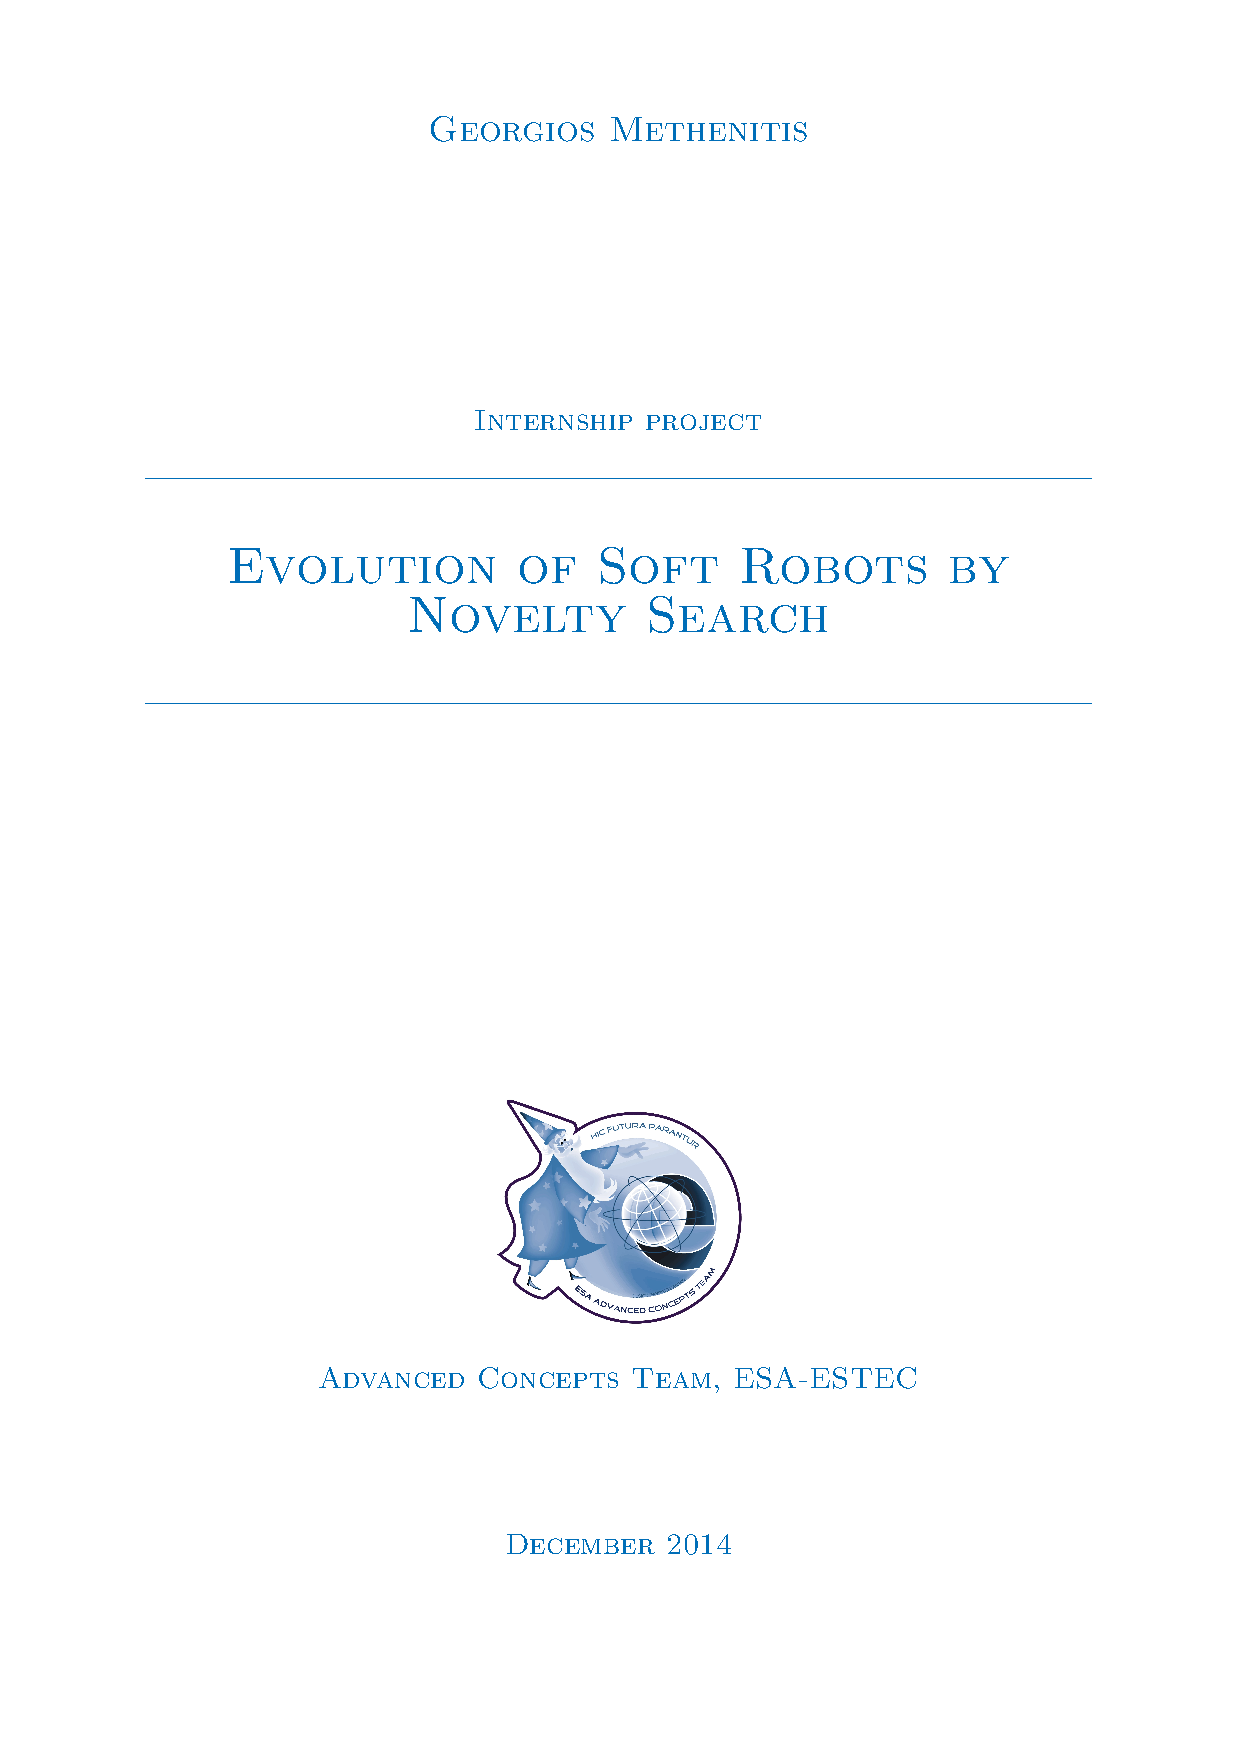
\includepdf[offset=2.55cm -2.55cm]{cover.pdf}
%----------------------------------------------------------------------------------------
%	TITLE PAGE
%----------------------------------------------------------------------------------------
\begin{titlepage}

\begin{center}

\includegraphics[width=.10\textwidth]{../Figures/Misc/University_of_Amsterdam_logo.pdf}\\[0.2cm]
\textsc{\Large \univname}\\[0.7cm] % University name
\textsc{\LARGE Master Artificial Intelligence}\\[2.0cm]
\vspace{0.1cm}% University/department logo - uncomment to place it
\textsc{\large Master Thesis}\\[0.5cm]
\HRule \\[0.4cm] % Horizontal line
{\huge \bfseries \ttitle}\\[0.4cm] % Thesis title
\HRule \\[1.5cm] % Horizontal line
\begin{minipage}[t][3.5cm][t]{0,4\textwidth}
\begin{flushleft} \large
\emph{Author:}\\
\authornames
\end{flushleft}
\end{minipage}
\begin{minipage}[t][3.5cm][t]{0,4\textwidth}
\begin{flushright} \large
\emph{Supervisors:} \\
\supname
\end{flushright}
\end{minipage}
\begin{flushbottom}
\begin{center}
ECTS: $42$\\[0.5cm]
\textit{Submitted to the Board of Examiners in partial\\ fulfillment of the requirements for the degree of \\\textbf{MSc. Artificial Intelligence}\\ of the\\ \textsc{University of Amsterdam}.}\\[2.5cm]
\large \today
\end{center}
\end{flushbottom}
\end{center}
\end{titlepage}

\cleardoublepage



%----------------------------------------------------------------------------------------
%	DECLARATION PAGE
%	Your institution may give you a different text to place here
%----------------------------------------------------------------------------------------

\clearpage % Start a new page

%----------------------------------------------------------------------------------------
%	QUOTATION PAGE
%----------------------------------------------------------------------------------------

\pagestyle{empty} % No headers or footers for the following pages

\null\vfill % Add some space to move the quote down the page a bit

\textit{``Evolve solutions; when you find a good one, don't stop."}

\begin{flushright}
David Eagleman, \textit{Incognito: The Secret Lives of the Brain}
\end{flushright}

\vfill\vfill\vfill\vfill\vfill\vfill\null % Add some space at the bottom to position the quote just right

\cleardoublepage % Start a new page

%----------------------------------------------------------------------------------------
%	ABSTRACT PAGE
%----------------------------------------------------------------------------------------

\addtotoc{Abstract} % Add the "Abstract" page entry to the Contents

\abstract{\addtocontents{toc}{\vspace{1em}} % Add a gap in the Contents, for aesthetics
Soft robotics is a vivid research field on the science and engineering aspects of soft materials in mobile machines. Recent development in soft robotics and evolutionary optimization have shown the possibility to simultaneously evolve the morphology and locomotion of soft robots. Generative encoding coupled with neural evolution of augmented topologies shows promising results. Novelty search, unlike traditional optimization methods does not aim to optimize the objective but instead looks for novelty. Novelty search rewards diversity and leads to a boundless variety of solutions, mimicking natural evolution. Apart from the performance comparison between novelty and fitness based search, this thesis shows that new locomotion patterns can be produced by the former. Different types of selection algorithms for fitness and novelty based evolution are studied, as well as, a method to combine both is proposed. Last but not least, the performance objective-wise is tested under variant gravity conditions leading into a taxonomy of possible locomotion strategies given different gravity levels.
}

\clearpage % Start a new page

%----------------------------------------------------------------------------------------
%	ACKNOWLEDGEMENTS
%----------------------------------------------------------------------------------------

\setstretch{1.3} % Reset the line-spacing to 1.3 for body text (if it has changed)

\acknowledgements{\addtocontents{toc}{\vspace{1em}} % Add a gap in the Contents, for aesthetics
The present work has been conducted in association with the \emph{Advanced Concepts Team} (ACT) in \emph{European Space Agency} (ESA-ESTEC, Noordwijk). The subject of this thesis had been offered as an internship project by ACT under the title: ``\textit{Simultaneous evolution of morphology and locomotion of soft robots by novelty search}''. Most of this work has been conducted during my $3$-month internship at ACT, ESA-ESTEC.

It would have been impossible to write this thesis without the help and support of my three supervisors, Arnoud Visser (Senior Lecturer, UvA), Dario Izzo (Scientific Coordinator, ACT) and Daniel Hennes (Postdoctoral Research Fellow, ACT).

I would like to thank Arnoud for his valuable comments in the whole duration of this thesis. I am grateful for all the discussion we had the last two years regarding my thesis, Dutch Nao Team, and the number of projects and papers we have done together.

I am most grateful to Dario and Daniel. Their ideas and discussions we had were valuable for me to finish this work. It has been an honor working under their supervision, as I gained too much from them.

I express my warm thanks to all the members of Dutch Nao Team, the Robocup SPL team of University of Amsterdam, in which I was proud to serve as a member for two years. I also thank all the members of ACT who welcomed me in the team and made my three-month internship a wonderful experience. Special thanks to Paul for our ``evolutionary'' conversations.

I would like to express my gratitude towards everyone who supported me during my master studies. Especially, my family, my friends, and my girlfriend. You have given me your unequivocal support throughout this work and my studies.
}
\clearpage % Start a new page

%----------------------------------------------------------------------------------------
%	LIST OF CONTENTS/FIGURES/TABLES PAGES
%----------------------------------------------------------------------------------------

\pagestyle{fancy} % The page style headers have been "empty" all this time, now use the "fancy" headers as defined before to bring them back

\newpage
\lhead{\emph{Contents}} % Set the left side page header to "Contents"
\tableofcontents % Write out the Table of Contents

\newpage
\lhead{\emph{List of Figures}} % Set the left side page header to "List of Figures"
\listoffigures % Write out the List of Figures

\newpage
\lhead{\emph{List of Tables}} % Set the left side page header to "List of Tables"
\listoftables % Write out the List of Tables

\newpage
\lhead{\emph{List of Algorithms}} % Set the left side page header to "List of Tables"
{\let\clearpage\relax\listofalgorithms}
\addcontentsline{toc}{chapter}{List of algorithms}

\clearpage % Start a new page

%----------------------------------------------------------------------------------------
%	ABBREVIATIONS
%----------------------------------------------------------------------------------------

%\clearpage % Start a new page
%
%\setstretch{1.5} % Set the line spacing to 1.5, this makes the following tables easier to read
%
%\lhead{\emph{Abbreviations}} % Set the left side page header to "Abbreviations"
%\listofsymbols{ll} % Include a list of Abbreviations (a table of two columns)
%{
%\textbf{LAH} & \textbf{L}ist \textbf{A}bbreviations \textbf{H}ere \\
%%\textbf{Acronym} & \textbf{W}hat (it) \textbf{S}tands \textbf{F}or \\
%}

%----------------------------------------------------------------------------------------
%	PHYSICAL CONSTANTS/OTHER DEFINITIONS
%----------------------------------------------------------------------------------------

%\clearpage % Start a new page
%
%\lhead{\emph{Physical Constants}} % Set the left side page header to "Physical Constants"
%
%\listofconstants{lrcl} % Include a list of Physical Constants (a four column table)
%{
%Speed of Light & $c$ & $=$ & $2.997\ 924\ 58\times10^{8}\ \mbox{ms}^{-\mbox{s}}$ (exact)\\
%% Constant Name & Symbol & = & Constant Value (with units) \\
%}

%----------------------------------------------------------------------------------------
%	SYMBOLS
%----------------------------------------------------------------------------------------

%\clearpage % Start a new page
%
%\lhead{\emph{Symbols}} % Set the left side page header to "Symbols"
%
%\listofnomenclature{lll} % Include a list of Symbols (a three column table)
%{
%$a$ & distance & m \\
%$P$ & power & W (Js$^{-1}$) \\
%% Symbol & Name & Unit \\
%
%& & \\ % Gap to separate the Roman symbols from the Greek
%
%$\omega$ & angular frequency & rads$^{-1}$ \\
%% Symbol & Name & Unit \\
%}

%----------------------------------------------------------------------------------------
%	DEDICATION
%----------------------------------------------------------------------------------------
\clearpage

\setstretch{1.3} % Return the line spacing back to 1.3

\pagestyle{empty} % Page style needs to be empty for this page

\dedicatory{This work is dedicated to my family. Thank you for your support during all the years I have been a student.} % Dedication text

\addtocontents{toc}{\vspace{2em}} % Add a gap in the Contents, for aesthetics

%----------------------------------------------------------------------------------------
%	THESIS CONTENT - CHAPTERS
%----------------------------------------------------------------------------------------

\mainmatter % Begin numeric (1,2,3...) page numbering

\pagestyle{fancy} % Return the page headers back to the "fancy" style

% Include the chapters of the thesis as separate files from the Chapters folder
% Uncomment the lines as you write the chapters

% Chapter 1

\chapter{Introduction} % Main chapter title

\label{Chapter1} % For referencing the chapter elsewhere, use \ref{Chapter1} 

\lhead{Chapter 1. \emph{Introduction}} % This is for the header on each page - perhaps a shortened title


Soft robotics is a field of research inspired by soft-bodied organisms, whereas the engineering and designing aspects of soft-structures are in the middle of interest, as soft-robotics can make the interaction between robots and living organisms safe, as well as their function in natural or more complex environments, where rigid robots have disadvantages. Actuated soft materials that react to environmental changes, add complexity to the designing phase of soft-robot engineering, since the degrees of freedom for soft structures that the distribution of materials and the space of possible morphologies, make the number of possibilities vast. 

Approaching such vast search spaces, is a heavy task, recent development in evolutionary optimization though, have shown the possibility of successful evolution of both the morphology and the locomotion strategy of soft robots, while the genotype representation is of vital importance to the evolution. Generative encoding for the genotype representation has shown promising results. Compared to direct encoding, where its representation is a direct mapping from genotype to phenotype level, generative encoding genotype is a function that is similar to a set of rules that can be queried for each coordinate in the Cartesian phenotype space and produce the output. Recent work has proved that evolutionary methods coupled with a generative encoding genotype representation can actually evolve both the morphology and the locomotion behavior of soft-robotics in a virtual simulation.

Traditional evolutionary methods in pursuance of the objective function defined by the user, are blind to keep enough diversity within the population, resulting usually driving the evolution towards local optima. Novelty search, unlike traditional optimization methods does not aim to optimize individuals towards an objective, but instead looks for novelty. Novelty search rewards diversity and leads to a boundless variety of solutions, mimicking natural evolution in such a way. Doing so, it has proven to be a successful method for searching vast spaces where the objective function is deceptive.

Passive soft-robotic structures have no limitations to the extent of morphologies, in the same context, gravity conditions when robot locomotion is investigated might be more decisive when it comes to the morphology of the robot explorers. With the freedom soft-structures can give to evolutionary techniques in respect to the designing part of the evolution (evolved morphology), it is of interest to validate that a taxonomy of different locomotion strategies can apply when the gravity conditions change.



\section{Thesis Contribution}

This thesis explores possibles ways of evolving the morphology and the locomotion strategy of soft structures under a virtual simulation environment. A simple genetic algorithm is used to confirm that these kind of problems cannot be captured by a simple genetic method, with direct encoding representation. Direct and direct encoding are also used under a random robot generator which show the advantages of the encoding in the produced structures, as well as point out the need of an indirect encoding to explore and exploit the geometrical properties of the problem. This encoding scheme is used paired to an evolutionary algorithm to verify results of previous work on the same domain, showing that generative representations for the genotype can indeed benefit these kind of evolutionary optimization methods. In addition, this thesis is exploring the effect of diversity based evolution can have in the performance of the evolved morphologies. Novelty search, a method rewarding the ``new'' in the behavior level is used for this purpose showing that not only same or better performance can be achieved through this method but also the diversity of behaviors is remarkably increased. \todo{write for different gravities...}






\section{Thesis Outline}

Chapter~\ref{Background}, provides some background information on the field of soft robotics, an introduction to genetic algorithms, different encoding techniques for the genomes, neuroevolution algorithms, and finally, objective driven search is presented and compared to novelty search. In Chapter~\ref{Related Work}, related material about evolutionary techniques for evolution of soft-robots morphology and locomotion is presented, in aspects of artificial life. Chapter~\ref{Method}, is a comprehensive documentation presenting details of the implementation of different evolutionary techniques. Chapter~\ref{Results}, gives a detailed presentation of the results achieved under variant techniques. Next, in chapter~\ref{Future Work}, future applications and extensions of this work provided. Chapter~\ref{Conclusion}, serves as an epilogue to this thesis, where some important points of it are presented.
% Chapter 2

\chapter{Background} % Main chapter title

\label{Background} % For referencing the chapter elsewhere, use \ref{Chapter1} 

\lhead{Chapter 2. \emph{Background}} % This is for the header on each page - perhaps a shortened title

This chapter gives an overview of the state-of-the-art methods in evolutionary algorithms. It gives an in-depth discussion about the intersection of evolutionary algorithms and robotics. This discussion focuses mostly on how evolutionary methods are used to evolve robot designs and controllers for some applications. In addition, genetic algorithms, the role of the encoding in the representation within an evolutionary setting,  how artificial neural networks (ANNs) can represent an organism in evolutionary algorithms (EAs), and how these ANNs can be evolved when coupled with an EA are presented. As part of the different encoding schemes, an indirect coding called compositional pattern-producing networks is also discussed in detail. Additionally, the aspect of the objective function in such evolutionary problems and the effect it has on the performance of the methods is studied. Furthermore, novelty search, a method which uses an objective function that rewards diversity in the evolution is presented in detail. Last but not least, the field of soft robotics  is introduced, in conjunction with ways where these soft material structures can be evolved and simulated in virtual simulation environments. Soft robots, designed for real life applications are also presented.




\section{Evolutionary Algorithms}

Evolutionary algorithms (EA) are a part of the evolutionary computation field where generic population-based optimization algorithms are studied. Initially, an evolutionary process holds a fixed number of solutions which are randomly generated. These candidate solutions are propagated within generations until a good solution is found or a maximum number of iterations has passed. One of the most important advantages of EAs is that they can approximate good solutions in very complex optimization problems, where analytic methods cannot be applied. The non-deterministic nature of evolutionary algorithms starting with candidate solutions randomly sampled from the solution space does not guarantee that the evolution will always come up with the same results on independent runs. Another important fact of EAs is that holding a population of solutions can help avoid being ``trapped'' in local optima of a specific function. The way EAs propagate from one generation to the other is simply by using all or part of the current candidate solutions to produce the next generation. In evolutionary algorithms, the objective function is the measure that all solutions are evaluated against in order to reach the ultimate goal of the optimization problem.




\subsection{Genetic Algorithms}
\label{geneticAlgorithms}
Genetic algorithms are part of the evolutionary algorithms following the same principles.

\begin{quote}``Genetic algorithms are probabilistic search procedures designed to work on
large problem spaces involving states that can be represented by strings.''\end{quote}

Considering the above quote~\citep{goldberg1988genetic} a genetic algorithm is a process of evolving a string-stream of values, which is a single solution in a high dimensional problem space. These values can be at their simplest form bits ($0, 1$), integers, floats or char values.

Each of these candidate solutions is called a \emph{phenotype} and the stream from which the solution is derived, \emph{genotype} or \emph{chromosome}. Each generation holds a population of a fixed number of individuals which are initially randomly selected out of a distribution over the solution space. The iterative process that follows and creates a new population of individuals, given the current population, is called \emph{generation}. Usually the algorithm terminates after a fixed number of generations or when the goal has been reached. 

The way the next generation's population is produced depends on the current population; Genotypes are selected to breed new individuals. There are two basic ways for a new genotype to be produced. The first way is called \emph{mutation} and requires only one individual from the current population. Mutation will change one or more values in the \emph{chromosome} of the selected individual to create a new one and maintain the genetic diversity from one generation to the other. \emph{Crossover} is the second basic genetic operator and requires two or more parents for each new individual. This operator is similar to biological crossover and it uses parts from all parents to create a new chromosome. 


The way individuals are selected after each successful generation in order to produce new individuals belongs to the genetic process of \emph{selection}. Selection as the name reveals itself selects which individuals will become parents and which individuals will not. The selection criteria as it also happens in some natural environments where the fittest organisms survive is a function that can approximate the goodness of a given solution. This \emph{objective} function, also called \emph{fitness}, is a measure of how good an individual is, i.e. total displacement of a robot's body while trying to evolve walking. With the knowledge of the fitness function added to the evolution, weak individuals are most of the times discarded from the breeding process. Selecting parents randomly from the top part of the population or selecting parents via \emph{tournament}, are two of the basic selection methods in evolutionary algorithms. The former ensures that only a small part (i.e top $20\%$ ({\it survival threshold})) of the current population will survive. In the contrary, tournament selection also known as \emph{Competition}, allows the whole population to breed, while it randomly picks a fixed number of individuals selecting the best among those. A third way of choosing individuals for the next generation is called \emph{Elitism}. Elitism is a genetic selection technique. When used, it is responsible for copying a mutation or an actual copy of the best individual of the current generation to the next. It ensures that during the evolution successful solutions will carry on living and share their ``valuable'' genes into the next generations.

\begin{figure}[t!]
\vspace{0.4cm} % leave more space
\centering
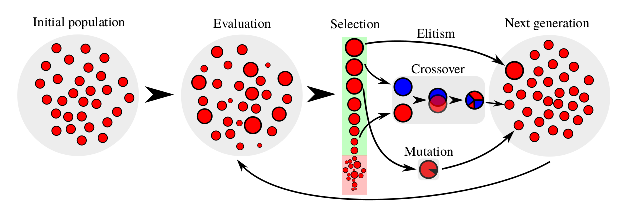
\includegraphics[width=0.8\textwidth]{../Figures/Misc/Evolution.eps}
\caption{Basic pipeline of an evolutionary method.}
\label{fig:evolutionPipeline}
\end{figure}


Figure~\ref{fig:evolutionPipeline} illustrates the general algorithmic pipeline of an evolutionary method, as described above. This starts with a random initialized population which is then evaluated (size refers to how ``good'' each individual is). All individuals are then sorted based on their goodness in respect the objective function. The selection process follows, where a set of the best individuals is selected to produce the next generation. Elitism, alongside crossover and mutation are used to this proportion of the population. The next generation will also be evaluated in respect to the same objective function and the iterative process will continue.

\section{Evolutionary Robotics}
\label{sec:evolutionary_robotics}

Evolutionary robotics~\citep{nolfi2001evolutionary} (ER) is a method that makes use of evolutionary computation algorithms to evolve the control and/or the morphology, without the direct design by engineers. Most research concentrates on developing robot controllers for simulated or real robots~\citep{harvey1997evolutionary,nolfi1994evolve}. One big advantage of this method is that it can evolve solutions for environments that designers and engineers do not have enough knowledge about (i.e., designing a robot controller for another planet, where surface type and gravity level might be crucial variables for the design of an exploring robot). In the same fashion as natural evolution, evolutionary techniques work with a population of random initialized controllers or designs. The candidate population individuals (robot controllers) used in ER applications may be drawn from some subset of the set of artificial neural networks (ANNs), whereas simpler versions of genetic algorithm applications use bit-streams that directly map the controller. The controllers in the best performing robots are then selected, altered and propagated through mutation, crossover, and other genetic operations, in a repeating process that mimics natural evolution. Evolutionary robotics is done with many different objectives, often at the same time. These include creating useful controllers for real-world robot tasks, reproducing biological phenomena, etc.. Creating controllers via artificial evolution requires a large number of evaluations of a large population. This usually takes a lot of computational time, which is one of the reasons why evolution of such controllers is usually evaluated within a simulation software. Initial random controllers may exhibit potentially harmful behavior, such as repeatedly crashing the robot into a wall, which may damage a physical robot.

Apart from evolutionary methods to develop robot controllers reinforcement learning~\citep{hayes1994robot,mahadevan1992automatic} can be used rewarding actions, resulting to state-action pairs that lead to high rewarding behaviors. As a result, a robot controller can be indirectly built. Applying evolved robot controllers to real robots in a physical environment is an extremely difficult task, since simulators in front of the limitations of computing efficiency sacrifice the accuracy~\citep{jakobi1995noise}. As mentioned earlier, evolutionary methods can be used to design the physical structure (morphology) of a robot~\citep{hiller2010evolving}, in addition to or in place of the controller. This thesis is exploring this aspect of evolution, the simultaneous evolution of the morphology and the locomotion of virtual soft robots. 

Developmental robotics~\citep{lungarella2003developmental,asada2001cognitive,weng2004developmental,asada2009cognitive} is a field related to evolutionary robotics,  while instead of evolving through generations towards fitter controllers, it is trying to mimic life-like learning starting from a ``blank'' state in which the robot's ``brain'' is initialized and every variable of the environment is unknown.

\begin{figure}[t!]
\centering
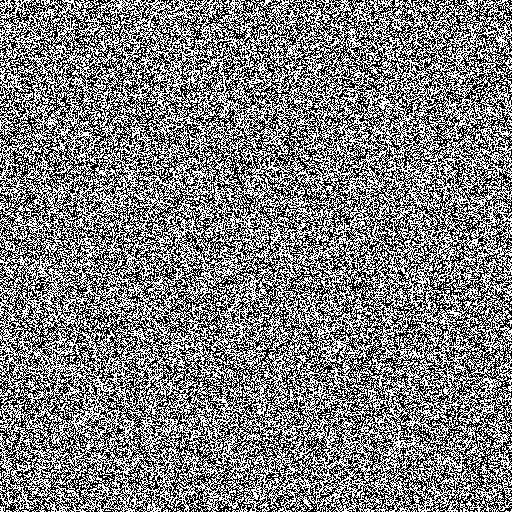
\includegraphics[width=0.3\textwidth]{../Figures/Misc/direct.jpg}\  \   \   

\includegraphics[width=0.3\textwidth]{../Figures/Misc/indirect.jpg}
\caption{Comparison of direct encoding versus generative for the binary image example.}
\label{fig:directVsIndirectEncoding}
\end{figure}


\section{Direct-Indirect Encoding of the Genotype}
\label{DirectIndirect}

A simple direct encoding was described in the previous section, when a single dimension stream of bits or numbers described the chromosome. When the dimensions of the task define the length of the genome, we refer to \emph{direct} encoding, which means that the genotype-phenotype mapping is a straightforward function. An example of this encoding could be the design of a two dimensional binary image. In direct encoding the genotype of this picture can be represented by a stream of bits which has the same length as the number of pixels of the image. In other cases, where there is no direct mapping between the genotype and the phenotype, indirect encoding is present, where a set of rules or a function maps the genotype to the phenotype space. In cases the phenotype space can be represented by a Cartesian n-dimensional space, an indirect encoded chromosome can be a function that is queried for each coordinate in a specific resolution and represents the phenotype. For the same binary image example, indirect encoding would be a function that gives pixel values $0$ or $1$ for every pixel's coordinate. 



Figure~\ref{fig:directVsIndirectEncoding} illustrates the difference between direct and indirect encoding. An example binary image is shown for both encoding schemes, in the first case (direct encoding) the genotype is a binary stream which length is equal to the number of pixels producing the value of each pixel directly. The latter encoding uses a genome of length 3, as many as the coefficients of the linear combination in the following function: 
\[f(x,y) = c_1 sin(x) + c_2 cos(x) + c_3 tan(y)
\]
the result is taken after applying the same function for each pixel coordinate. Even in cases where a simple function is used, the  phenotype holds some of its functions properties such as symmetry and repetition, resulting in a pattern that direct encoding cannot produce.

A method that can represent more complex functions and is widely used to indirectly map the genotype to the phenotype space is the \emph{artificial neural networks}. Artificial neural networks (ANNs) are computational models which are inspired by living-organisms central neural system (Brain). These models are used to approximate functions that are generally unknown, using a set of nodes and connections between pairs of nodes. Each connection within the network holds a weight which used as a multiplicative factor of each signal passing through the connection. Nodes are then responsible of propagating the summation of the signal received from the connections by a Sigmoid function. This interconnected set of nodes can propagate the inputs fed into the network to one or more output nodes, approximating in this way a complex non-linear function.


\begin{figure}[t!]
\centering

\includegraphics[width=0.25\textwidth]{../Figures/Misc/cppnNetwork.eps}
\caption{Compositional pattern-producing networks have identical network structure with artificial neural networks while they make use of a canonical set of activation functions.}
\label{fig:cppnNetwork}
\end{figure}



\subsection{Compositional Pattern-Producing Networks}
\label{CPPN}

Encoding plays an important role and it is critical to the performance of evolutionary algorithms especially when large problem spaces are present. Research has shown that the genotype-phenotype mapping can affect performance~\citep{komosinski2001comparison} in three dimensional agents, where more complex encoding schemes outperform direct encoding. In addition, geometrical implications of the problem also have some potentially important roles in the encoding. The role of symmetry to the encoding is crucial especially in applications like board games, robot controllers, biped walking, etc.. In these cases, geometric regularities of the encoding can be essential to the performance of the evolutionary method.

\begin{figure}[t!]
\centering
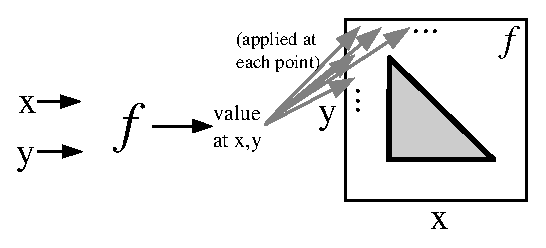
\includegraphics{../Figures/Misc/cppnResolution.eps}
\caption{CPPNs work as a function $f$ that is being queried for the whole n-dimensional Cartesian space in which space the phenotype is mapped, in this case the phenotype is the triangle in a two-dimensional space, figure taken by~\citep{stanley2007compositional}.}
\label{fig:cppnResolution}
\end{figure}

\emph{Compositional pattern-producing networks}~\citep{stanley2007compositional} or CPPNs are artificial neural networks with an extended set of activation functions (see Fig.~\ref{fig:cppnNetwork}). Results by this encoding show that regular patterns can be produced in this generative mapping from the genotype to the phenotype space. Like in the previous two dimensional image representation of a phenotype, CPPNs generate phenotypes that can be interpreted as distributions of points in a multidimensional Cartesian space. The genotype (CPPN) can then be queried for each coordinate of the space and gives the phenotype representation of the genotype in multiple resolutions. In the same fashion, images can be constructed using CPPNs, where pixel coordinates are queried to the network and the grayscale or RGB values can be taken by the outputs of these networks. 


Figure~\ref{fig:cppnResolution} illustrates how the mapping between the genotype and phenotype is done using generative encoding (CPPNs). A major asset of CPPNs is that they can generalize in all resolutions. Considering the previous figure (see Fig.~\ref{fig:cppnResolution}), the CPPN is queried for all $x,y$ coordinates of the phenotype two dimensional Cartesian space. The step of $x,y$ sampling can be determined by the problem, since the inputs of the CPPN are the normalized coordinates $x,y \in [-1,1]$. Hence, genotypes using this kind of generative encoding can be mapped in every resolution, making this process straighforward to generalize. As the space of the phenotype becomes larger, a generative encoded solution (CPPN) is not affected by the increasing dimensions of the problem, a constraint that heavily affects direct encoding.

\begin{figure}[t!]
\centering
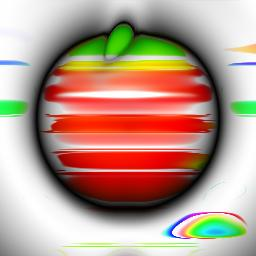
\includegraphics[width=0.25\textwidth]{../Figures/Misc/picBreed3.jpg}\quad   
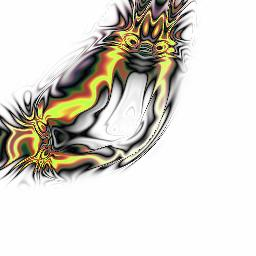
\includegraphics[width=0.25\textwidth]{../Figures/Misc/picBreed2.jpg}\quad
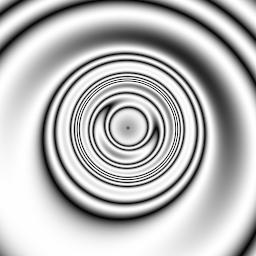
\includegraphics[width=0.25\textwidth]{../Figures/Misc/picBreed1.jpg}\\
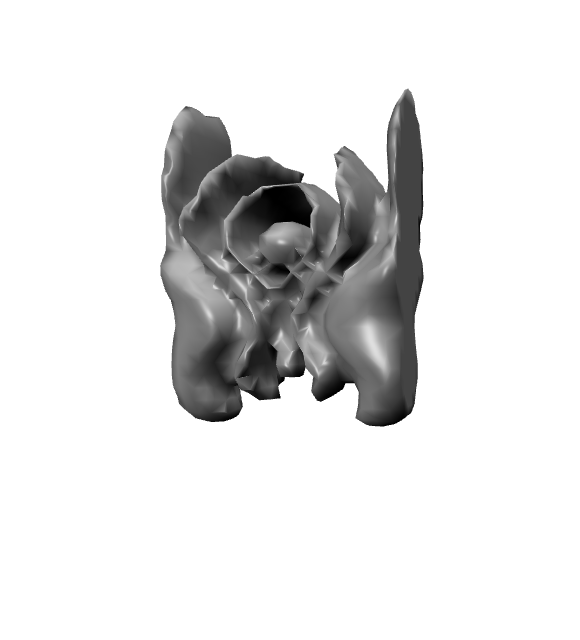
\includegraphics[width=0.25\textwidth]{../Figures/Misc/endless2.png}\quad 
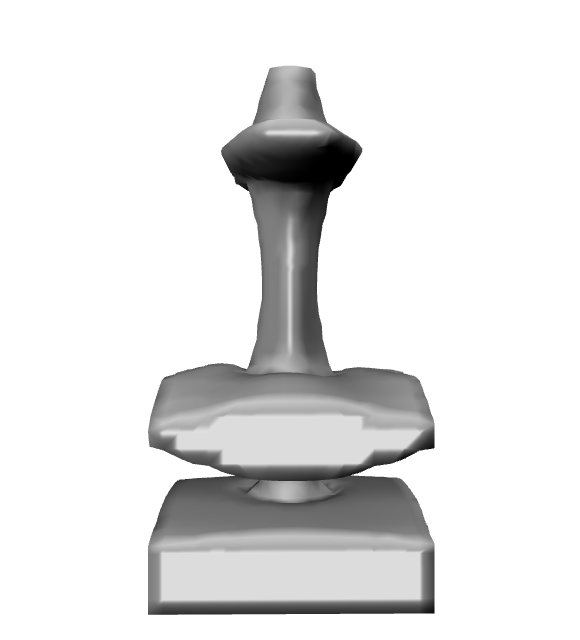
\includegraphics[width=0.25\textwidth]{../Figures/Misc/endless1.png}\quad
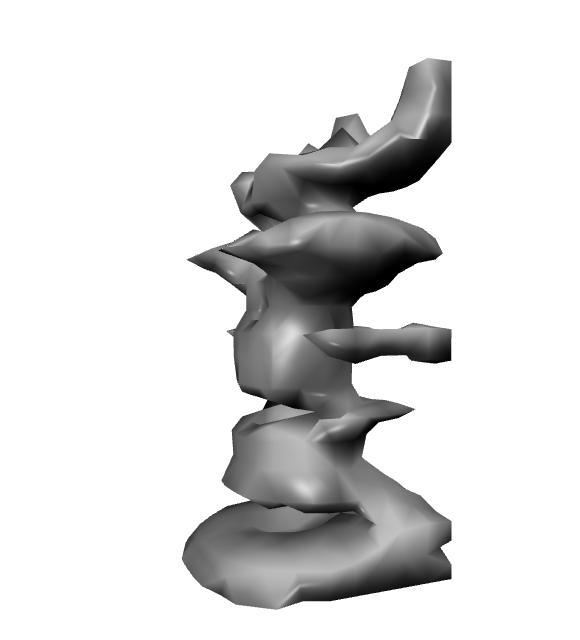
\includegraphics[width=0.25\textwidth]{../Figures/Misc/endless3.png}
\caption{Compositional pattern-producing networks can encode truly complex images\protect\footnotemark[1] (top) and 3D-structures\protect\footnotemark[2] (bottom).}
\label{fig:cppnImages}
\end{figure}

\footnotetext[1]{picbreederSite: \url{http://www.picbreeder.org}}
\footnotetext[2]{EndlessForms: \url{http://www.endlessforms.com}}

Compositional pattern-producing networks have been used in many applications where symmetry and repetition can produce two or three dimensional artistic structures\footnotemark[2], and drawings\footnotemark[1]~\citep{secretan2008picbreeder}. As these applications require more symmetrical properties than others, not only Cartesian space coordinates are fed into the inputs of these networks, but more inputs biasing the network should be present~\citep{secretan2008picbreeder}. Some example inputs that can be fed into the network as additional inputs are the distance from the center of the space or the distance from the center to one axis. Figure~\ref{fig:cppnImages} illustrates images encoded by CPPNs. Comparing the results with Figure~\ref{fig:directVsIndirectEncoding}, it is understandable why this kind of encoding can capture solutions in problem domains where symmetry is important.




\section{Neuroevolution}

\emph{Neuroevolution}~\citep{yao1997new} is an optimization technique using evolutionary methods as described in Section~\ref{sec:evolutionary_robotics}, where artificial neural networks take the place of simpler encoding methods. ANNs can compute arbitrarily complex functions, learn and perform under the presence of noisy inputs and generalize to unseen sensory information. Neuroevolution requires only a measure of a network's performance at a task, which can be used as the reward for good solutions (ANNs) to survive. More complicated forms of chromosome representations can develop more complex robot controllers. After each run, the sensory input of the task domain is given at the artificial neural network's input neurons and the solution is given by the output of the networks where the fitness of the specific brain can be evaluated. A major issue is the selection of the network's \emph{topology}. Topology is the arrangement of the network's elements such as links and nodes, which represents the structure and how the information flows within the network. In early neuroevolution methods the topology of the networks used was fixed, meaning that the only elements of the networks evolving were the weights of the connections between the nodes. In modern neuroevolution methods, the topology of the networks is also subject to the evolution.

\begin{figure}[t!]
\centering
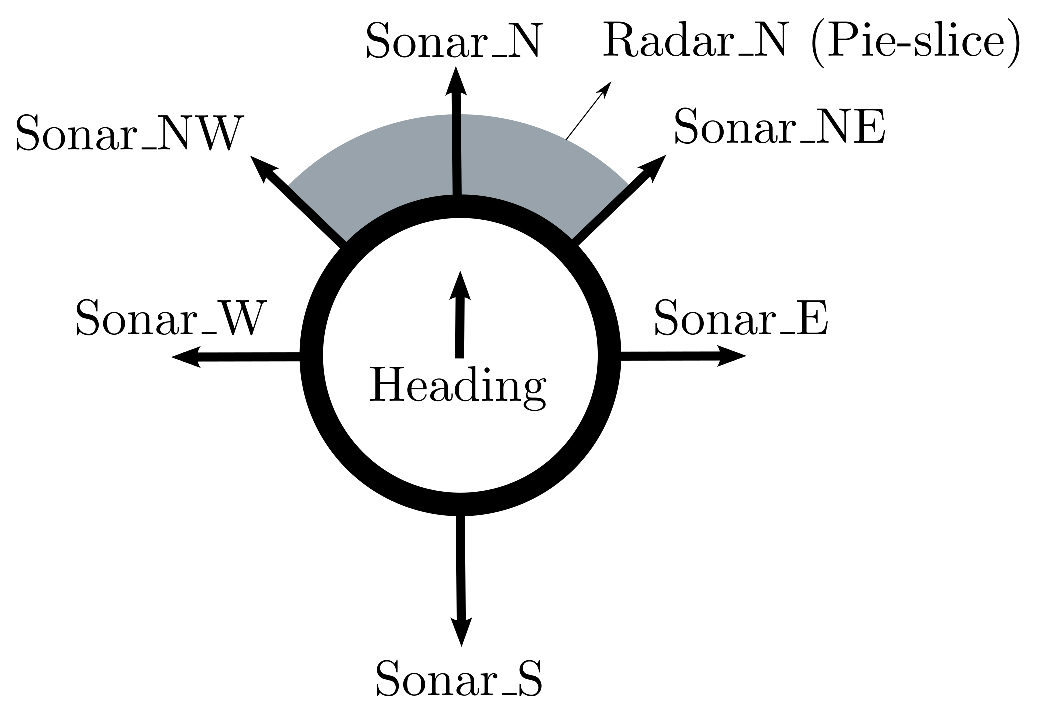
\includegraphics[width=0.35\textwidth]{../Figures/Misc/RobotMaze.eps}\  \    \  \    
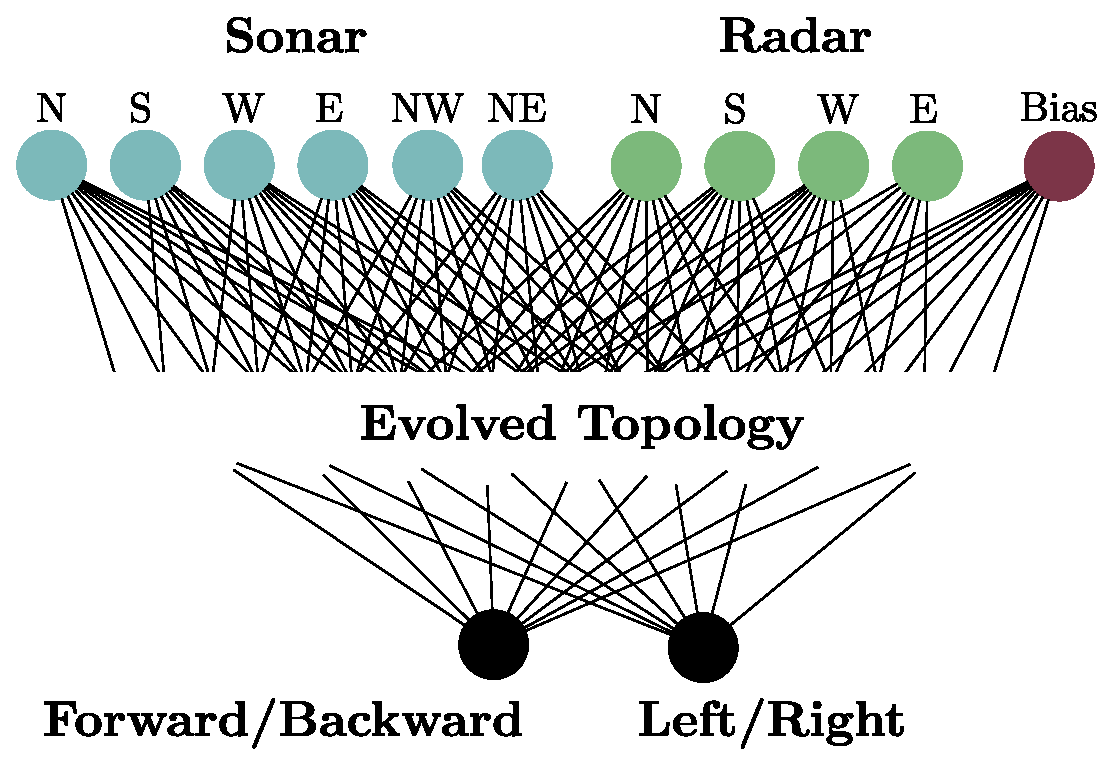
\includegraphics[width=0.49\textwidth]{../Figures/Misc/RobotMazeNetwork.eps}
\caption{Robot controllers can be evolved through neuroevolution algorithms where robot sensors are the inputs of neural networks while the outputs directly control the robot.}
\label{fig:robotExample}
\end{figure}


\subsection{Neuroevolution of Augmented Topologies}
\label{NEAT}

Neuroevolution of augmented topologies (NEAT) as it was first introduced by~\citep{stanley2002evolving} is also a neuroevolution method used to evolve artificial neural networks. A major advantage of this method is that alongside the weights it also evolves the topologies of the networks within the population.

Originally, neuroevolution methods were developed to capture difficult sequential decision making, as well as to control problems. The sensory information is the input of these neural networks and decisions are the outputs. NEAT is yet another method for evolving ANNs where a few extra features are added, enables finding solutions in more demanding problems. NEAT starts the evolution process with a population of networks with simple topologies. Through the generations instead of just fixing the weights of the networks' connections, topologies are becoming more complex allowing nodes and links to be added. Meaning that during the evolution, more complicated networks will be produced, this \emph{complexifying} technique leads to capturing more demanding solutions as it offers enough freedom to the evolution.

Figure~\ref{fig:robotExample} illustrates how sensory information can be given as input to a neural network. The neural network, given the sensory information provided, controls the robot which tries to drive itself close to a target position in a maze. The outputs of the network completely control the motion of the robot. All the sensory information (six sonar sensors which output the distance from the closest obstacle in six directions and 4 pie-slice radar sensors which are only activated when the target position is located within the range of each one covers) is available to the controller.

Several aspects of this method worth mentioning where \emph{speciation} is one of the most important. Speciation is the procedure that protects new \emph{species} until they have enough time to evolve before comparing them with the rest of the population. For two individual genotypes (ANNs) to belong to the same species their network topology must be similar, meaning that a threshold is set and a function determines the numeric value of two network topologies' similarity. Two different genotypes (ANNs) can share shame genes (topologies within the network) and their compatibility (genotype similarity) is given by:
\begin{equation}
\label{CompatibilityEquation}
\delta = c_1 \cfrac{E}{N} + c_2 \cfrac{D}{N} + c_3 \bar{W}
\end{equation}
where $E$ is the number of \emph{Excess} genes (genes that do not match and they do not occur in parents' genotype), $D$ is the number of \emph{Disjoint} genes (genes that do not match but they occur in parents' genotype), $\bar{W}$ is the average weight difference between \emph{Matching} genes (Identical) and $N$ is the number of genes in the larger genotype used for normalization.
The age of each species protects them for competing in equal terms with more optimized species, giving them in this way time to evolve further towards the objective function.



\section{CPPN-NEAT}

Compositional pattern-producing networks as described earlier in this chapter (see Sec. \ref{CPPN}) are similar computational methods to ANNs in regards to their structure, so one can make use of the \emph{complexifying} property to capture in this way more complex solutions (behaviors). NEAT method can evolve CPPNs in the place of ANNs, since it only needs few modifications. 

The resulted method that evolves this generative type of genomes (CPPNs) is called CPPN-NEAT~\citep{stanley2007compositional} and its only difference in respect to the original NEAT algorithm is the way new nodes are added to the network. The original NEAT algorithm evolves ANNs which are using sigmoid functions at every node, so every new node will carry this function.
In the contrary, CPPNs use a variety of functions from a canonical set. CPPN-NEAT assigns a random function from this set to every newly added node. 

Experiments~\citep{stanley2007compositional} have shown that this method can indeed evolve CPPNs capturing in this way solutions in problems with geometrical properties (i.e board games, biped walking, etc.). NEAT is holding the properties of natural evolution as every neuroevolution method. Furthermore, NEAT coupled CPPN encoding can be used to determine the connectivity (topology) of artificial neural networks in  a method called HyperNEAT~\citep{stanley2009hypercube}.




\section{Novelty Search}
\label{NoveltySearch}

Traditional search within the framework of evolutionary algorithms needs an objective function, a function that guides the search towards ``good'' areas of the solution space following the gradient of the fitness. Defining the fitness function is a straightforward problem most of the time. In a problem where a robot tries to get to a target from its initial position in a room with no obstacles in between a fitness function could be defined as the Euclidean distance between the final position of the robot and the target point, the closer it gets to the target the more points (higher fitness) the specific controller is rewarded.

\subsubsection*{When the objective function misleads the search}

\begin{figure}[t!]
\centering
\begin{subfigure}[b]{0.3\textwidth}
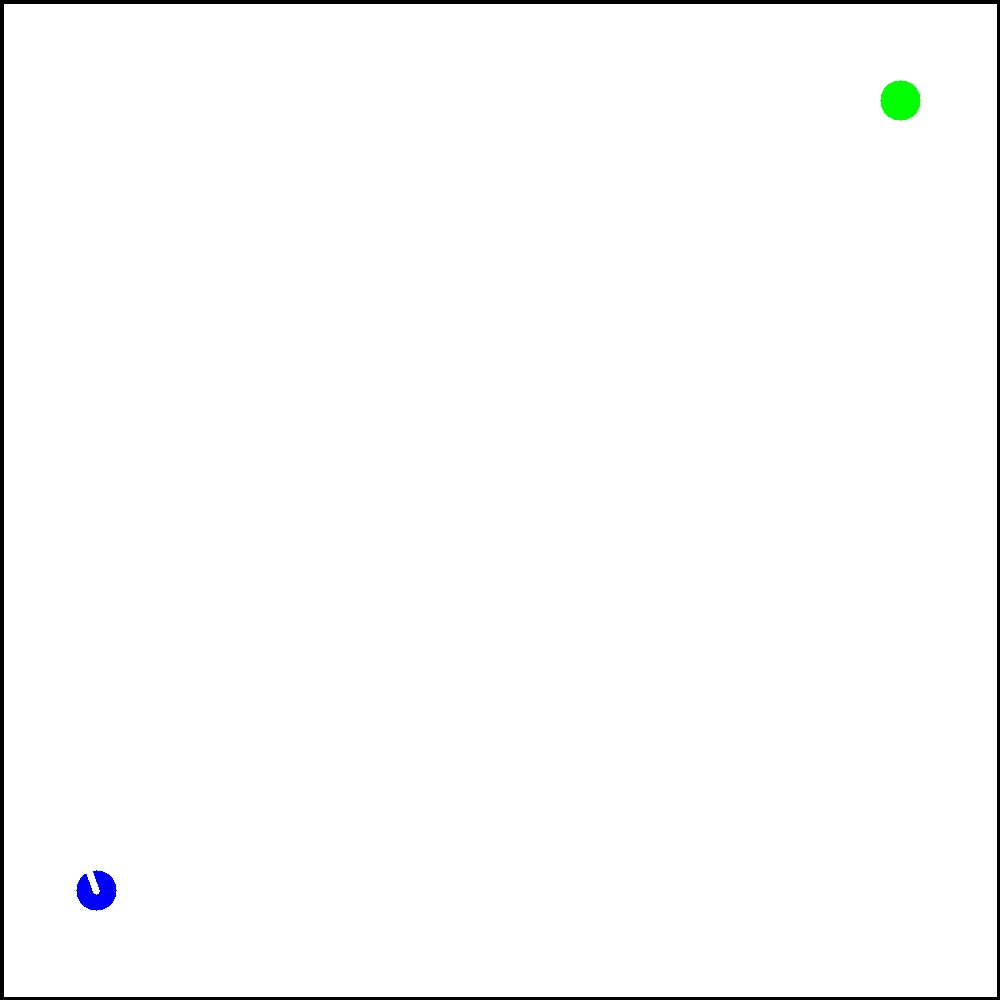
\includegraphics[width=1.0\textwidth]{../Figures/Misc/MazeEasy.jpg}
\caption{Easy}
\label{fig:mazeEasy}
\end{subfigure}\hspace{2cm} 
\begin{subfigure}[b]{0.3\textwidth} 
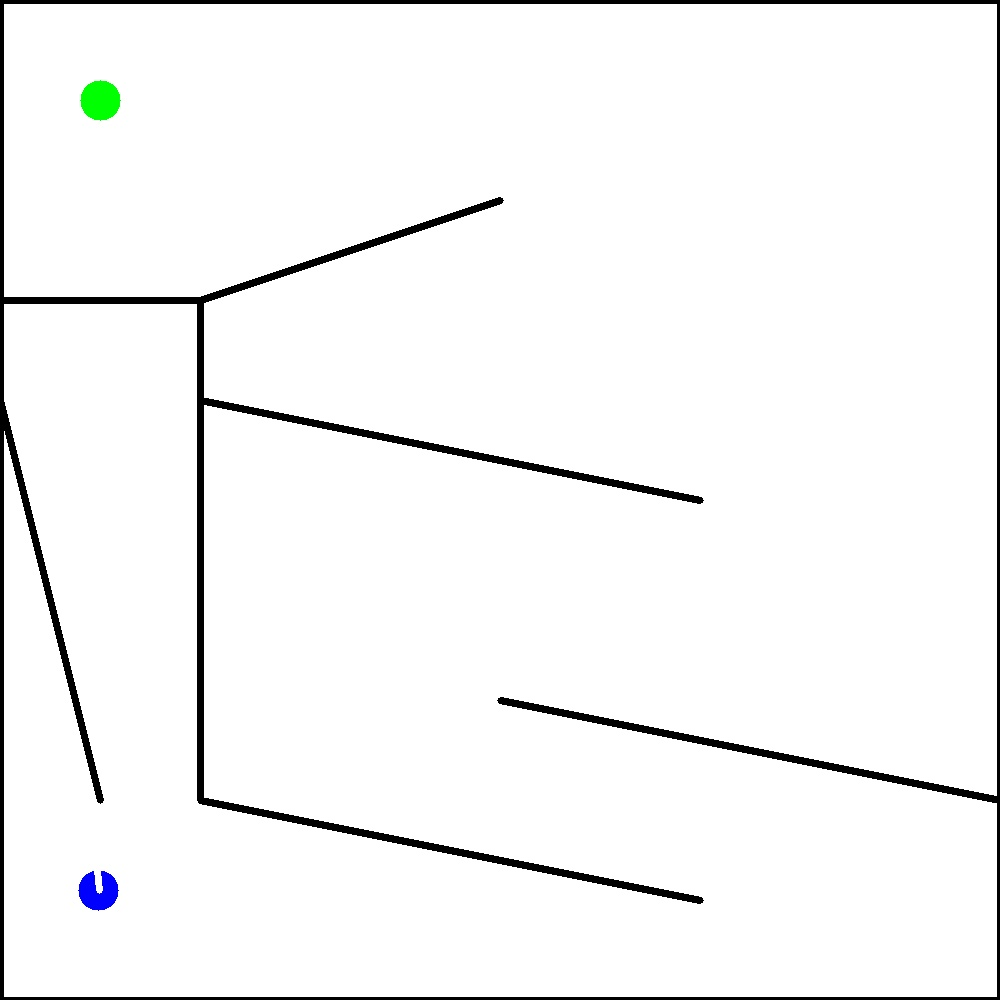
\includegraphics[width=1.0\textwidth]{../Figures/Misc/MazeHard.jpg}
\caption{Hard}
\label{fig:mazeHard}
\end{subfigure}
\caption{An objective function can be devious. Maze examples from~\citep{lehman2011abandoning}.}
\label{fig:maze}
\end{figure}

An objective function as the one described above is greedy, driving the search directly towards highly rewarding areas of the solution space. In cases that local optima can be found in the landscape of the objective function this greedy fitness measure can drive and trap the evolution in these localities of the problem.

Considering the robot-maze example presented in~\citep{lehman2011abandoning,lehman2010revising}, a robot (\textcolor{Blue}{blue} dot) is placed in a maze (see Fig.~\ref{fig:maze}), the robot (see Fig.~\ref{fig:robotExample}) has multiple sensory information which are fed as inputs to its controller (``brain''). The controller is driving the robot through the maze having only sonar and radar sensory information, while its ultimate goal is to drive the robot to the target position (\textcolor{Green}{green} dot) in a fixed time span. Naturally, to select a fitness function that can give enough information about how good a controller is the Euclidean distance  from the final position of the robot to the target position is measured in the end of the simulation time. For the first maze (see Fig.~\ref{fig:mazeEasy}) when no obstacles are between the robot and its target the objective function is reliable, since the Euclidean distance to the target indeed informs the robot how close it is located. In the second maze (see Fig.~\ref{fig:mazeHard}) using the same fitness function search can be mislead. In this example maze achieving high fitness does not mean that the robot is actually close to the target. Driving north in this maze following the increasing fitness leads to a wall that cannot be passed by the robot. Therefore, exploration is needed in low fitness areas which will allow the robot to reach the target point with the maximum fitness. The deceptive nature of the fitness function in this problem can be found in a lot of optimization problems, while the walls in this maze clearly denote problems where this fitness landscape can be found. 

\begin{figure}[t!]
\centering
\begin{subfigure}[b]{0.3\textwidth}
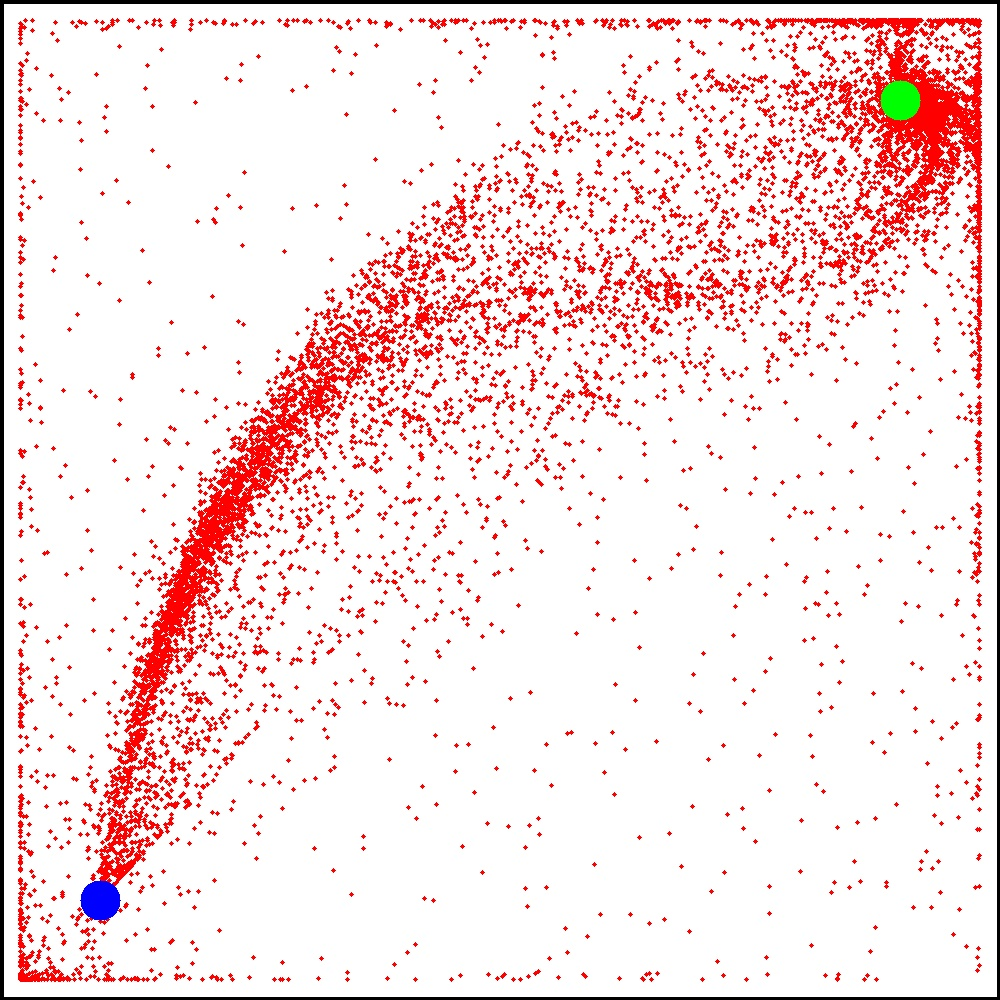
\includegraphics[width=1.0\textwidth]{../Figures/Misc/MazeEasyFitness.jpg}
\caption{Visited space after $200$ generations.}
\label{fig:mazeFitnessEasy}
\end{subfigure}\hspace{2cm}
\begin{subfigure}[b]{0.3\textwidth}
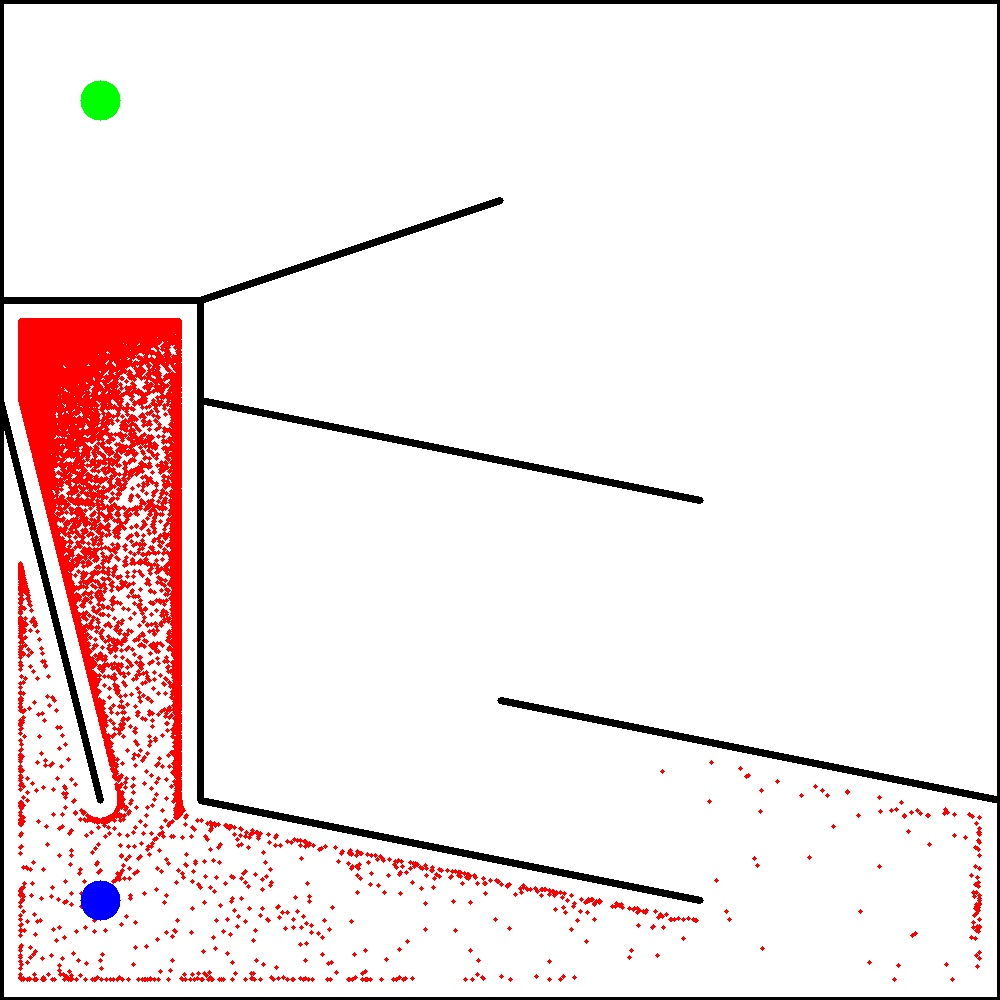
\includegraphics[width=1.0\textwidth]{../Figures/Misc/MazeHardFitness.jpg}
\caption{Visited space after $1000$ generations.}
\label{fig:mazeFitnessHard}
\end{subfigure}
\caption{Fitness search has no problems to find the solution in the easy map, while it can not find the optimal solution in the hard setting after $250.000$ evaluations.}
\label{fig:mazeFitness}
\end{figure}


To visualize how fitness based search can fail in such a setting Figure~\ref{fig:mazeFitness} presents the results of the above experiment explained using the robot sensory information presented in Figure~\ref{fig:robotExample}. NEAT algorithm is used to evolve the neural controller presented in the same figure. The settings used for this experiment were the same as in~\citep{lehman2011abandoning} where a population of $250$ individual controllers per generation was used. As it was expected, fitness based search was successful in the easy setting (see Fig.~\ref{fig:mazeFitnessEasy}). However, it failed to find the optimal solution in the hard map (see Fig.~\ref{fig:mazeFitnessHard}) focusing on creating controllers that lead the robots drive north until the wall was reached, failing to explore the map extensively.

\subsubsection*{Natural evolution is not an evolution towards fitness}

Using an objective function in evolutionary computation and typically reward individuals which are closer to an objective is far away from natural selection in the evolution process, where exploration is allowed as long as the criteria for survival hold~\citep{lehman2010revising}. Driving search towards promising parts of the fitness space where local optima may be present ensures that other areas of the search will not be explored, leading search to stay and explore the nearby area while more promising regions are far away in the solution space. Solutions located in these regions are called \emph{stepping stones}~\citep{lehman2008exploiting,lehman2011abandoning,lehman2010revising,risi2009novelty}. Stepping stones are points in the solution space that may not be good as far as their objective values are concerned, but can eventually lead to better or the global optima of a specific optimization problem.


\subsubsection*{Search for novelty}

Novelty search~\citep{lehman2008exploiting,lehman2011abandoning,lehman2010revising, risi2009novelty} unlike traditional fitness based search is an alternative way of optimization towards an objective function without having knowledge of this objective. In simple words it is looking for a solution to a problem without knowing how close it is to solve it; fact that turns out to have a major impact to the increased performance of this method in several problem domains. 

What novelty search seeks for is how interesting a new solution is in respect to all previously found ones. To define ``interesting'' we need to move our point of interest into behavior space which is a function of each phenotype, similar to the fitness function. Nevertheless, it fully or partially describes the behavior without directly implying the fitness function. As an example someone can think of a behavior could be defined as the final position of the navigation robot or the trajectory of it in the previous robot-maze example. Rewarding behaviors of the phenotype that are different from the previously found ones drives the evolution to visit new points in the behavior search space.

One significant point here is that the behavior space in some domains can be limitless. However, a valid behavioral metric can be found excluding behaviors that are meaningless or do not comply with the natural limits of the problem. On the other hand, the search space in the genotype level can also be infinite especially in neuroevolution methods like NEAT where ANNs can grow during the evolution. A bounded space of understandable-valid behaviors is then the key idea of novelty search where increasingly complex behaviors present to the evolution as the complexity of the genotype grows along.

Multi-objective optimization can also make use of a novelty metric alongside fitness, trying to optimize both at the same time~\citep{mouret2011novelty}. Another method that exploits the diversity of the produced genomes in order to map the phenotype to the fitness is also proposed by the literature~\citep{mouret2012algorithm}.

\subsubsection*{Is novelty search similar to random?}

Initial thoughts are converging that novelty search is similarly behaving to random search, constantly looking for something new in the vast space of behaviors. It seems similar to evolving random robot controllers without considering the behavior aspect of their phenotypes hoping that enough exploration will be done in both genotype and phenotype spaces. A random approach having no information about the observed behaviors the evolved phenotypes produce is not able to drive the evolution since different and more complex genotypes can easily produce similar behaviors. The novelty in the behavior level assures that the search will explore deeply the behavior space with the hope that a \emph{fit} behavior will be found. Aside from that, novelty search does not perform backtracking which ensures that it will constantly drift away from already generated behaviors (i.e similar behaviors to already generated ones result to low novelty value). At the same time there is no such guarantee in random search. Therefore, it is certain and proven later in this thesis that no exploration in the behavior space will be performed by random search.



\subsubsection*{How can novelty be measured?}

As fitness is a function to measure the ``goodness'' of an individual, novelty measures how different an individual is from all previously found individuals. To define different a novelty metric measures the difference in the behavior space of the phenotype. Given the phenotype's behavior $x$ a novelty measurement could be a function of $x$, $f(x)$ which computes how different (novel) is the specific behavior in respect to a set of other behaviors $S$ in behavior space.  As defined in~\citep{lehman2008exploiting,lehman2011abandoning} \emph{sparseness} can give a good measurement of how sparse is the area of a newly observed behavior. Given the behavior we can compute the sparseness by:
\begin{equation}
\label{sparsenessEquation}
f(x) = \cfrac{1}{k} \sum_{i=1}^{k} dist(x, S_i)
\end{equation}
where $S$ is a sorted set of the closest behaviors. Sparsity measures the average distance from the $k$-closest behaviors.


\subsubsection*{Algorithm}

\begin{figure}[t!]
\centering
\begin{subfigure}[b]{0.3\textwidth}
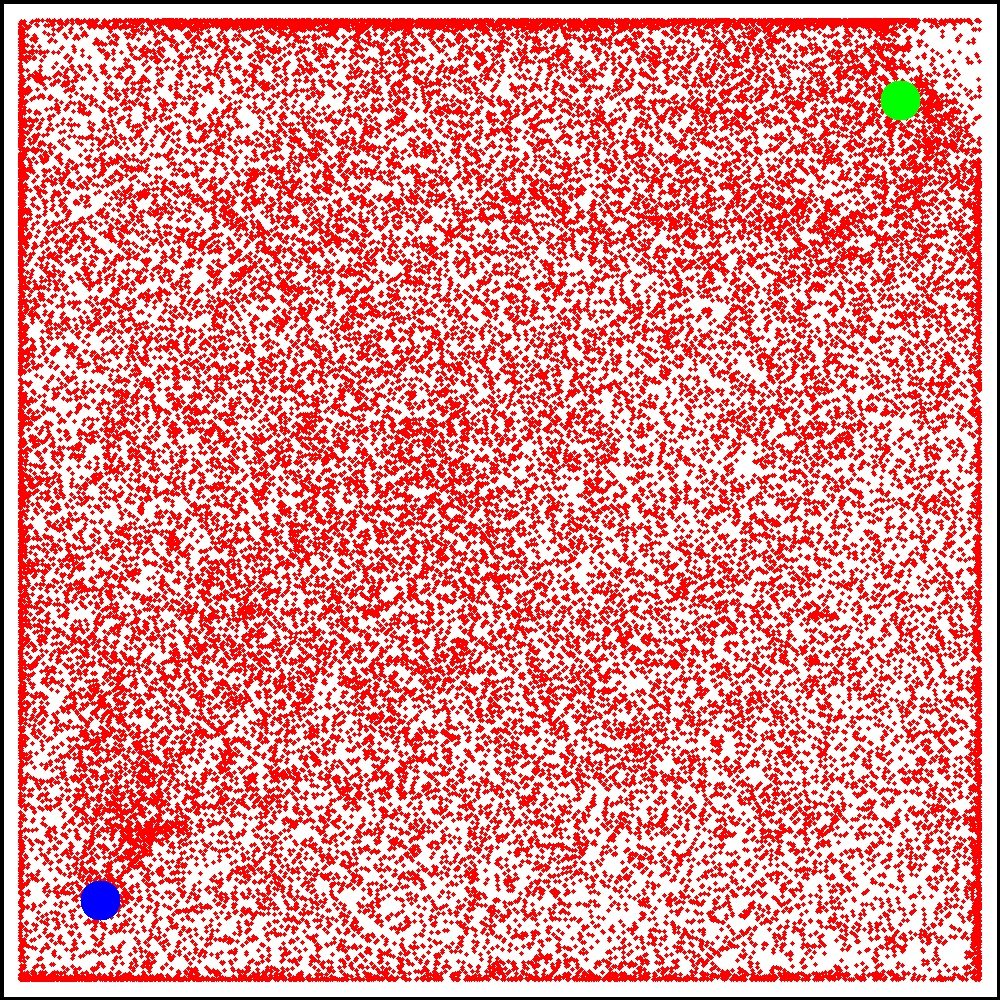
\includegraphics[width=1.0\textwidth]{../Figures/Misc/MazeEasyNovelty.jpg}
\caption{Visited positions in the map after $200$ generations.}
\label{fig:mazeNoveltyEasy}
\end{subfigure}\hspace{0.3cm}
\begin{subfigure}[b]{0.3\textwidth}
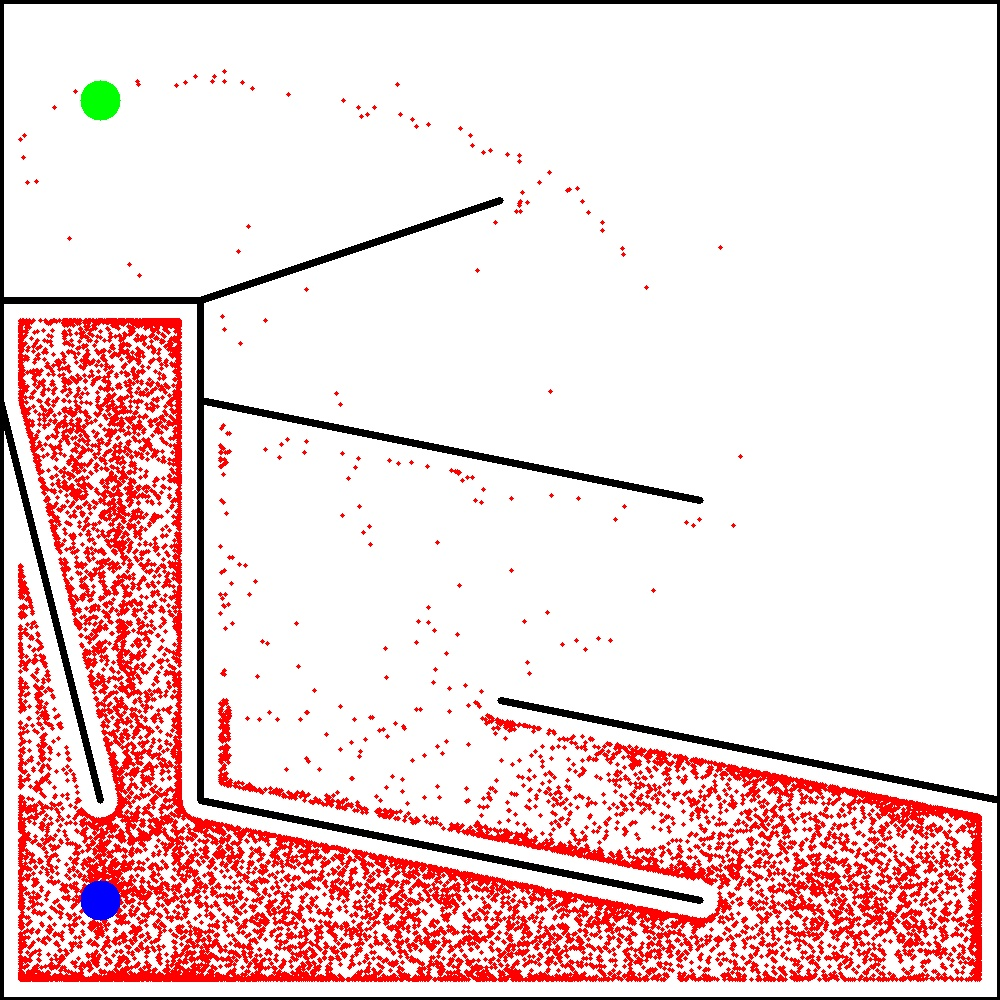
\includegraphics[width=1.0\textwidth]{../Figures/Misc/MazeHardNoveltySolution.jpg}
\caption{Solution found after only $80$ generations.}
\label{fig:mazeNoveltyHardSolution}
\end{subfigure}\hspace{0.3cm}
\begin{subfigure}[b]{0.3\textwidth}
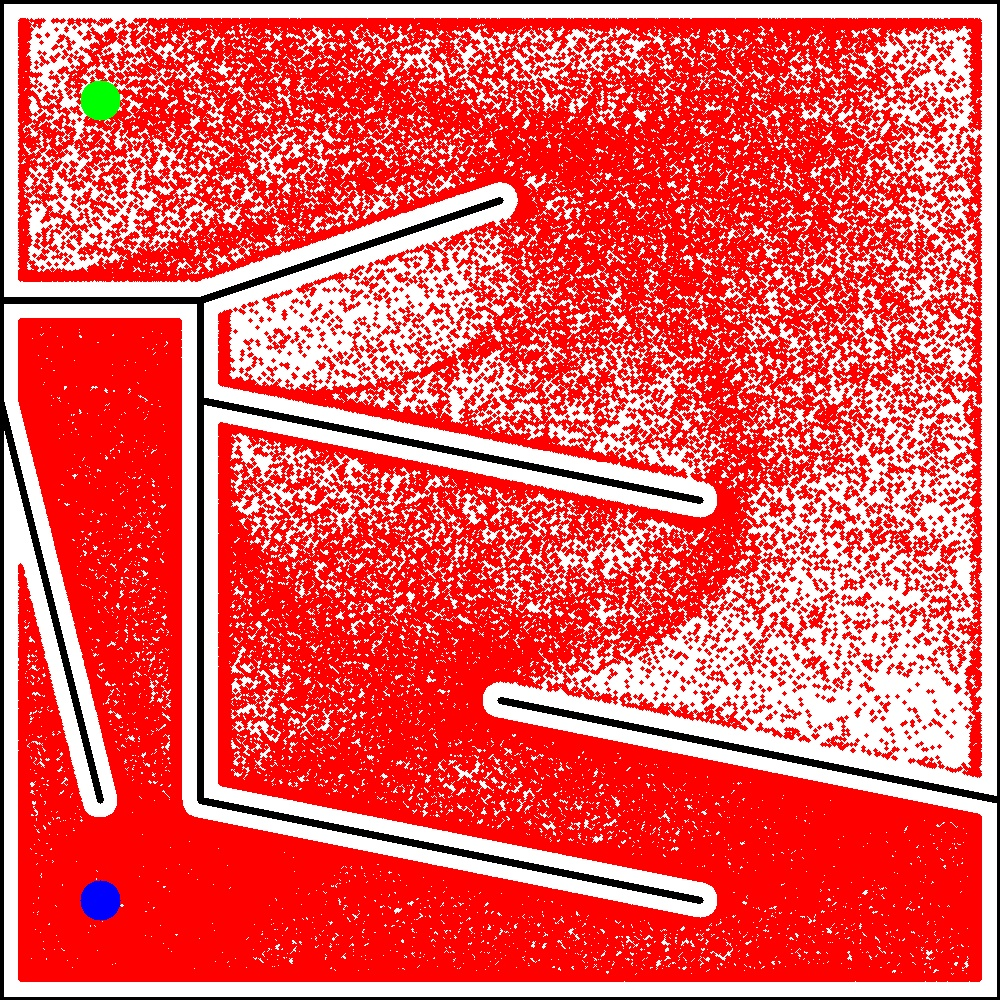
\includegraphics[width=1.0\textwidth]{../Figures/Misc/MazeHardNovelty.jpg}
\caption{ Visited positions in the map after $1000$ generations.}
\label{fig:mazeNoveltyHard}
\end{subfigure}
\caption{Novelty search applied in the robot-maze optimization problem. Novelty search deeply investigates the behavior space finding the solution even in the hard map setting.}
\label{fig:mazeNovelty}
\end{figure}


Replacing fitness with a novelty value is not the only modification any evolutionary algorithm needs in order novelty search to be implemented. To push search to visit new areas in the behavior space rewarding novel behaviors coming up during the evolution is needed. For this reason, storing novel reference points in space (behaviors) during the evolution is inevitable. The sparseness of a new behavior is computed by Equation~\ref{sparsenessEquation} resulting in a numerical value that implies how novel is the observed behavior of an individual phenotype. If the new behavior has a novelty value more than this threshold it is stored in the set of novel individuals. Apart from comparing any new behavior with all the novel behaviors, the newly produced one can also be confronted with the entire set of behaviors produced by the population in the same generation of the evolution. 

Having discussed the basic idea behind novelty search and how it can be implemented, it is time to apply it in a known problem where fitness based search failed. Considering the robot (see Fig.~\ref{fig:robotExample}) - maze (see Fig.~\ref{fig:maze}) example presented in this section, novelty search is now taking the place of evolution towards the objective function used before which was the distance to the goal. For the novelty metric to be evaluated, a behavior metric has to be defined, which in this case can be the final position of the robot by the time the simulation is finished. The sparsity measure then computes the reward of the robot based on how sparse the observed behavior of the robot in regards to all novel behaviors found before in the evolution is, based on the sparsity equation (see Eq.~\ref{sparsenessEquation}) using $k = 10$. Figure~\ref{fig:mazeNovelty} presents the results achieved by novelty search in this setting by showing all the visited areas that robots were driven to by their evolved controllers. In the easy setting map (see Fig.~\ref{fig:mazeNoveltyEasy}), novelty search achieved to fully explore every possible position in the map. In the hard map (see Fig.~\ref{fig:mazeNoveltyHardSolution}, \ref{fig:mazeNoveltyHard}), where fitness based search failed to find any solutions close to the target position, novelty search succeeded to do so after only $80$ generations.



\section{Soft Robotics}
Soft robotics is a highly promising field of research dedicated to the science and engineering of soft materials in mobile machines. As the name suggests soft robots~\citep{trivedi2008soft, pfeifer2012challenges} are made entirely of soft materials mimicking animals or animal-parts that consist only of soft tissue (elephant trunk, tongue, worm, octopus, etc.). Having no rigid parts in their design the degrees of freedom are infinite and the possible ways of motion can become extremely complex. In traditional robotics, joints and rigid parts predefine the space of possible movement and sometimes restrict the robot's locomotion strategy or \emph{gait} to a specific set. In soft robotics, the absence of rigid parts can on the one hand make the design of the locomotion strategy exceptionally tortuous, on the other hand the gait alternatives are limitless.

\begin{figure}[t!]
\centering
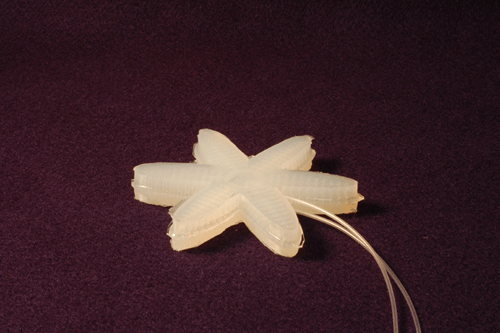
\includegraphics[width=0.3\textwidth,height=0.13\textheight]{../Figures/Misc/soft_robotics_figure.png}\		
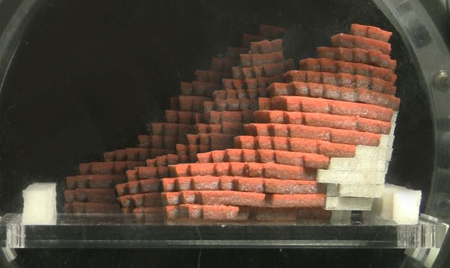
\includegraphics[width=0.3\textwidth,height=0.13\textheight]{../Figures/Misc/hillerPressureChamber.png}\	
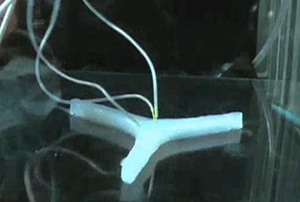
\includegraphics[width=0.3\textwidth,height=0.13\textheight]{../Figures/Misc/ExplodingRobot.jpg}\\
\caption{Soft robots can be actuated through air pressure tubes (left), pressure variations (middle), or internal explosions (right).}
\label{fig:softRobotsActuation}
\end{figure}

The design and development of soft robotics is not an easy task, while the actuation of such soft structures is the most challenging task. Actuating soft materials can be done in many ways including pneumatic systems~\citep{ilievski2011soft, shepherd2011multigait}, hydraulic, internal body explosions, passive actuation triggered by pressure or temperature variations and others~\citep{laschi2012soft, seok2010peristaltic}. Figure~\ref{fig:softRobotsActuation} illustrates three different ways that soft robot bodies can be actuated. Gripping mechanisms~\citep{hirose1978development} can softly and gently conform to objects of any shape and hold them with uniform pressure. This gripping function is realized by means of a mechanism consisting of links and series of pulleys which can be simply actuated by wires. Regardless traditional ways of actuating soft material robots, three dimensional printing is now giving the freedom for multi-material structures to be created, which also explodes the number of possibilities for the design of a soft structure such as a gripper soft robot. Topological optimization techniques can be applied~\citep{hiller2009multi} for producing functionalities in the design. Autonomously actuated soft robots~\citep{tolleyresilient} (see Fig.~\ref{fig:softbot}) can also be designed having multiple advantages over rigid body robots such as resistance under extreme temperatures and the capability of locomotion on terrains of variant types. 

Although soft robotics research field is in an early stage, it is growing fast. Some of the characteristics that make soft robots interesting to explore are the infinite number of degrees of freedom and the variety of materials (mostly elastic) that can be used, in the contrary to rigid robotics that are mostly made out of metals and plastic. Nevertheless, structure design and control of soft robotics remain challenging mostly because of their soft bodies can only be represented in continuous state spaces, where only analytic methods can be proven successful.

To sum up, locomotion capabilities of soft robots, as well as the possibilities of passive movement (i.e materials that actuate reacting to environmental changes) makes them an interesting topic for present and future research. Finally, considering also that soft materials are safer than conventional robot materials to humans, human-robot interaction can benefit from this field~\citep{sanan2011continuum}.


\begin{figure}[t!]
\centering
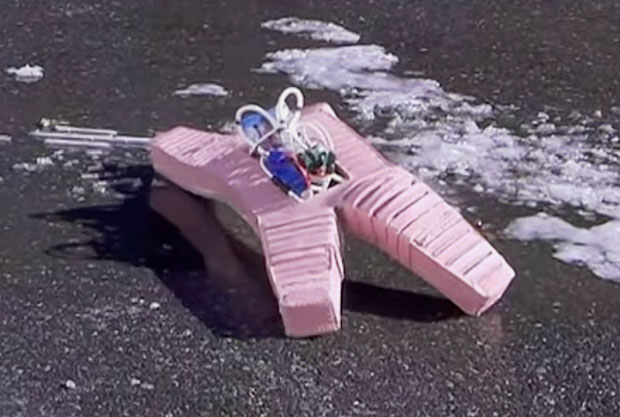
\includegraphics[width=0.6\textwidth]{../Figures/Misc/softbot.jpg}
\caption{Autonomously actuated soft robot~\citep{tolleyresilient}, it is able to withstand extreme temperatures and variant terrain types.}
\label{fig:softbot}
\end{figure}


\subsection{Soft Robotics in Simulation}

Most work to simulate interactions and deformations within and between soft material bodies are mostly focused on the graphical part of the problem~\citep{faloutsos1997dynamic} sacrificing the accuracy of the simulation~\citep{teschner2004versatile}. Three dimensional meshes~\citep{muller2002stable} can represent these bodies including the dynamics of their materials. 

A recent work though, \emph{VoxCad} simulator~\citep{hiller2012dynamic} is focusing mostly on the physics side of the soft material interactions not at the expense of a low frame rate. \emph{VoxCad} is a modeling and analyzing open-source software that can simulate soft material deformations and interactions. In Figure~\ref{fig:VoxCAD} the graphical user interphase of VoxCad software is presented during the simulation of the soft body robot in the simulator.

VoxCad cannot model and simulate three dimensional meshes, yet a lattice is used to represent the 3D workspace where voxels (three dimensional pixels) can be assigned different materials. Materials themselves are passive and cannot actuate without external trigger. In this simulator this external force that can actuate the materials is the temperature of the environment. The main variables of the environment is the base, the amplitude and the period of the temperature. Furthermore, gravity acceleration of the environment can vary. Materials have properties such as the elasticity of the material, density, Poisson's ratio, coefficient of thermal expansion (which determines how materials will be expanded in respect to the environment's temperature), temporal phase in respect to the temperature period, and the ground friction coefficients. Materials can also be mixed together to create a new type of material.

\begin{figure}[t!]
\centering
\includegraphics[width=1.0\textwidth]{../Figures/Misc/voxcad.png}
\caption{VoxCAD (Voxel CAD), a cross-platform open source voxel modeling and analyzing software.}
\label{fig:VoxCAD}
\end{figure}

Throughout this thesis, the terms \textit{structure} or \textit{soft robot} will refer to a set of connected voxels (not unconnected parts) within the lattice space. The voxel dimensions are constant through the experiments of this thesis, while the lattice space is variant. Since the voxel dimensions are the same for all settings, the term \textit{resolution} will be referring to the number of voxels in each dimension. Note that different resolutions also refer to different dimensions for the lattice as the voxel size is fixed.  For experimental settings used during the simulations see appendices~\ref{SimulationSettings}, \ref{ExperimentalSettings}. 




\begin{comment}
\section*{\todo{Additional Material that can be added later}}
\citep{stanley2003taxonomy}
\citep{nelson2009fitness}
\citep{meyer1998evolutionary}
How the Body Shapes the Way We Think A New View of Intelligence~\citep{pfeifer2007body}
\citep{albu2008soft}
\citep{woolley2011deleterious}
\citep{lewis1992genetic}
\citep{lapeyre2011maturational}
\citep{oudeyer2013intrinsically}
\citep{gauci:gecco07}
\end{comment}

% Chapter 3

\chapter{Results} % Main chapter title

\label{Results} % For referencing the chapter elsewhere, use \ref{Chapter1} 

\lhead{Chapter 3. \emph{Results}} % This is for the header on each page - perhaps a shortened title

\section{Results}

\clearpage
\subsection{Fitness Based Search}

\begin{figure}[h!]
\centering
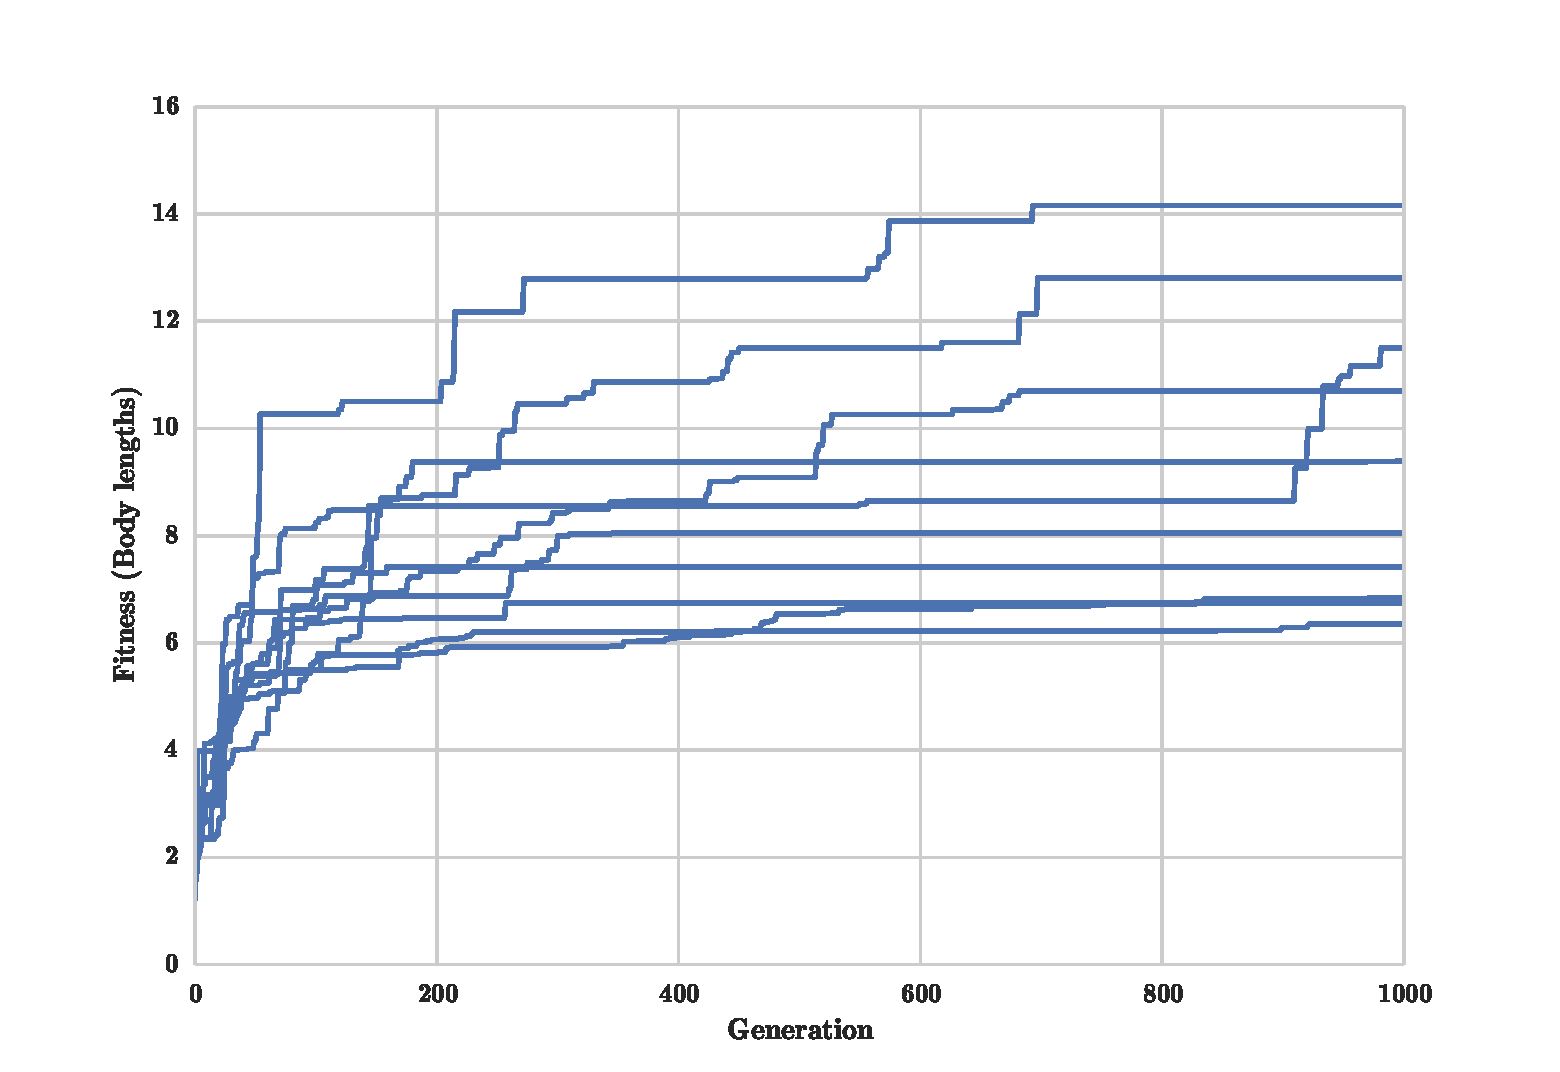
\includegraphics[width=1.0\textwidth]{Figures/Results/indRunsSize10Fitness.pdf}
\caption{Caption}
\caption{Best so far fitness in body lengths displacement of softbot's center of mass from $10$ runs for fitness based search. The gravity acceleration for this experiment used was $-27.468\   m/s^2$, the size of the lattice $10\times 10\times10$ and $4$ available materials ($2$-actuated).}
\end{figure}

\begin{figure}[h!]
\centering
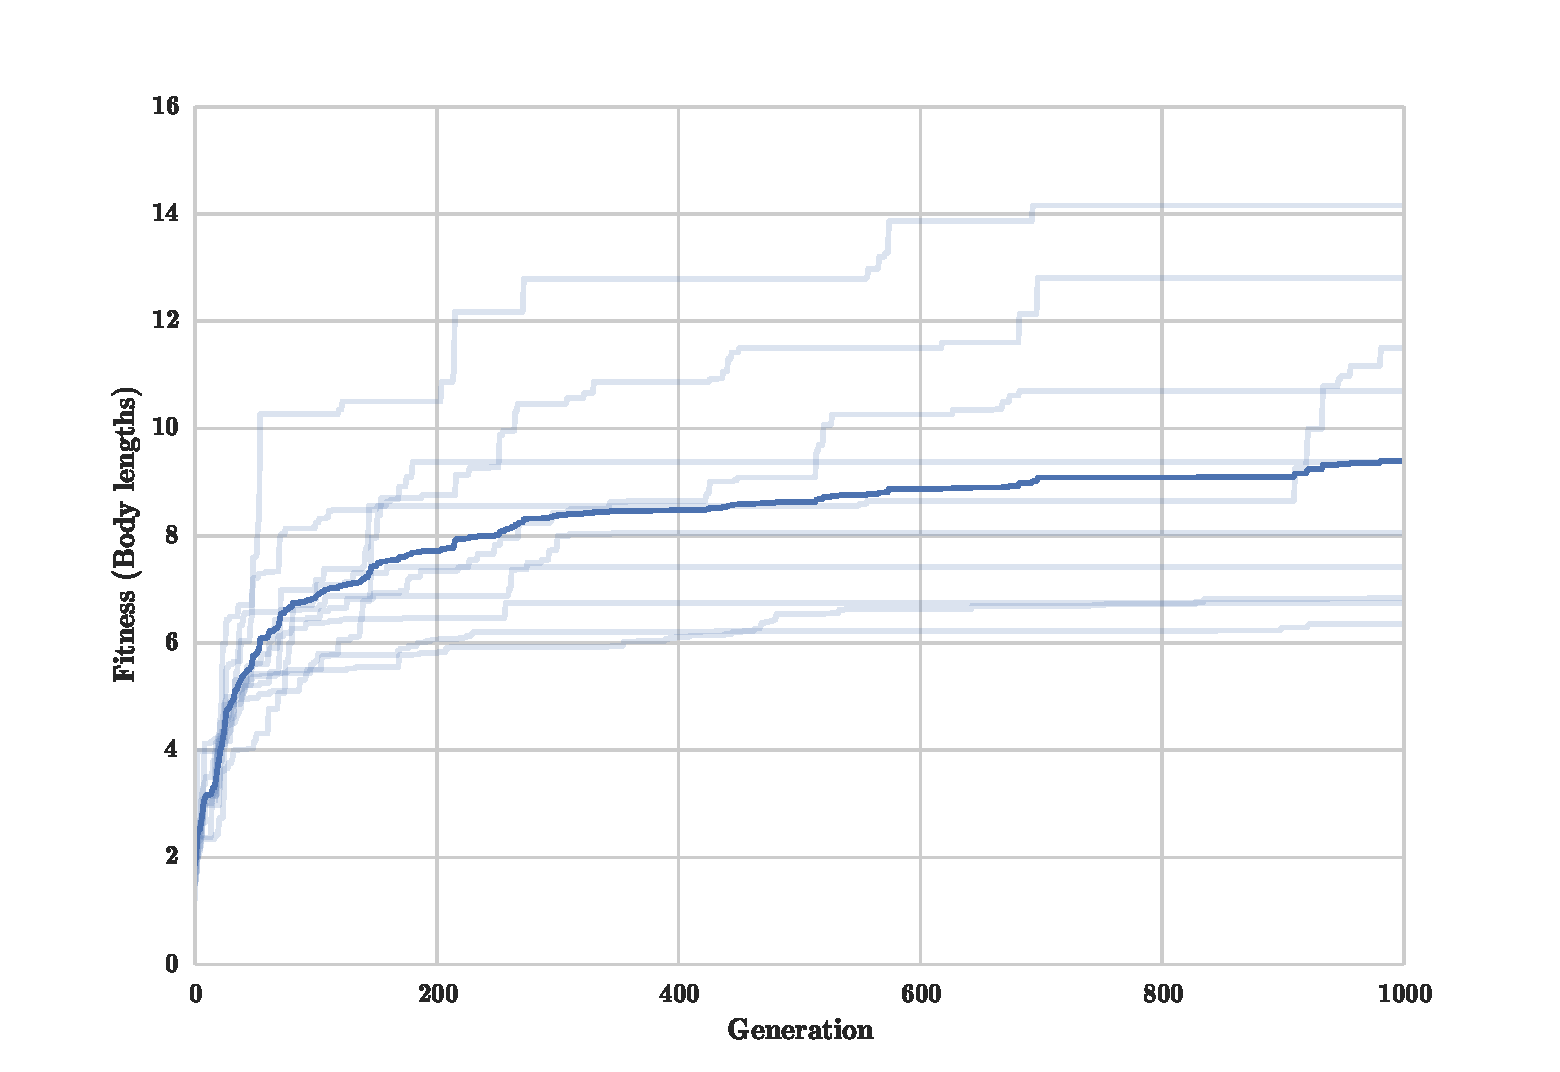
\includegraphics[width=1.0\textwidth]{Figures/Results/indRunsAvgSize10Fitness.pdf}
\caption{Best so far fitness in body lengths displacement of softbot's center of mass from $10$ runs together with their mean (thick line) for fitness based search. The gravity acceleration for this experiment used was $-27.468\   m/s^2$, the size of the lattice $10\times 10\times10$ and $4$ available materials ($2$-actuated).}
\label{fig:indRunsAvgSize10Fitness}
\end{figure}















\clearpage
\subsection{Novelty Search}

\begin{figure}[h!]
\centering
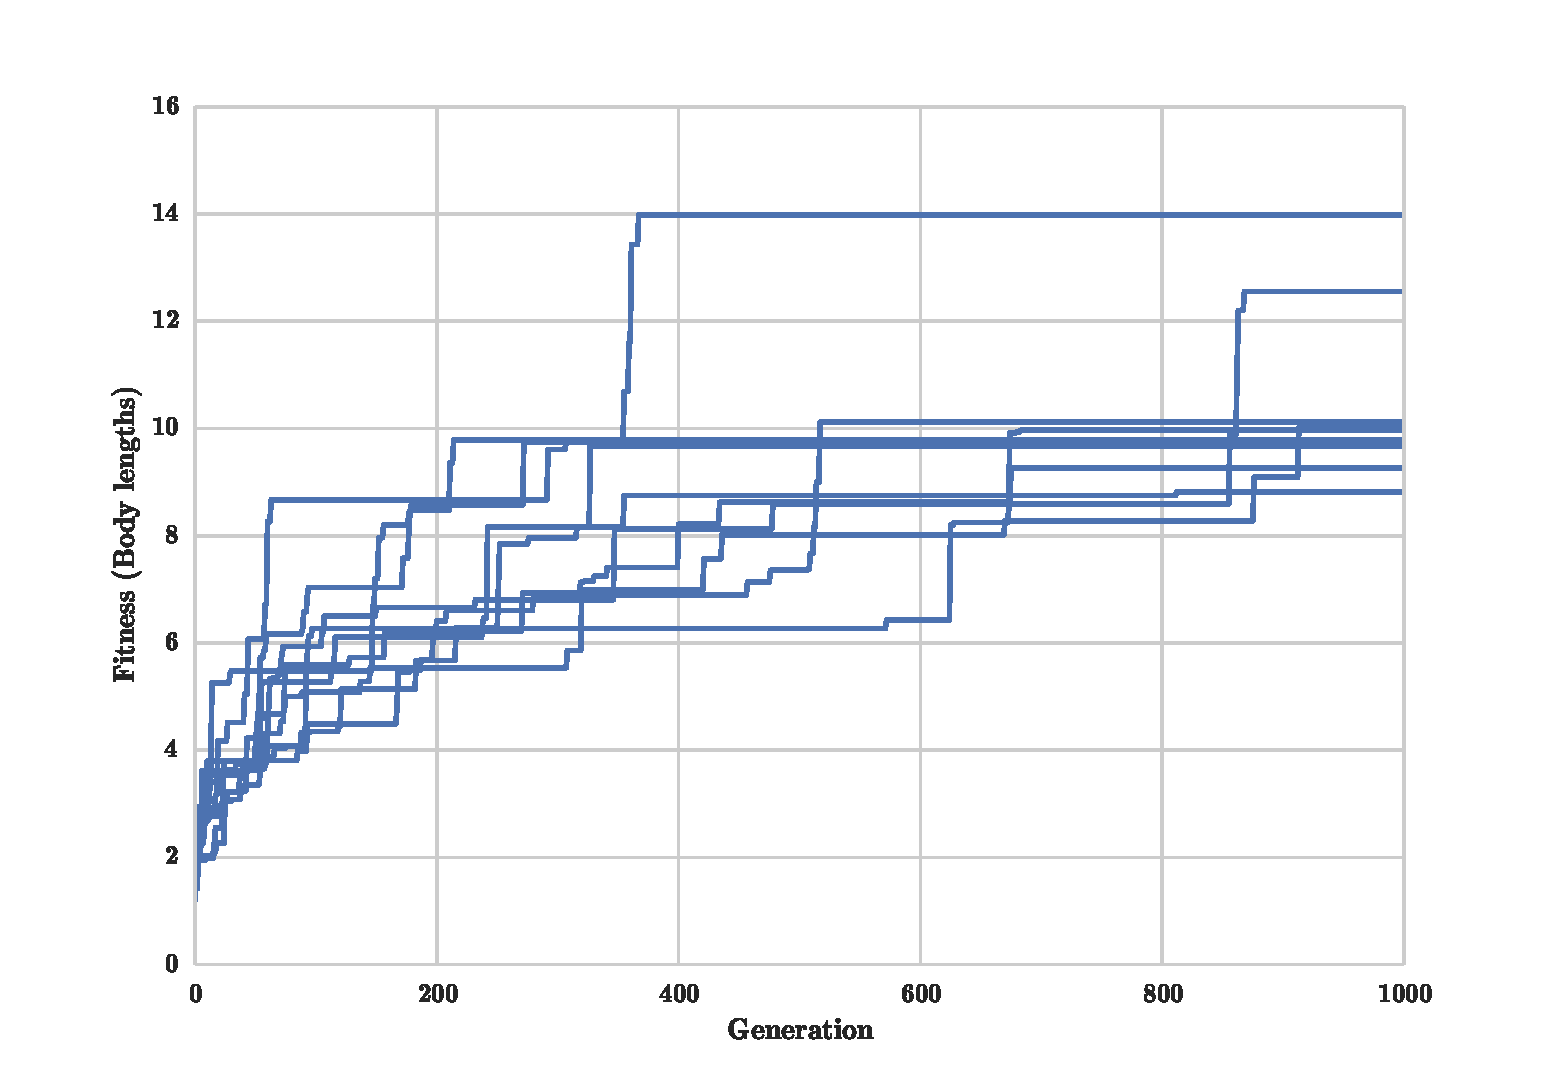
\includegraphics[width=1.0\textwidth]{Figures/Results/indRunsSize10Novelty.pdf}
\caption{Best so far fitness in body lengths displacement of softbot's center of mass from $10$ runs for novelty search. The gravity acceleration for this experiment used was $-27.468\   m/s^2$, the size of the lattice $10\times 10\times10$ and $4$ available materials ($2$-actuated).}
\label{fig:indRunsSize10Novelty}
\end{figure}

\begin{figure}[h!]
\centering
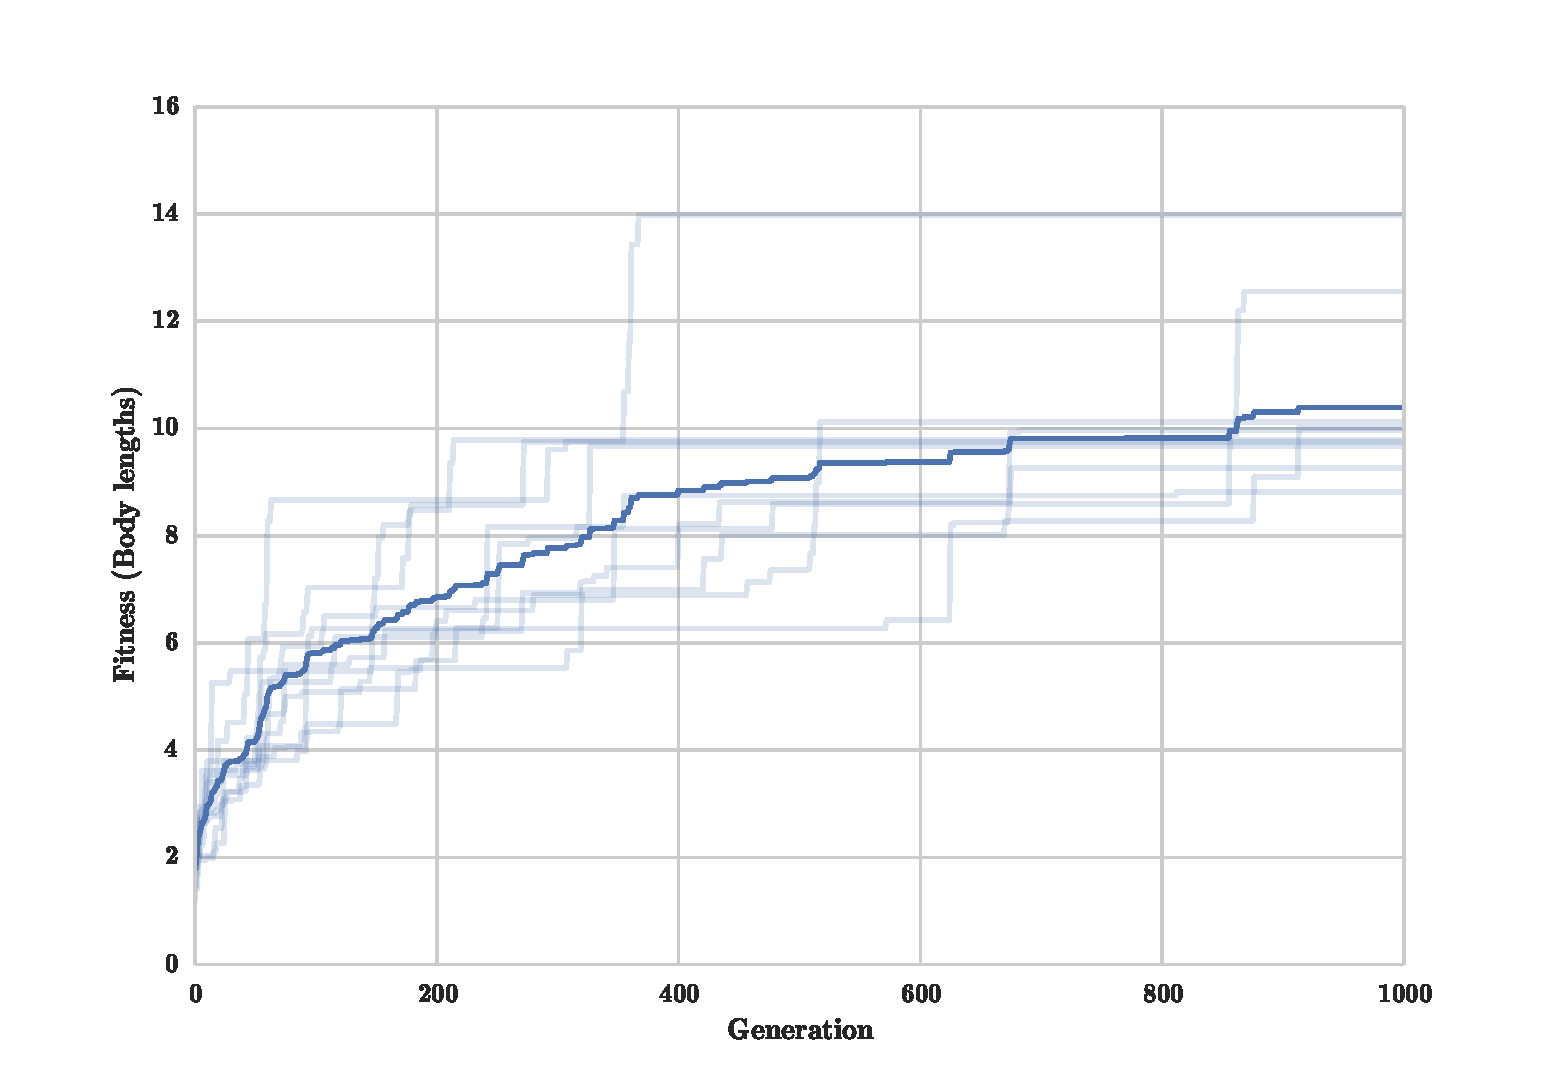
\includegraphics[width=1.0\textwidth]{Figures/Results/indRunnAvgSize10Novelty.pdf}
\caption{Best so far fitness in body lengths displacement of softbot's center of mass from $10$ runs together with their mean (thick line) for novelty search. The gravity acceleration for this experiment used was $-27.468\   m/s^2$, the size of the lattice $10\times 10\times10$ and $4$ available materials ($2$-actuated).}
\label{fig:indRunnAvgSize10Novelty}
\end{figure}


\begin{figure}
\centering
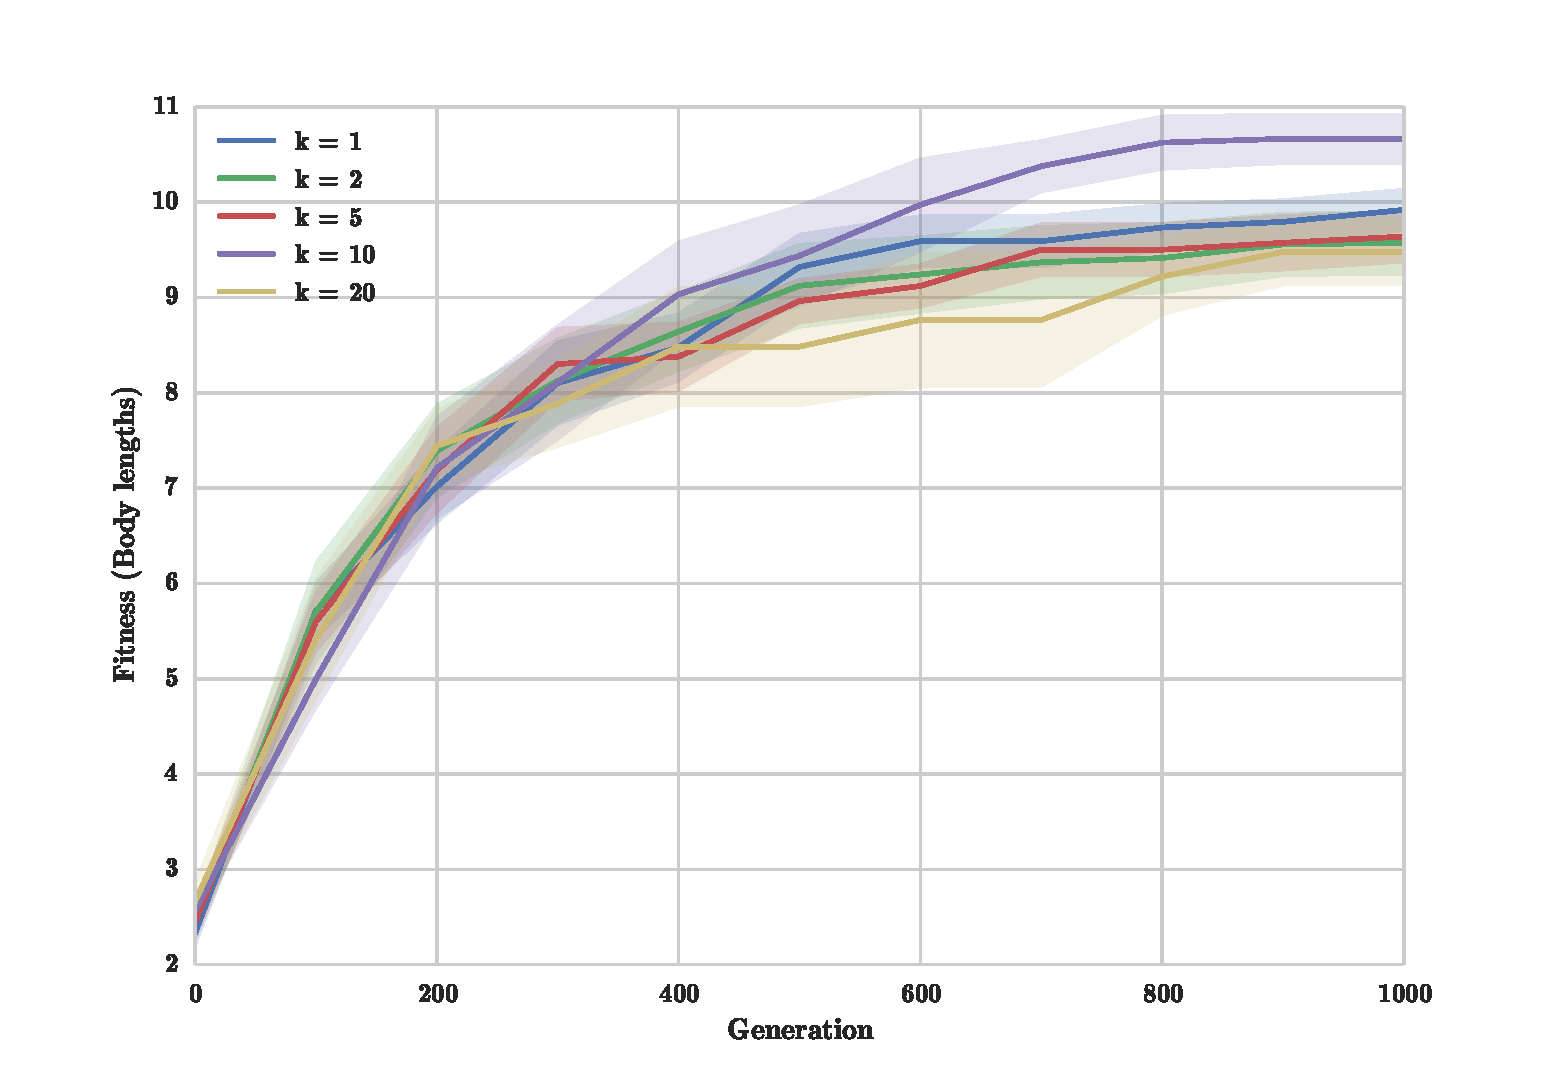
\includegraphics[width=1.0\textwidth]{Figures/Results/KnnExperimentSize5.pdf}
\caption{Novelty search - best so far fitness in body lengths displacement of softbot's center of mass from $10$ runs together with their mean (thick line). The novelty is computed as the average distance from the $K$-nearest behaviors for $K \in \lbrace 1,2,5,10,20 \rbrace $. The gravity acceleration for this experiment used was $-27.468\   m/s^2$, the size of the lattice $5\times 5\times5$ and $4$ available materials ($2$-actuated).}
\label{fig:KnnExperimentSize5}
\end{figure}


















\clearpage
\subsection{Novelty-Fitness Based Search Comparison}

\begin{figure}[h!]
\centering
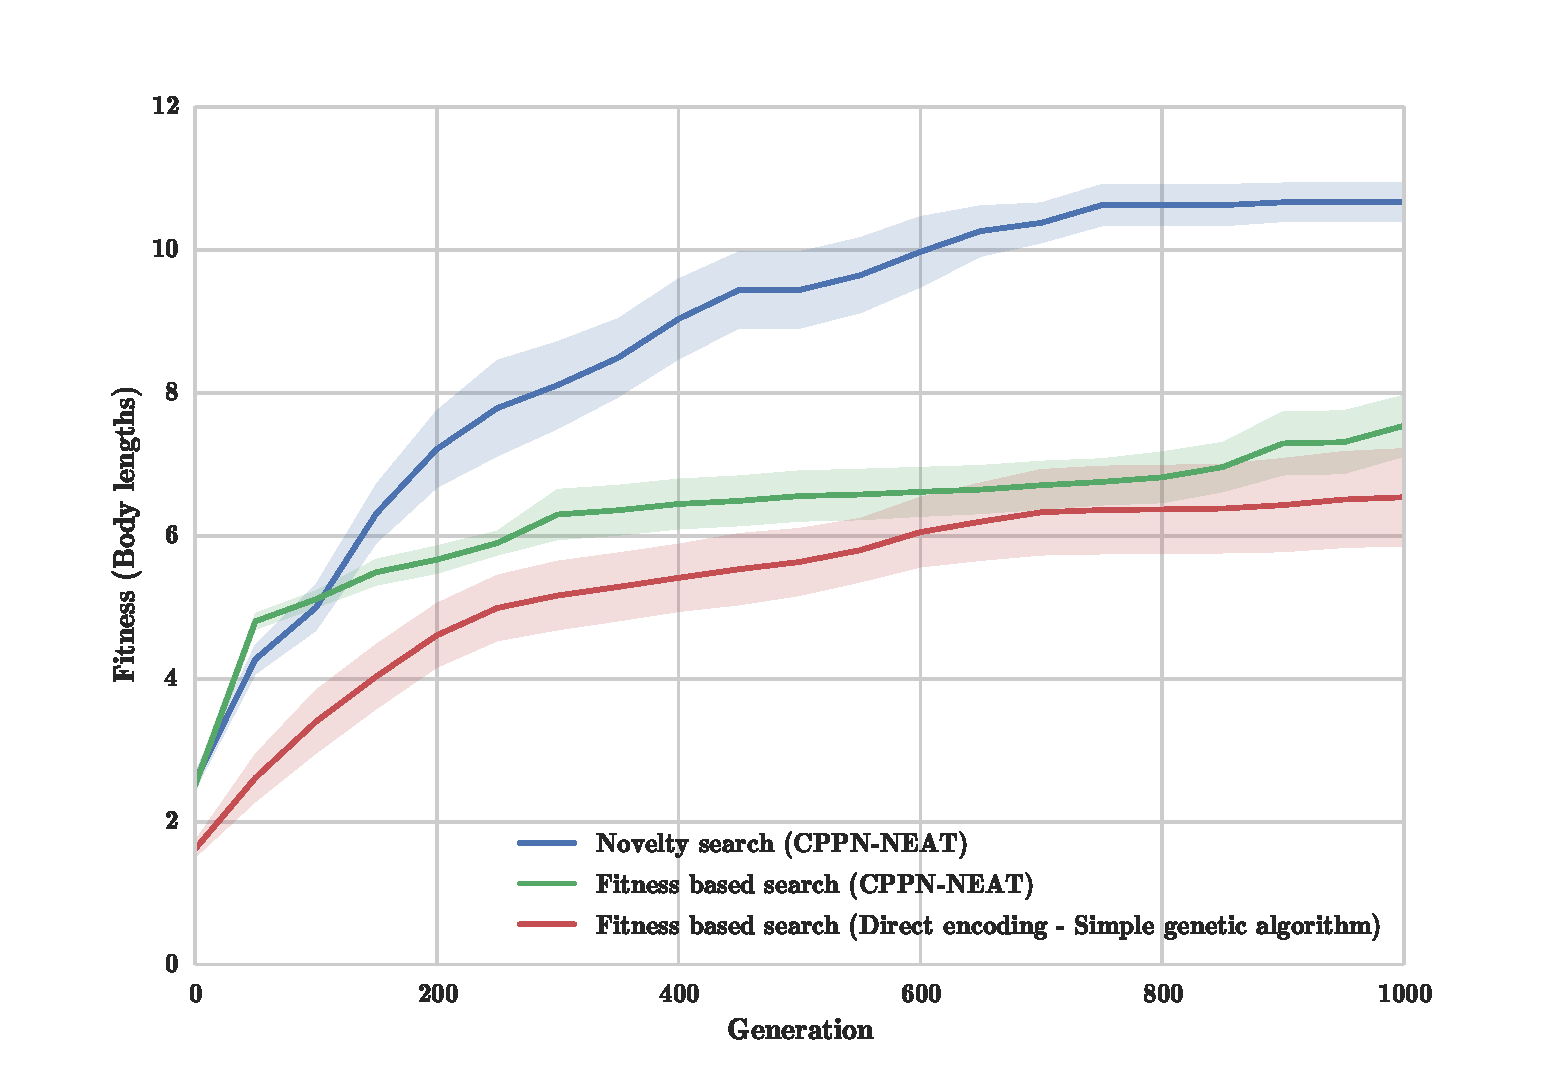
\includegraphics[width=1.0\textwidth]{Figures/Results/FitvsNovVsDirSize5.pdf}
\caption{Best so far fitness in body lengths displacement of softbot's center of mass averaged over $10$ runs together with the standard deviation error. The gravity acceleration for this experiment used was $-27.468\   m/s^2$, the size of the lattice $5\times 5\times5$ and $4$ available materials ($2$-actuated).}
\label{fig:FitvsNovVsDirSize5}
\end{figure}

\begin{figure}[h!]
\centering
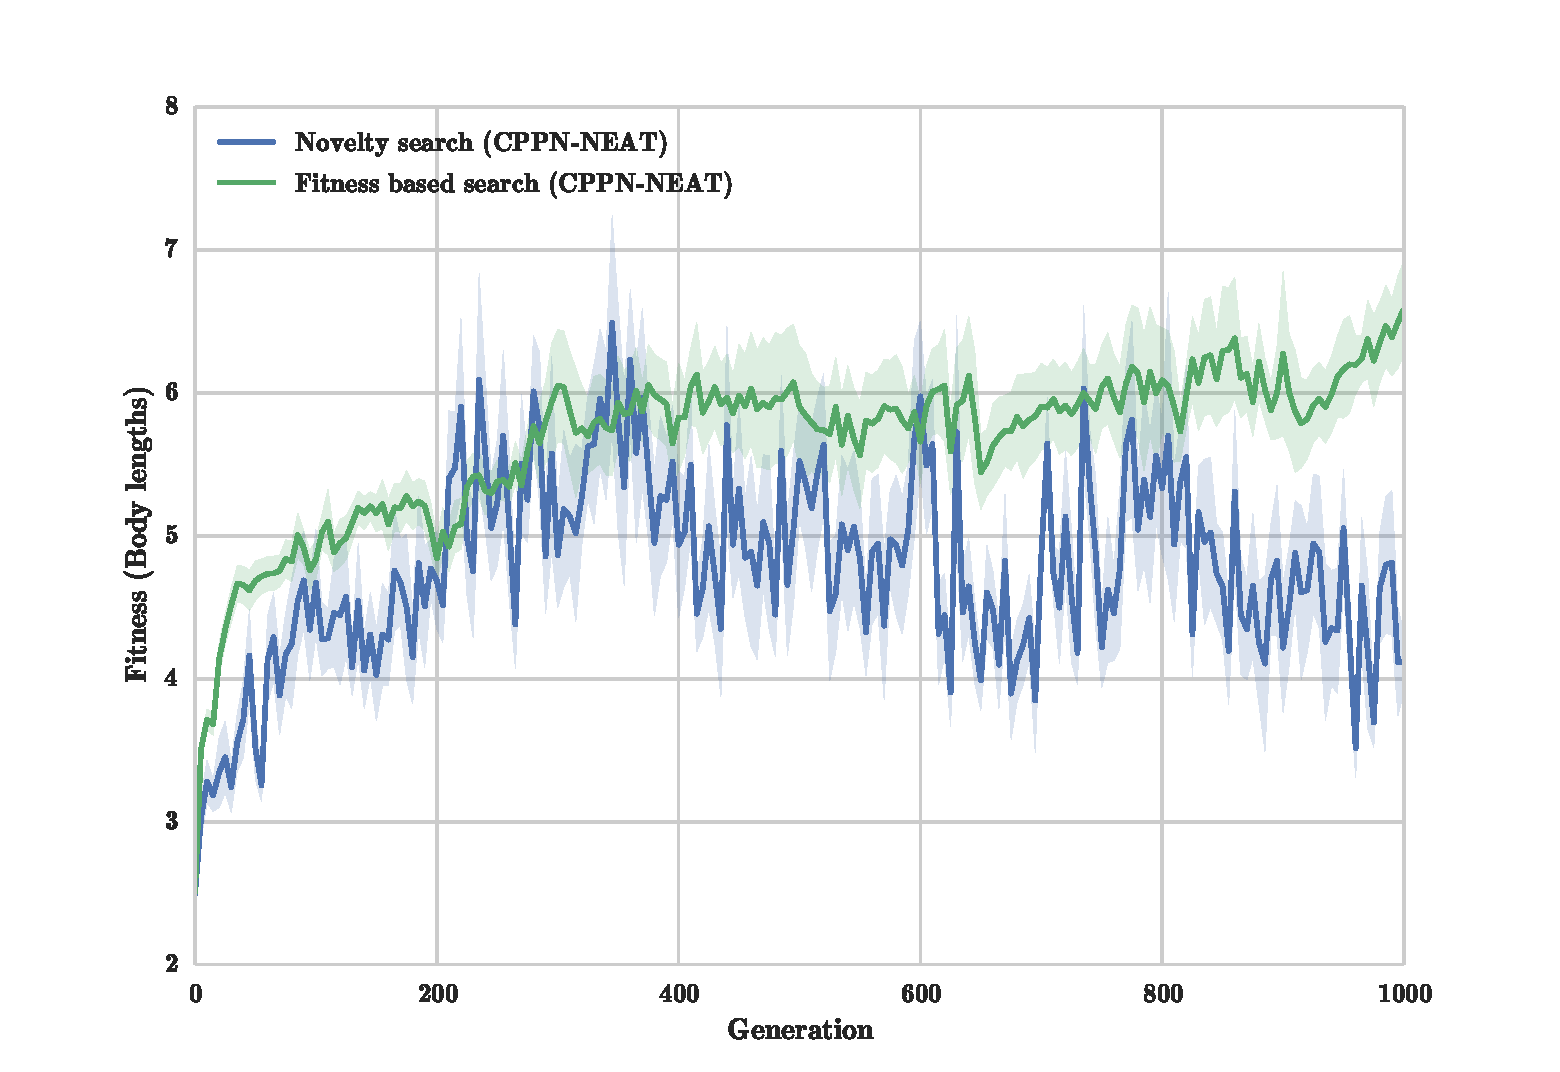
\includegraphics[width=1.0\textwidth]{Figures/Results/AvgGenerChampNoveltyFitnessSize5.pdf}
\caption{Fitness of the generation champion (best individual) per generation in body lengths displacement of softbot's center of mass averaged over $10$ runs together with the standard deviation error. The gravity acceleration for this experiment used was $-27.468\   m/s^2$, the size of the lattice $5\times 5\times5$ and $4$ available materials ($2$-actuated).}
\label{fig:AvgGenerChampNoveltyFitnessSize5}
\end{figure}

\begin{figure}[h!]
\centering
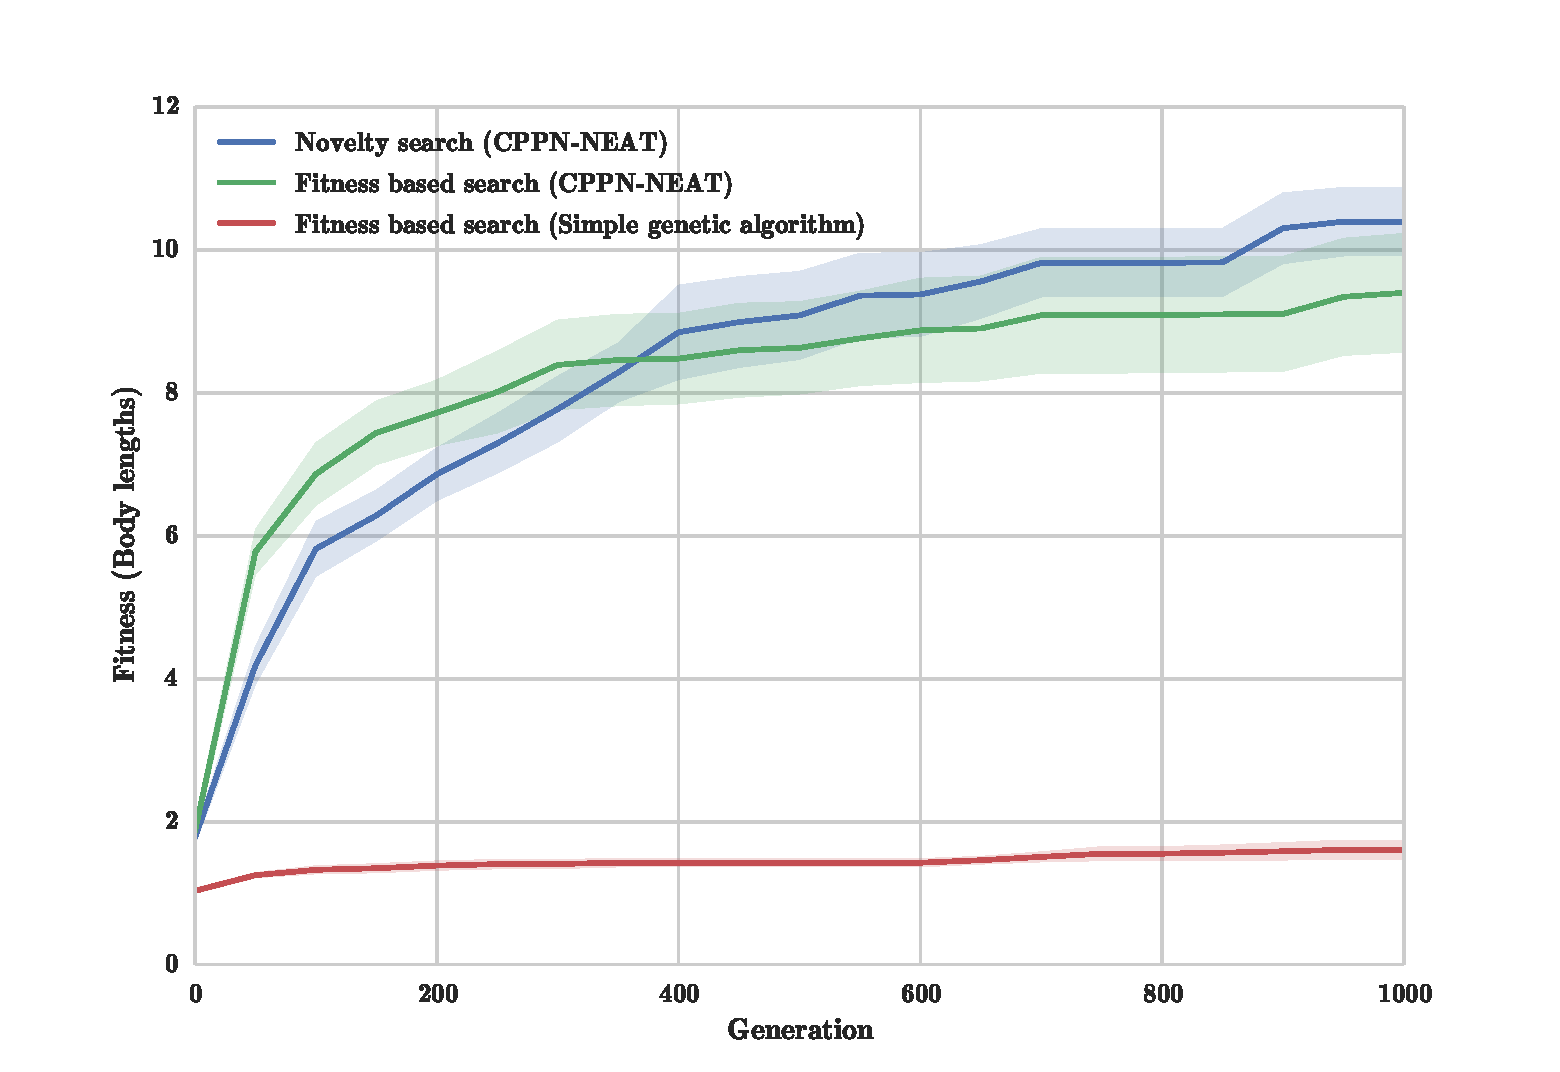
\includegraphics[width=1.0\textwidth]{Figures/Results/FitvsNovVsDirSize10.pdf}
\caption{Best so far fitness in body lengths displacement of softbot's center of mass averaged over $10$ runs together with the standard deviation error. The gravity acceleration for this experiment used was $-27.468\   m/s^2$, the size of the lattice $10\times 10\times10$ and $4$ available materials ($2$-actuated).}
\label{fig:FitvsNovVsDirSize10}
\end{figure}

\begin{figure}
\centering
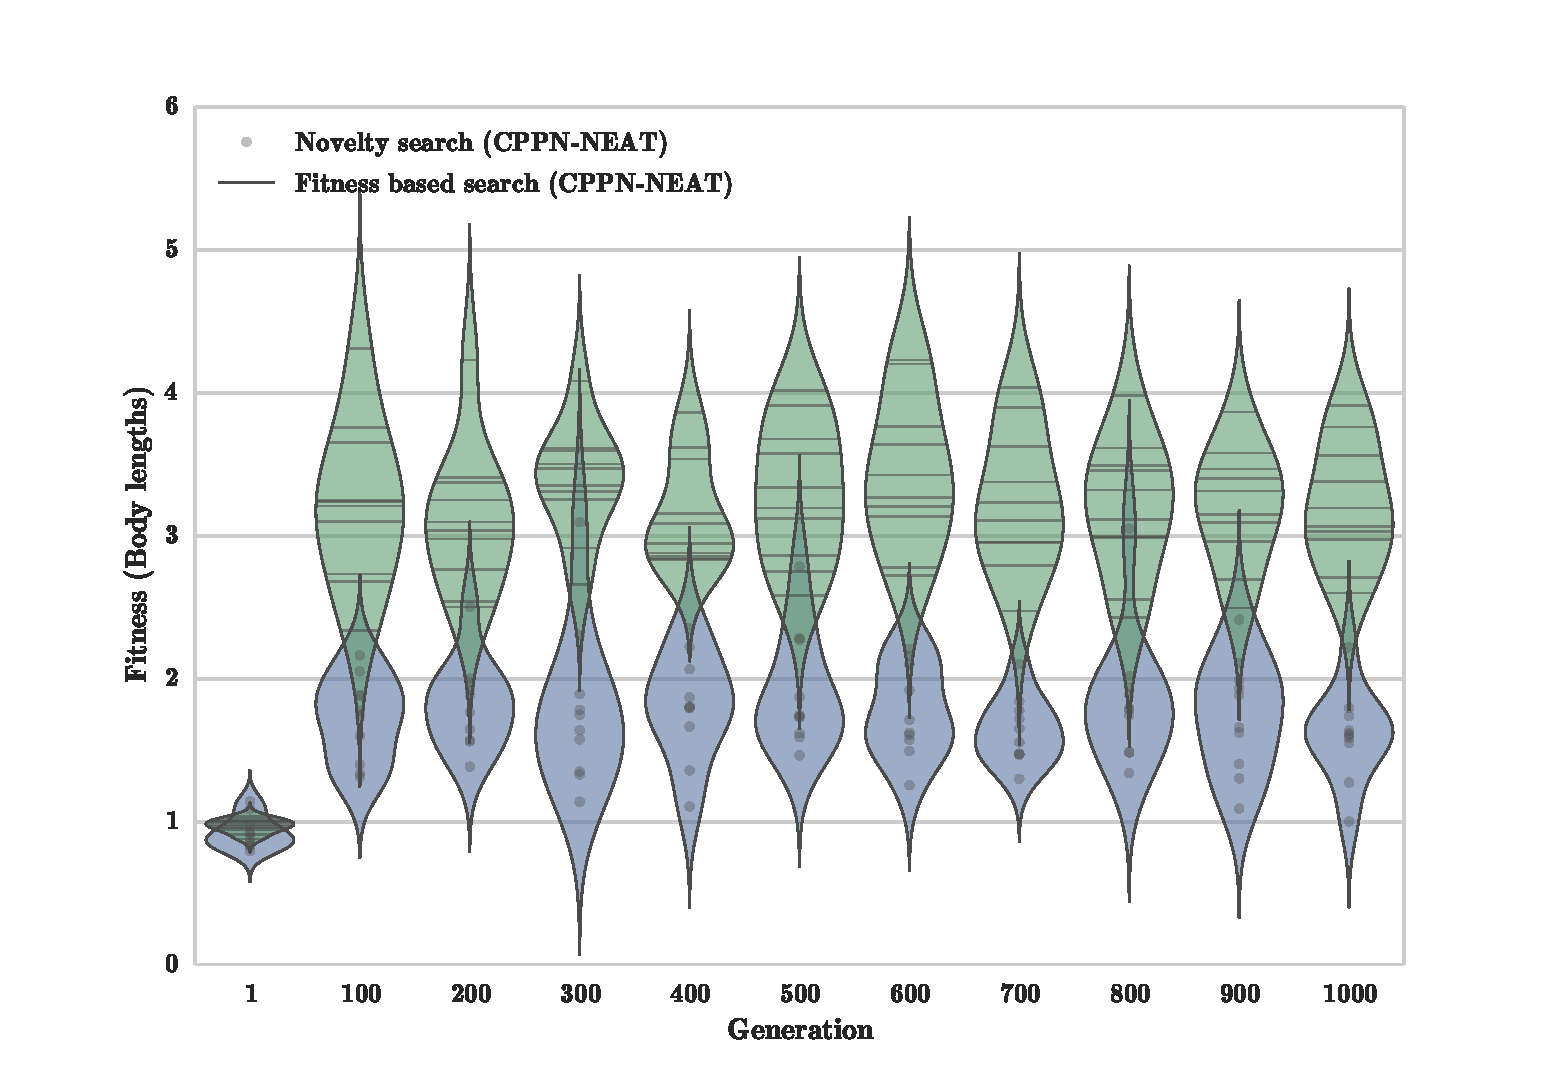
\includegraphics[width=1.0\textwidth]{Figures/Results/ViolinPlotsAvgGenFitSize5.pdf}
\caption{Distributions of average population fitness per generation over 10 runs. The gravity acceleration for this experiment used was $-27.468\   m/s^2$, the size of the lattice $5\times 5\times5$ and $4$ available materials ($2$-actuated). Blue (Novelty search), Green(Fitness based search).}
\label{fig:ViolinPlotsAvgGenFitSize5}
\end{figure}


\begin{figure}
\centering
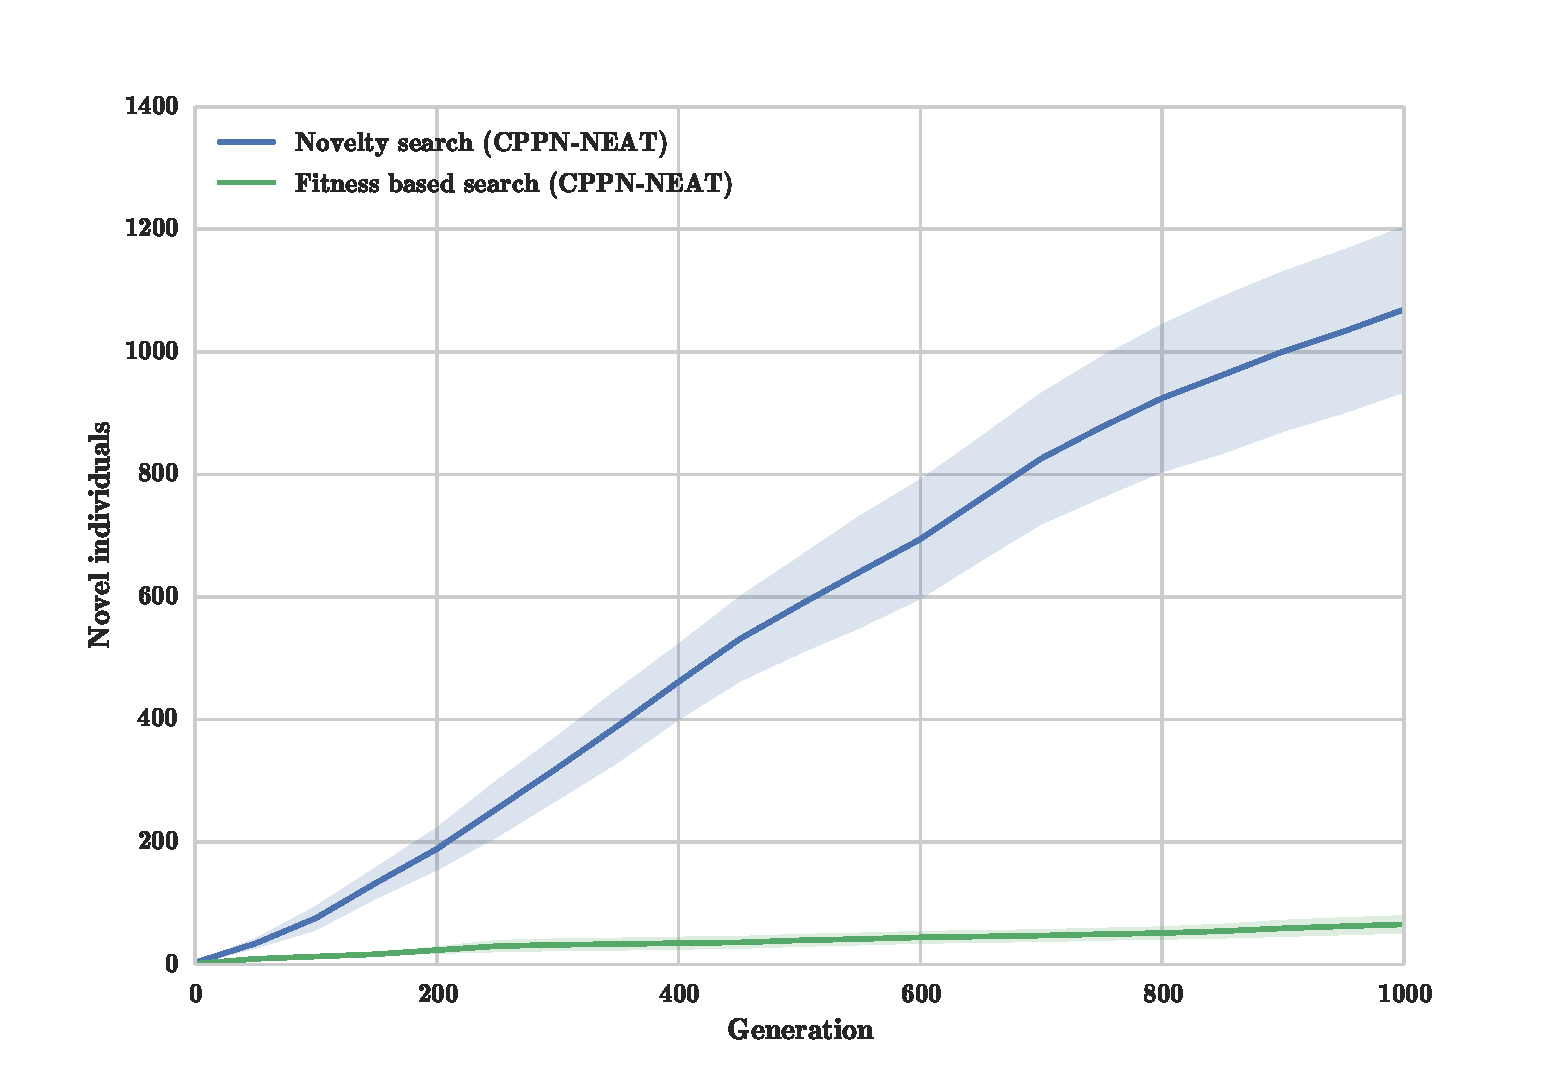
\includegraphics[width=1.0\textwidth]{Figures/Results/novelIndividualsFitNovComp.pdf}
\caption{Novel individual's behaviors upto generation averaged over 10 runs. The novelty is computed as the average distance from the $10$-nearest behaviors. The gravity acceleration for this experiment used was $-27.468\   m/s^2$, the size of the lattice $5\times 5\times5$ and $4$ available materials ($2$-actuated). Blue (Novelty search), Green (Fitness based search).}
\label{fig:ViolinPlotsAvgGenFitSize5}
\end{figure}



\begin{figure}
\centering
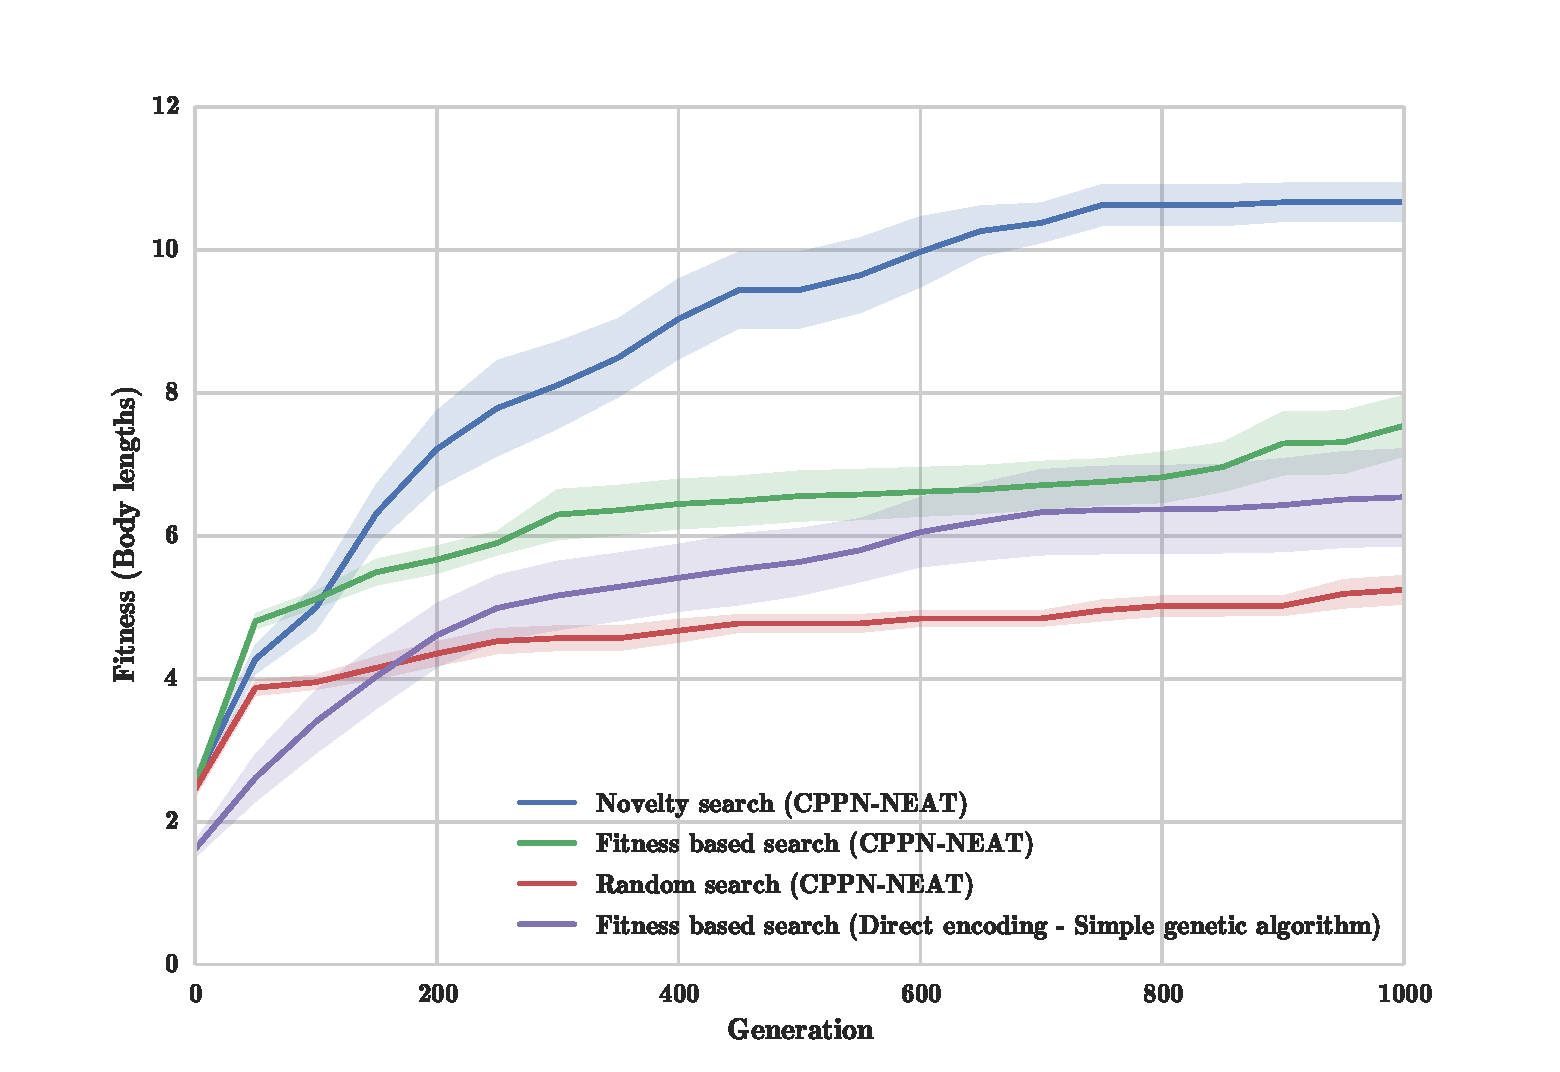
\includegraphics[width=1.0\textwidth]{Figures/Results/FitNovRandomDirectSize5.pdf}
\caption{Best so far fitness in body lengths displacement of softbot's center of mass averaged over $10$ runs together with the standard deviation error. The gravity acceleration for this experiment used was $-27.468\   m/s^2$, the size of the lattice $5\times 5\times5$ and $4$ available materials ($2$-actuated).}
\label{fig:FitNovRandomDirectSize5}
\end{figure}

\begin{figure}
\centering
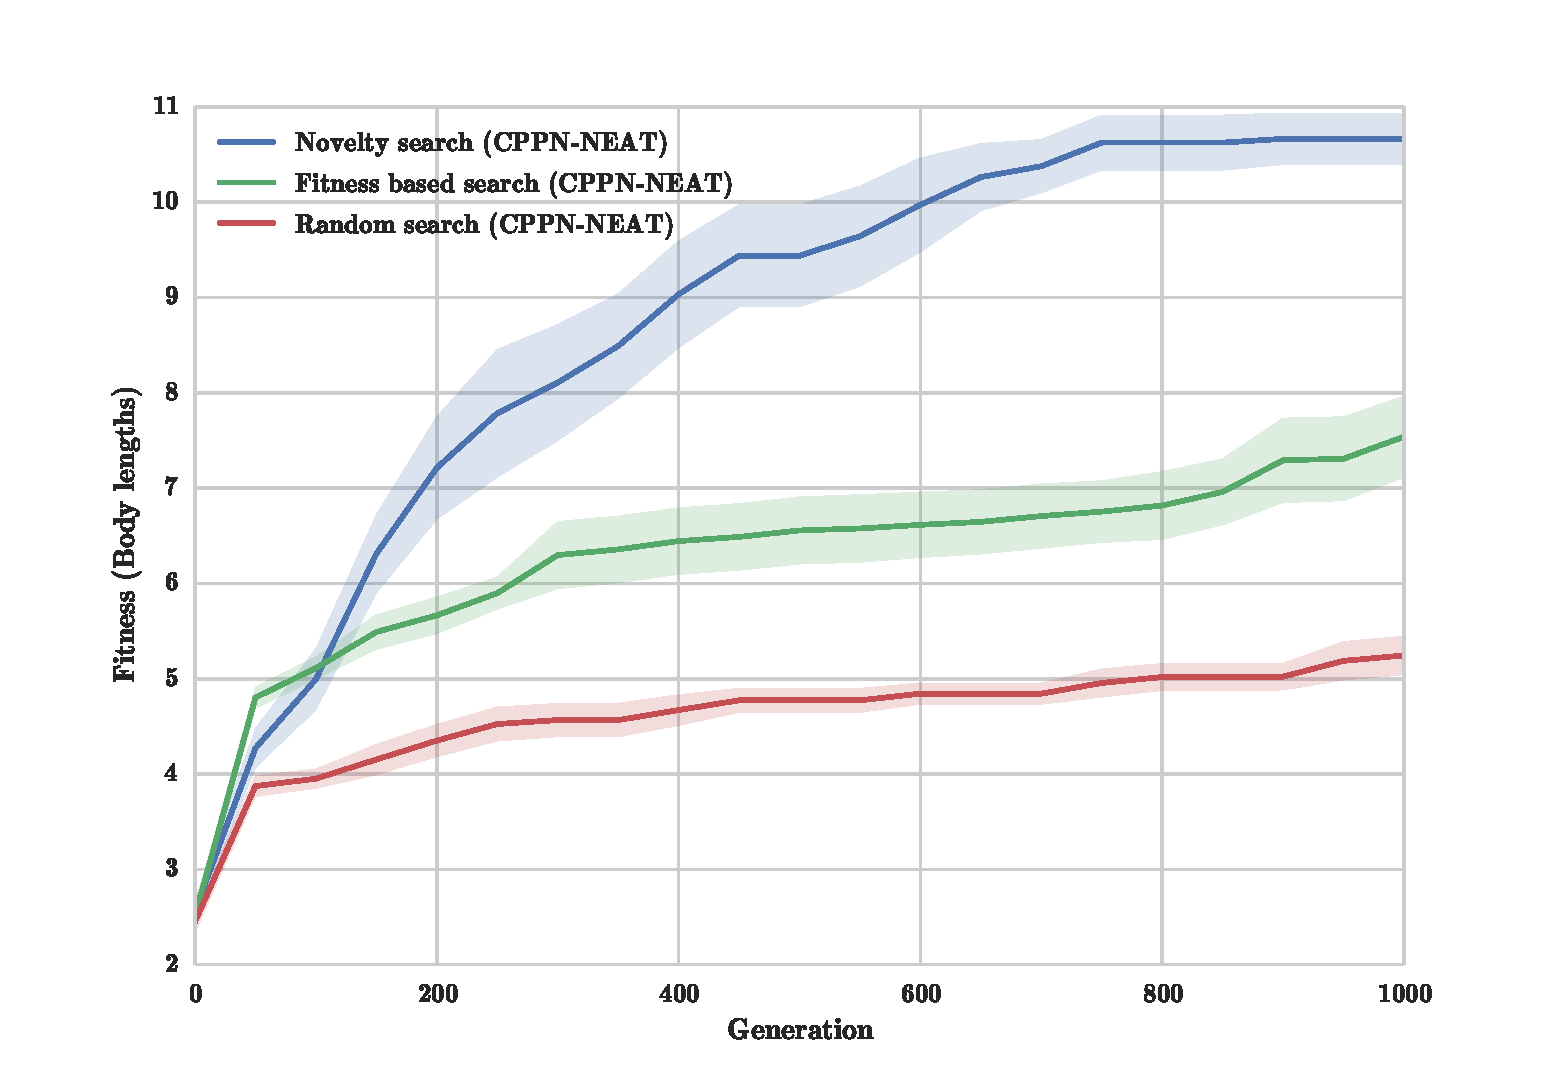
\includegraphics[width=1.0\textwidth]{Figures/Results/FitNovRandomSize5.pdf}
\caption{Best so far fitness in body lengths displacement of softbot's center of mass averaged over $10$ runs together with the standard deviation error. The gravity acceleration for this experiment used was $-27.468\   m/s^2$, the size of the lattice $5\times 5\times5$ and $4$ available materials ($2$-actuated).}
\label{fig:FitNovRandomSize5}
\end{figure}


\begin{figure}
\centering
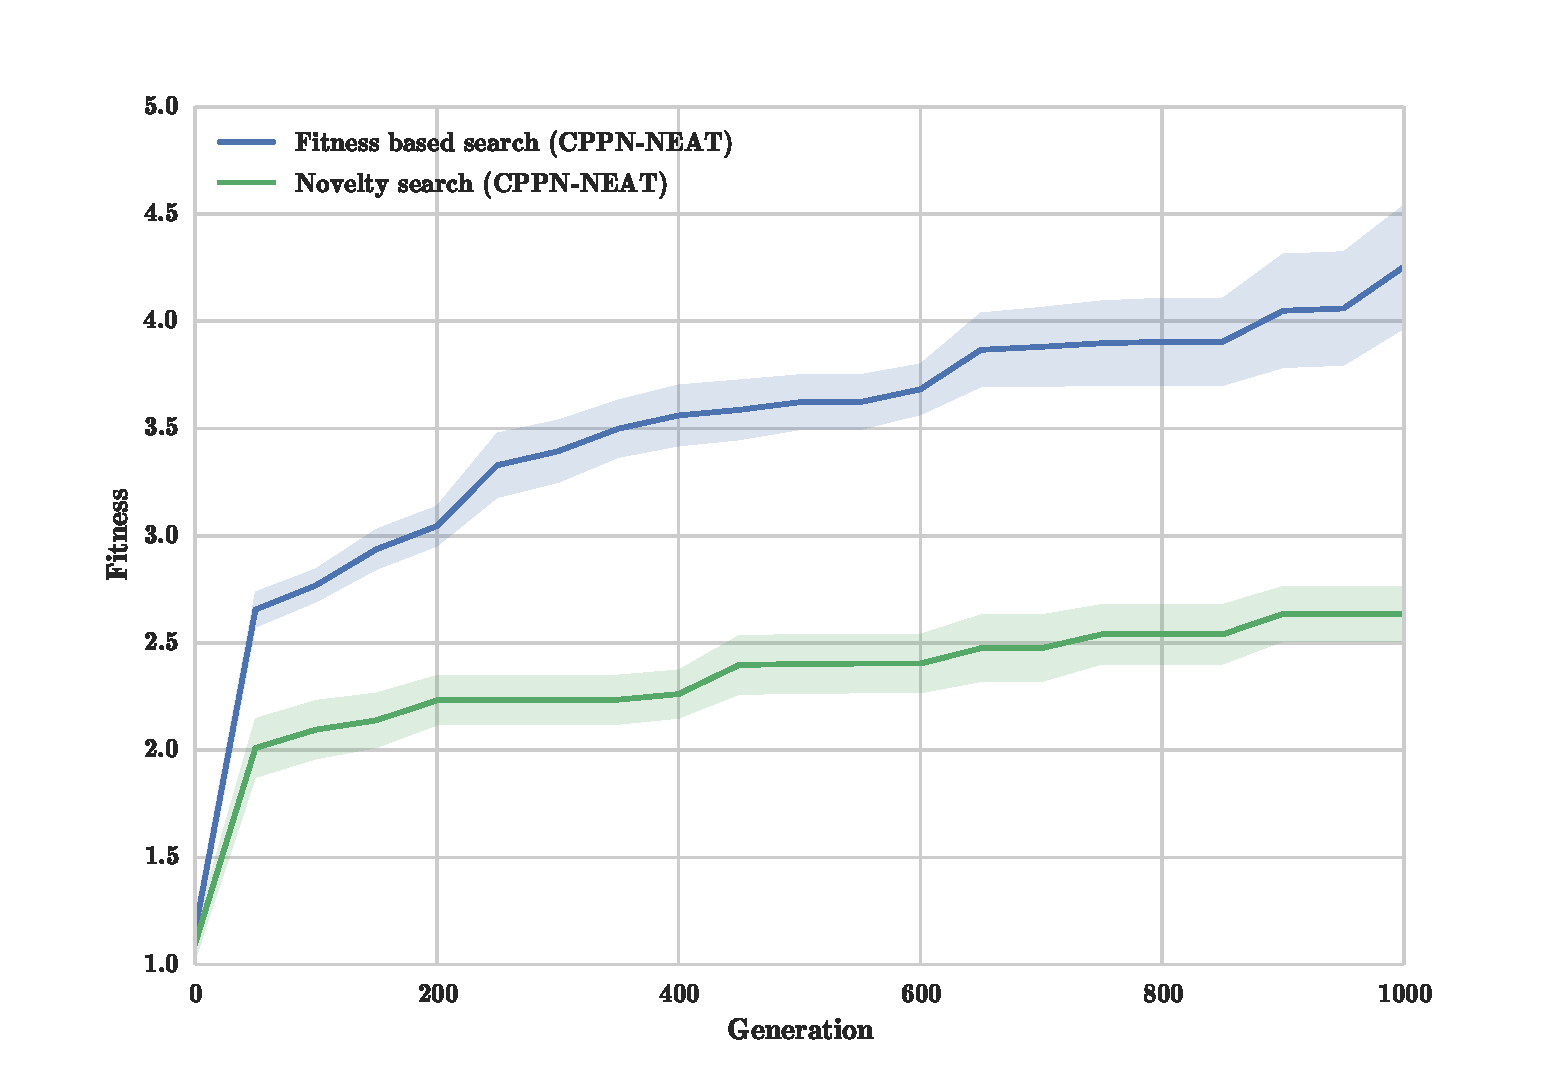
\includegraphics[width=1.0\textwidth]{Figures/Results/FitNovSize5Pen2.pdf}
\caption[]{Best so far fitness averaged over $10$ runs together with the standard deviation error penalizing actuated materials\footnotemark. The gravity acceleration for this experiment used was $-27.468\   m/s^2$, the size of the lattice $5\times 5\times5$ and $4$ available materials ($2$-actuated).}
\label{fig:FitNovRandomSize5}
\end{figure}

\footnotetext{Actuated materials penalize fitness: \[f = (1 - (n_{actuated} / n_{total})^{1.5}) \times disp \], where $n_{actuated}$, is the number of actuated voxels, $n_{total}$ total number of voxels and $disp$ the displacement of the softbot's center of mass.}












\clearpage
\subsection{Local competition in fitness based evolution}

\begin{figure}[h!]
\centering
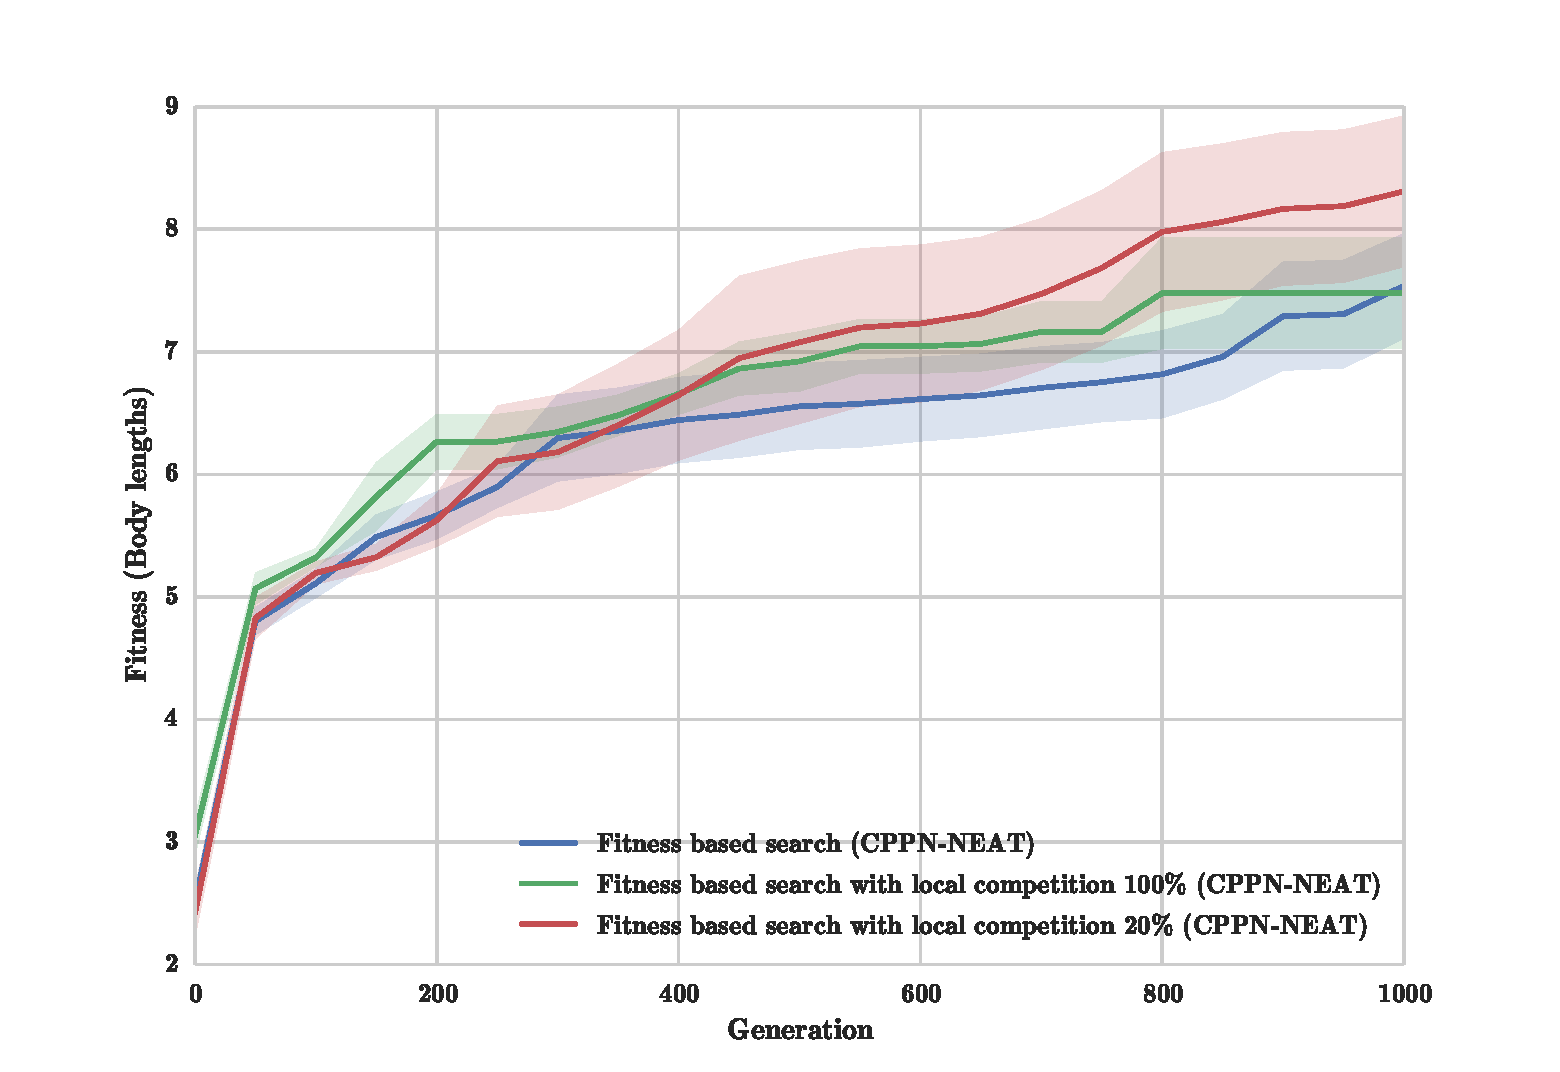
\includegraphics[width=1.0\textwidth]{Figures/Results/fitComp100_20percent.pdf}
\caption{Best so far fitness in body lengths displacement of softbot's center of mass averaged over $10$ runs together with the standard deviation error. Local competition is held among the top $20\%$ and in the complete population of each species. The gravity acceleration for this experiment used was $-27.468\   m/s^2$, the size of the lattice $5\times 5\times5$ and $4$ available materials ($2$-actuated).}
\label{fig:fitComp100_20percent}
\end{figure}

\begin{figure}[h!]
\centering
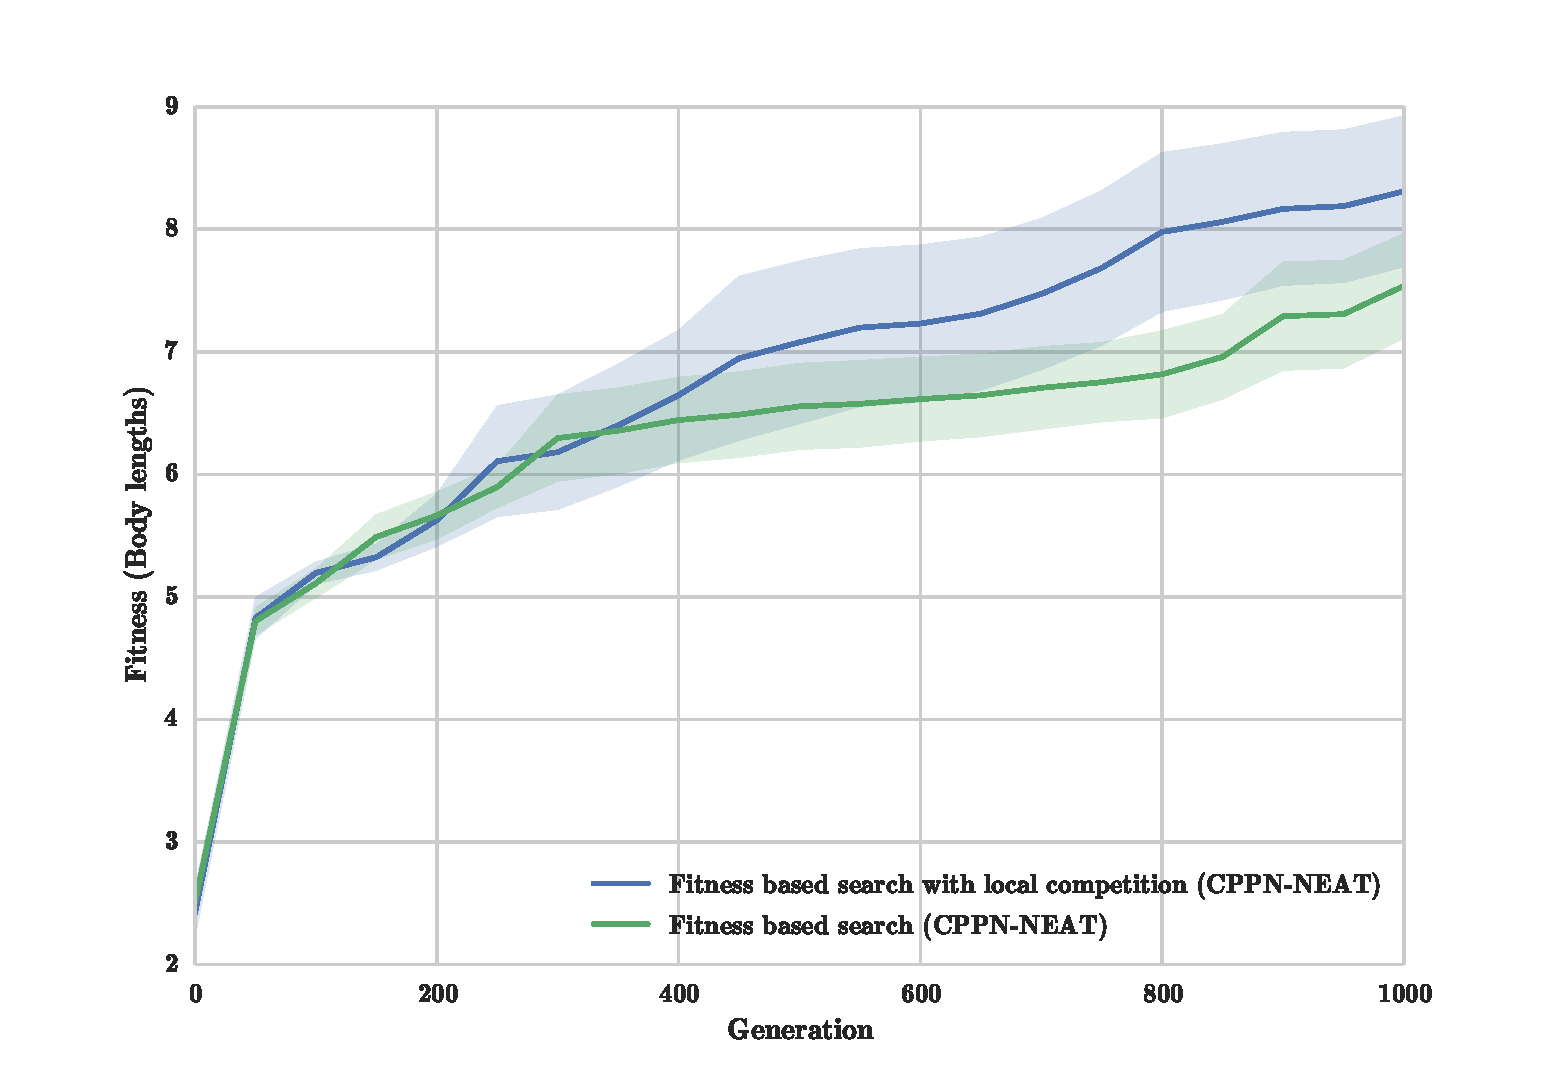
\includegraphics[width=1.0\textwidth]{Figures/Results/FitVsFitCompSize5.pdf}
\caption{Best so far fitness in body lengths displacement of softbot's center of mass averaged over $10$ runs together with the standard deviation error. Local competition is held among the top $20\%$ of each species population. The gravity acceleration for this experiment used was $-27.468\   m/s^2$, the size of the lattice $5\times 5\times5$ and $4$ available materials ($2$-actuated).}
\label{fig:FitVsFitCompSize5}
\end{figure}

\begin{figure}[h!]
\centering
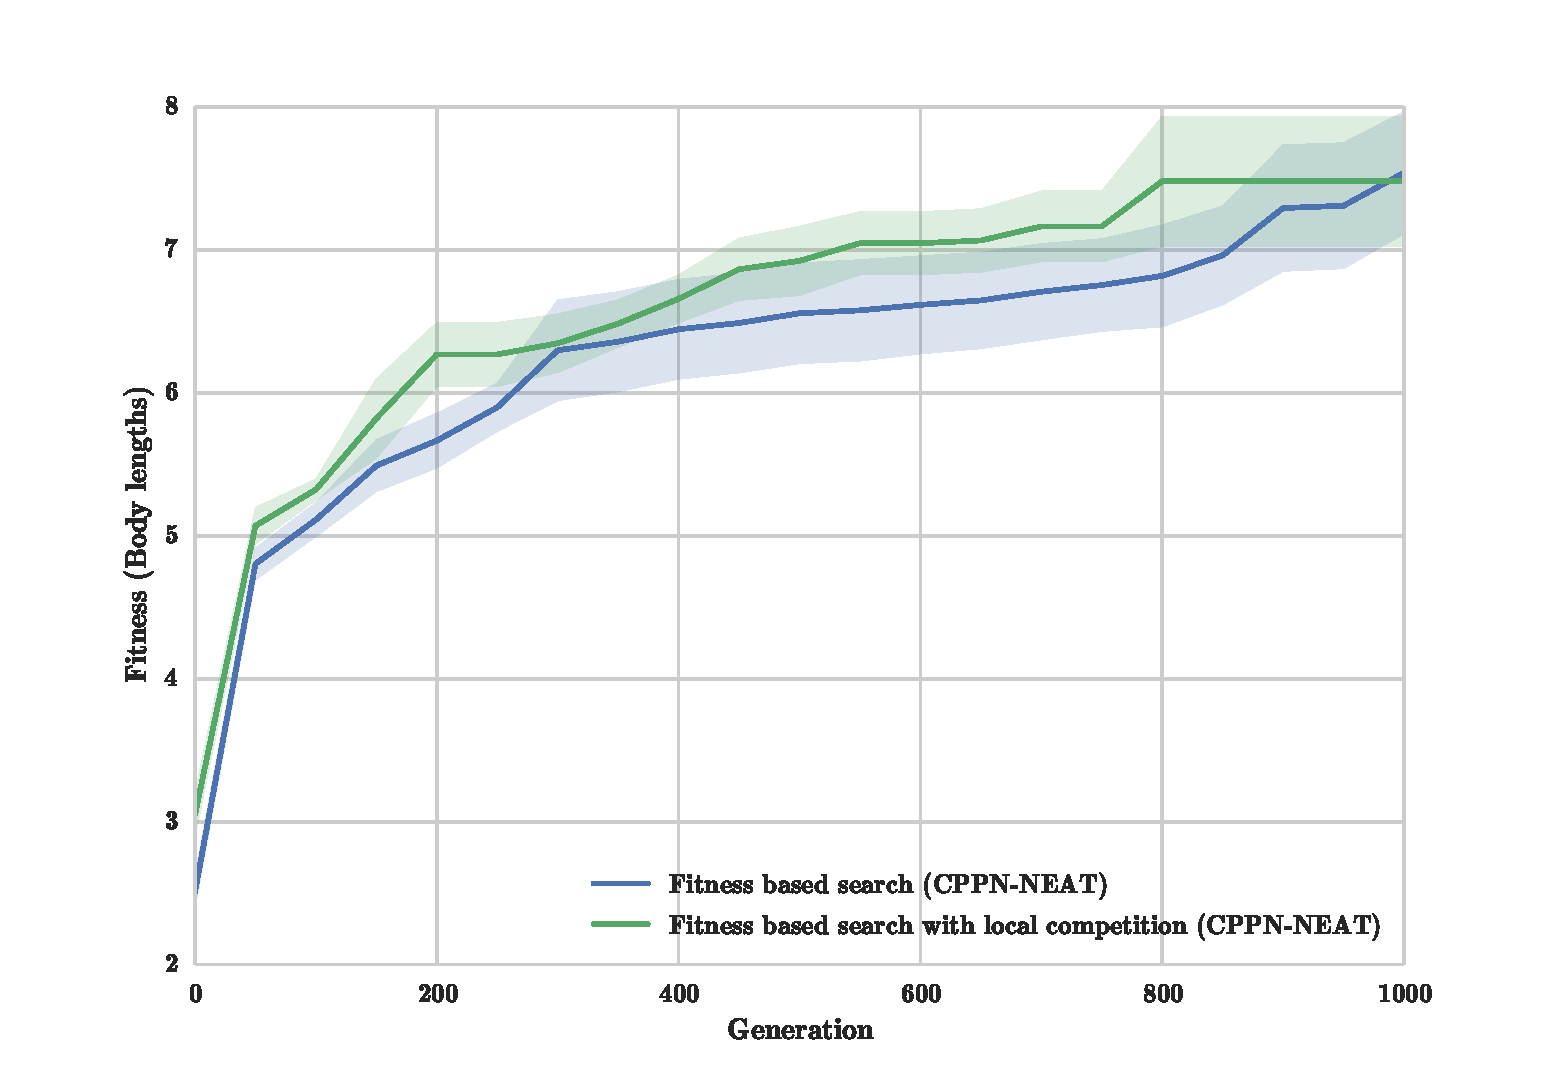
\includegraphics[width=1.0\textwidth]{Figures/Results/fitComp100percent.pdf}
\caption{Best so far fitness in body lengths displacement of softbot's center of mass averaged over $10$ runs together with the standard deviation error. Local competition is held among the complete population of each species. The gravity acceleration for this experiment used was $-27.468\   m/s^2$, the size of the lattice $5\times 5\times5$ and $4$ available materials ($2$-actuated).}
\label{fig:fitComp100percent}
\end{figure}










\clearpage
\subsection{Local competition in novelty search evolution}

\begin{figure}[h!]
{\centering
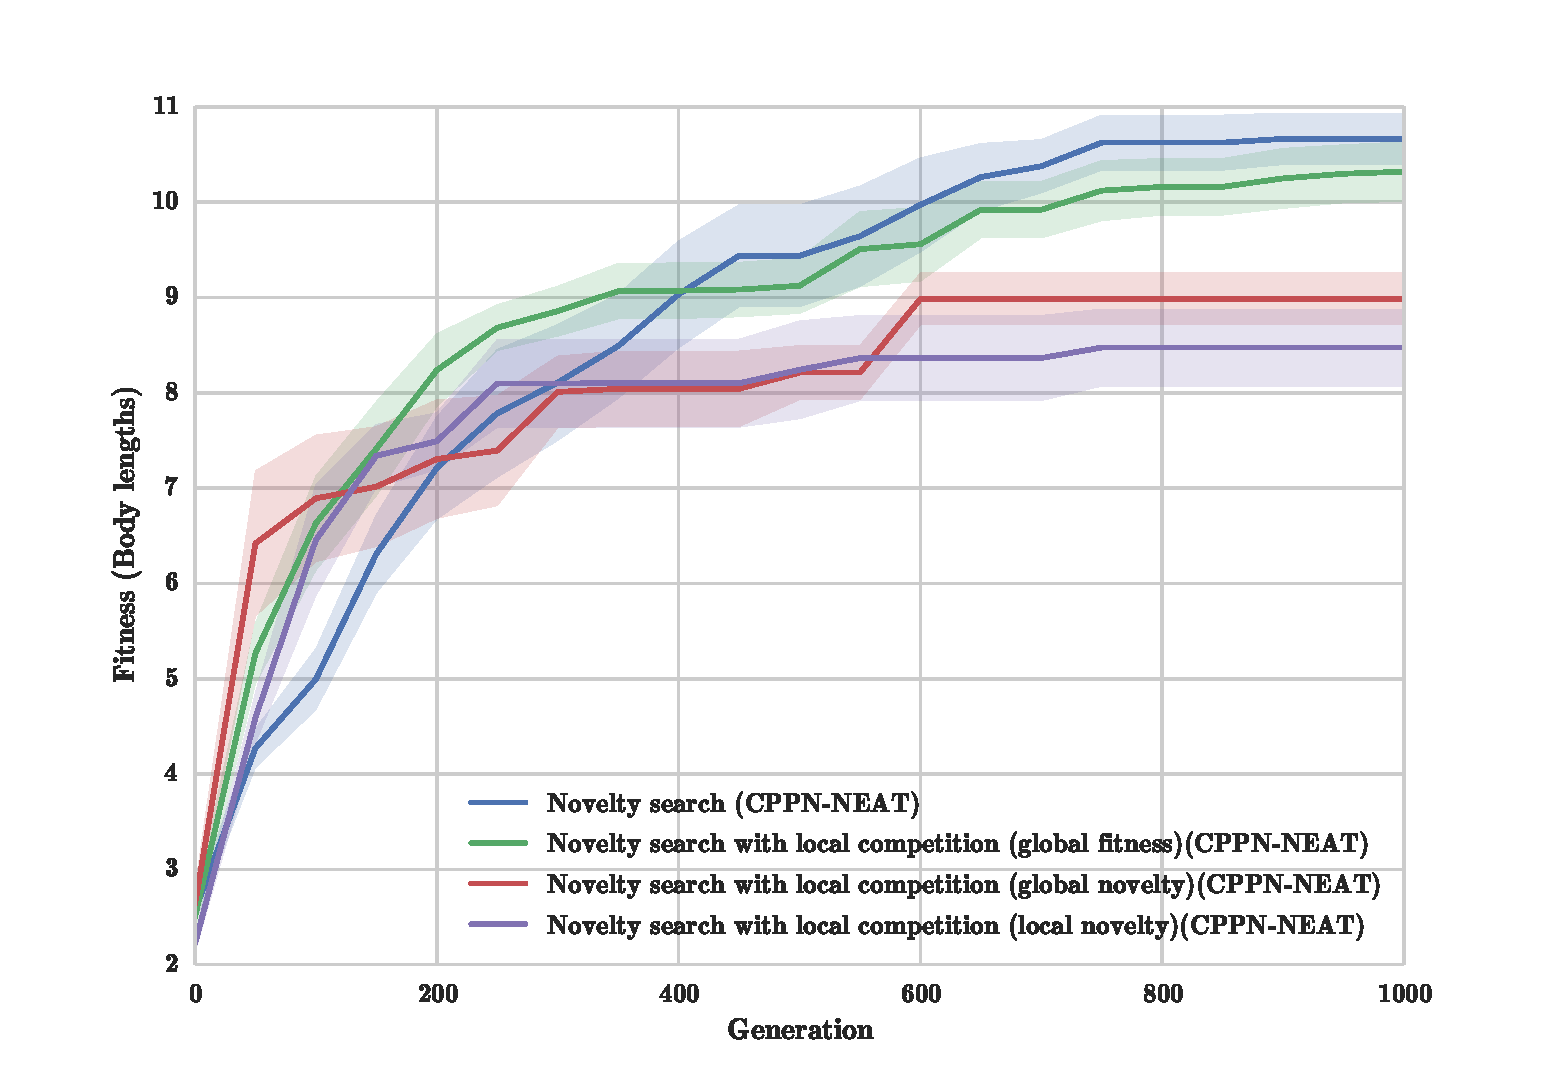
\includegraphics[width=1.0\textwidth]{Figures/Results/NoveltyCompetitionsSize5.pdf}}
\caption{Best so far fitness in body lengths displacement of softbot's center of mass averaged over $10$ runs together with the standard deviation error. Local competition is held among the complete population of each species. The gravity acceleration for this experiment used was $-27.468\   m/s^2$, the size of the lattice $5\times 5\times5$ and $4$ available materials ($2$-actuated).}
\label{fig:NoveltyCompetitionsSize5}
\end{figure}
% Chapter 4

\chapter{Method} % Main chapter title

\label{Method} % For referencing the chapter elsewhere, use \ref{Chapter1} 

\lhead{Chapter 4. \emph{Method}} % This is for the header on each page - perhaps a shortened title

In this chapter, an introduction to the problem specifications this thesis is concerning about, as well as, comprehensive documentation about the methods used, are given.


\section{Problem Introduction}

Recent work in evolutionary robotics shows that evolving the morphologies of soft robotics is possible through compositional pattern producing networks coupled with NEAT evolutionary algorithm. VoxCad simulator provides a test-bench for analyzing soft robot bodies that can be actuated through environmental changes, in this case the temperature. In addition to that, recent work by~\cite{cheney2013unshackling}, shows that very interesting morphologies can be evolved by the CPPN-NEAT algorithm in this kind of soft-robot simulation environment.

\paragraph*{VoxCad}~\\
As far as the simulation settings are concerned, it is not of interest for this thesis to explore the best  not only environmental but also material settings for the evolved soft-robots. For the simulation of the soft material bodies, VoxCad's underlying physics engine \emph{Voxelyze} was used as a stand-alone software to analyze the soft structures without rendering them. Table~\ref{VoxelyzeSimulationSettings}, describes and presents the values used in different variables of the simulation.



\paragraph*{Materials}~\\

\begin{figure}
\centering
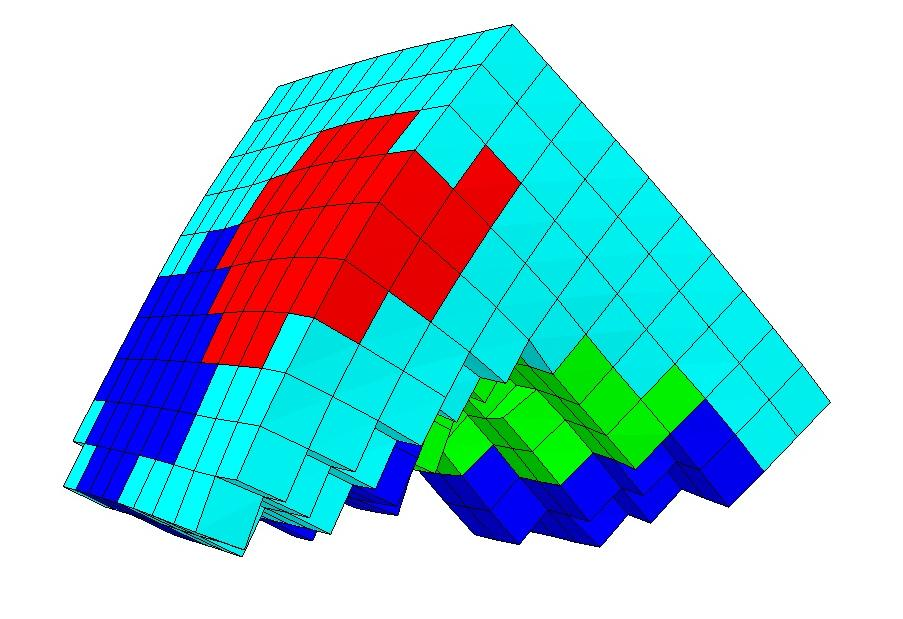
\includegraphics[height=0.2\textheight]{../Figures/Misc/allSoftMaterials.png}
\caption{Soft robot uses four materials (two active, two passive), morphology evolved penalizing actuated materials.}
\label{fig:allSoftMaterials}
\end{figure}

Figure~\ref{fig:allSoftMaterials}, illustrates a soft robot consisting of all four materials used in the experiments. \textcolor{Red}{Red} and \textcolor{Green}{Green} are the only actuated materials with non-zero and opposite thermal expansion coefficients, meaning that their phase in respect to the actuation from temperature changes is equal to half a circle, green voxels contract the same time red expand and vice versa, mimicking living organisms' muscle tissue. The two additional materials represent soft non-actuated tissue that can be soft (soft tissue) or hard (bones). \textcolor{Cyan}{Cyan} voxels are soft, having five times smaller elastic modulus of their material than \textcolor{Blue}{Blue} which have $50$ \texttt{MPa}.


\section{Direct-Generative Random Soft-Robots}
To evaluate all the following methods, information about the performance of random generated morphologies must be present. In order to achieve that, two random approaches which will also help the understanding between direct and indirect coding implemented. Direct coding which is a straightforward encoding scheme assigns randomly the presence of a voxel in a lattice's coordinate, if a voxel will be created then it will be assigned a random material from the palette. The probability of adding a voxel is $0.5$, after all voxels have been assigned a material, unconnected parts of of the structure will be removed, keeping only the largest connected structure in the lattice.


\begin{figure}
\centering
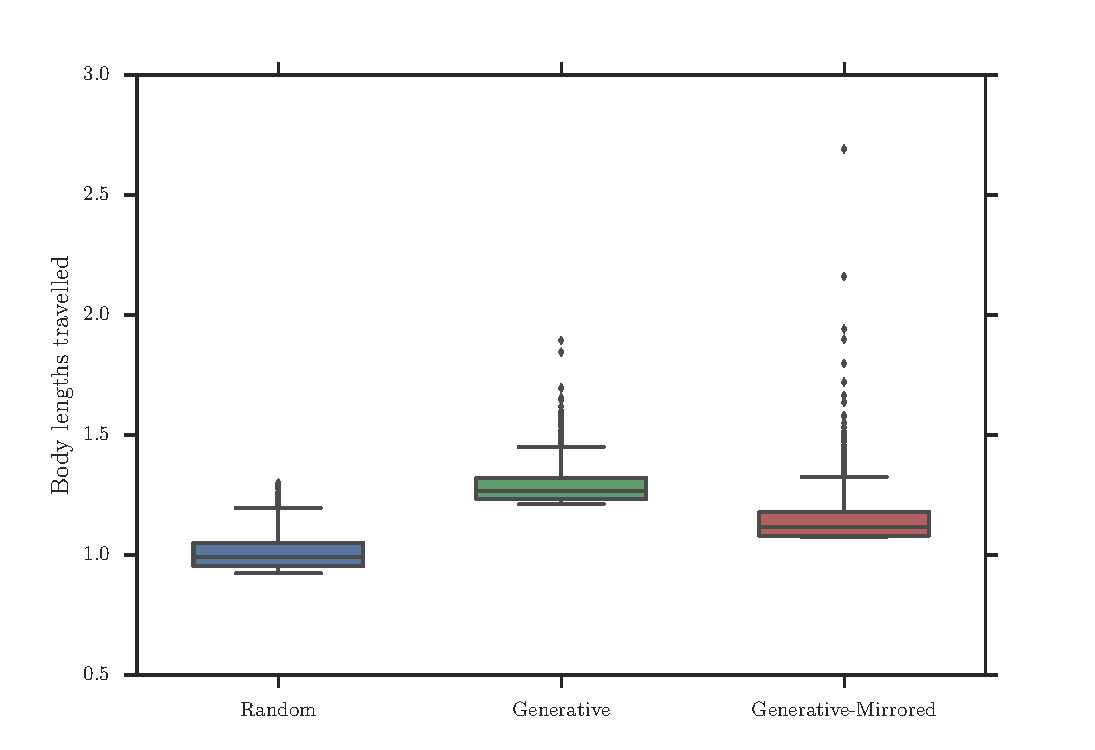
\includegraphics[width=1.0\textwidth]{../Figures/Results/random.pdf}\\
\hspace{0.1cm}
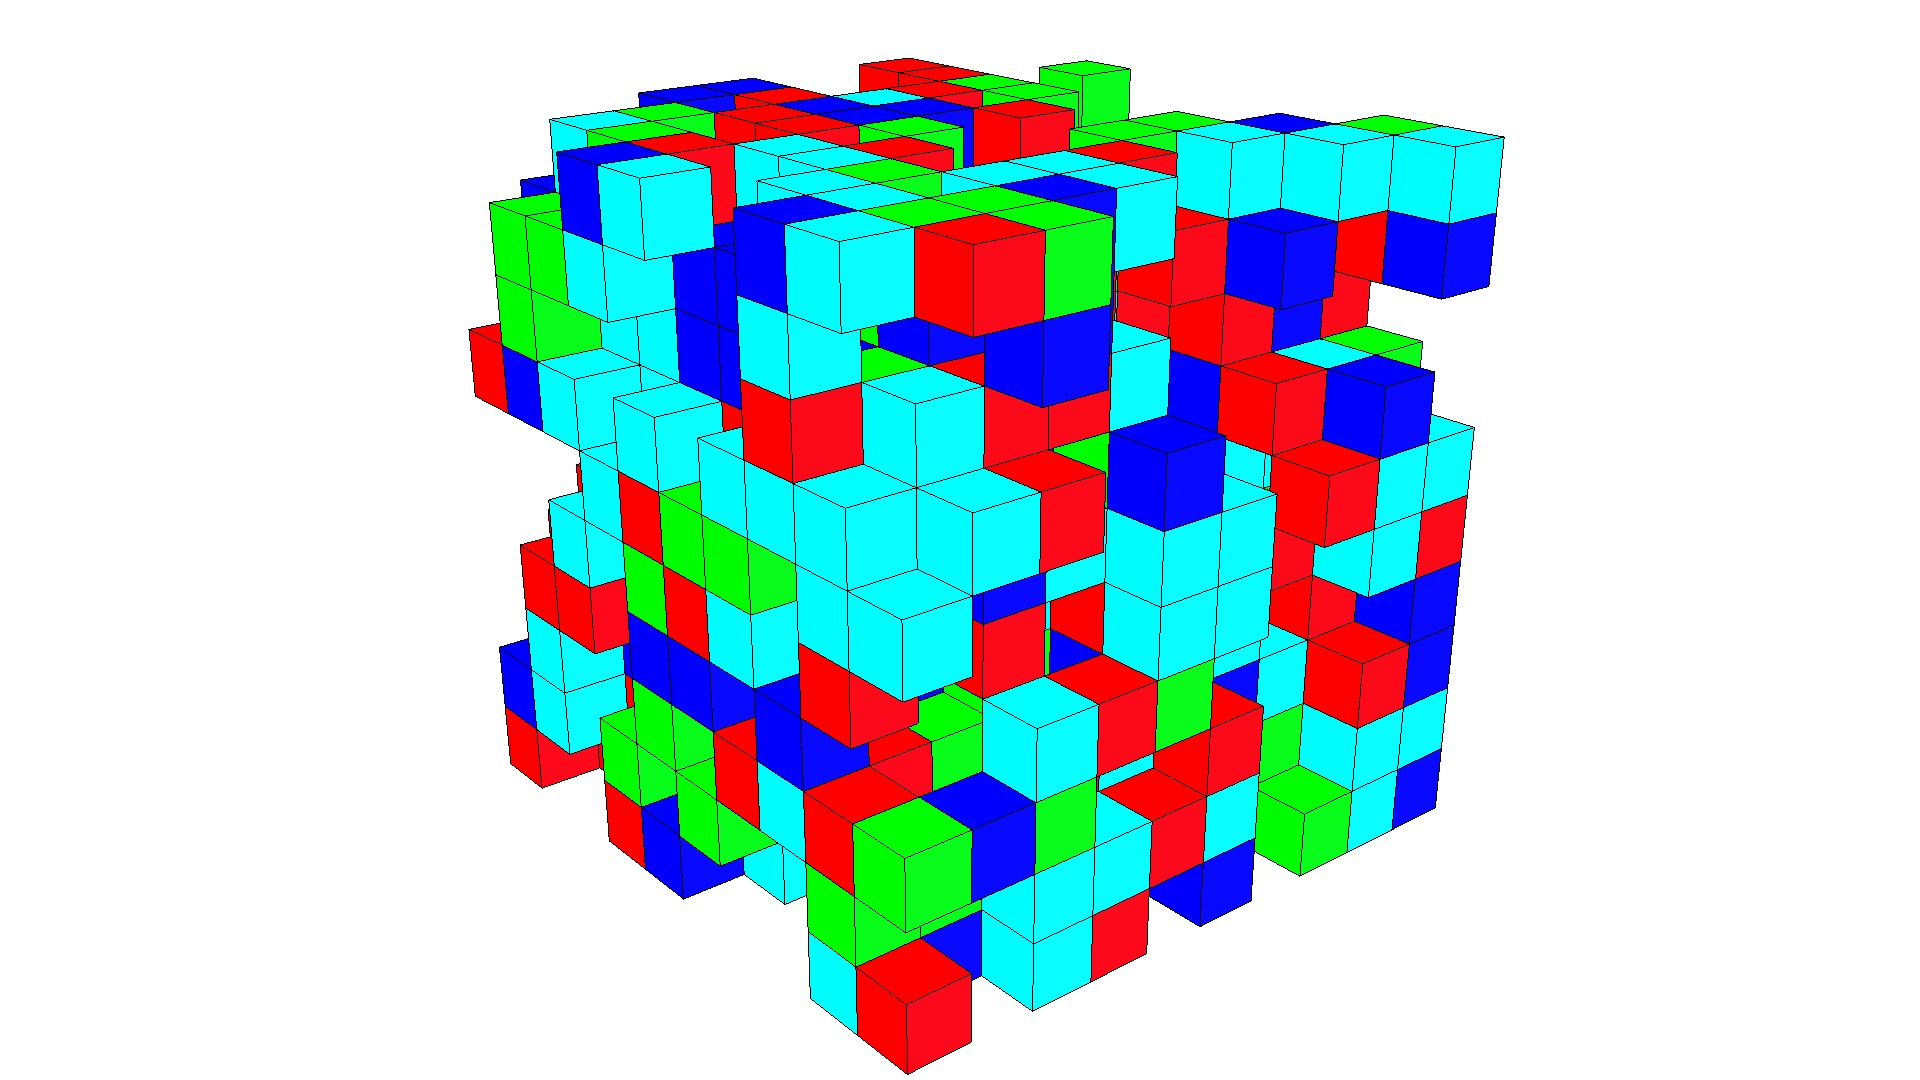
\includegraphics[height=0.15\textwidth]{../Figures/Robots/random.jpg}
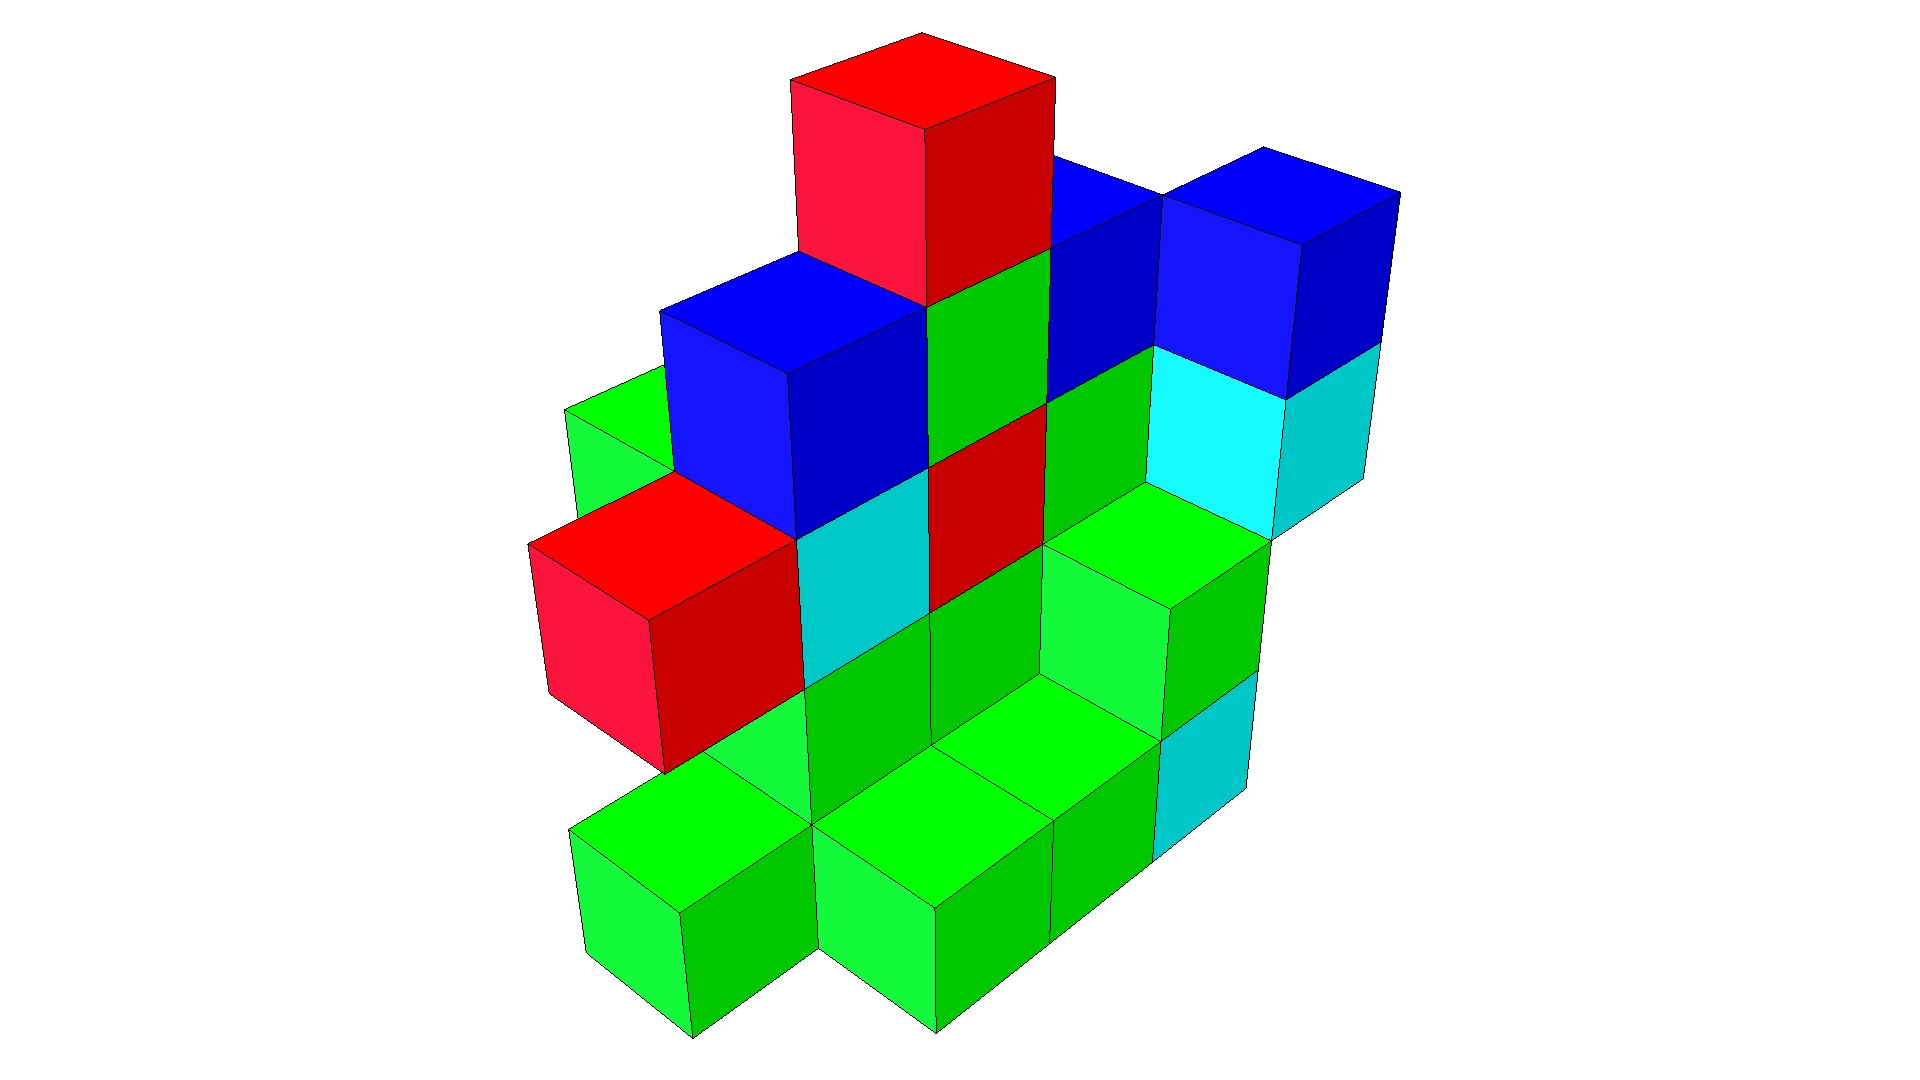
\includegraphics[height=0.15\textwidth]{../Figures/Robots/rg0.jpg}
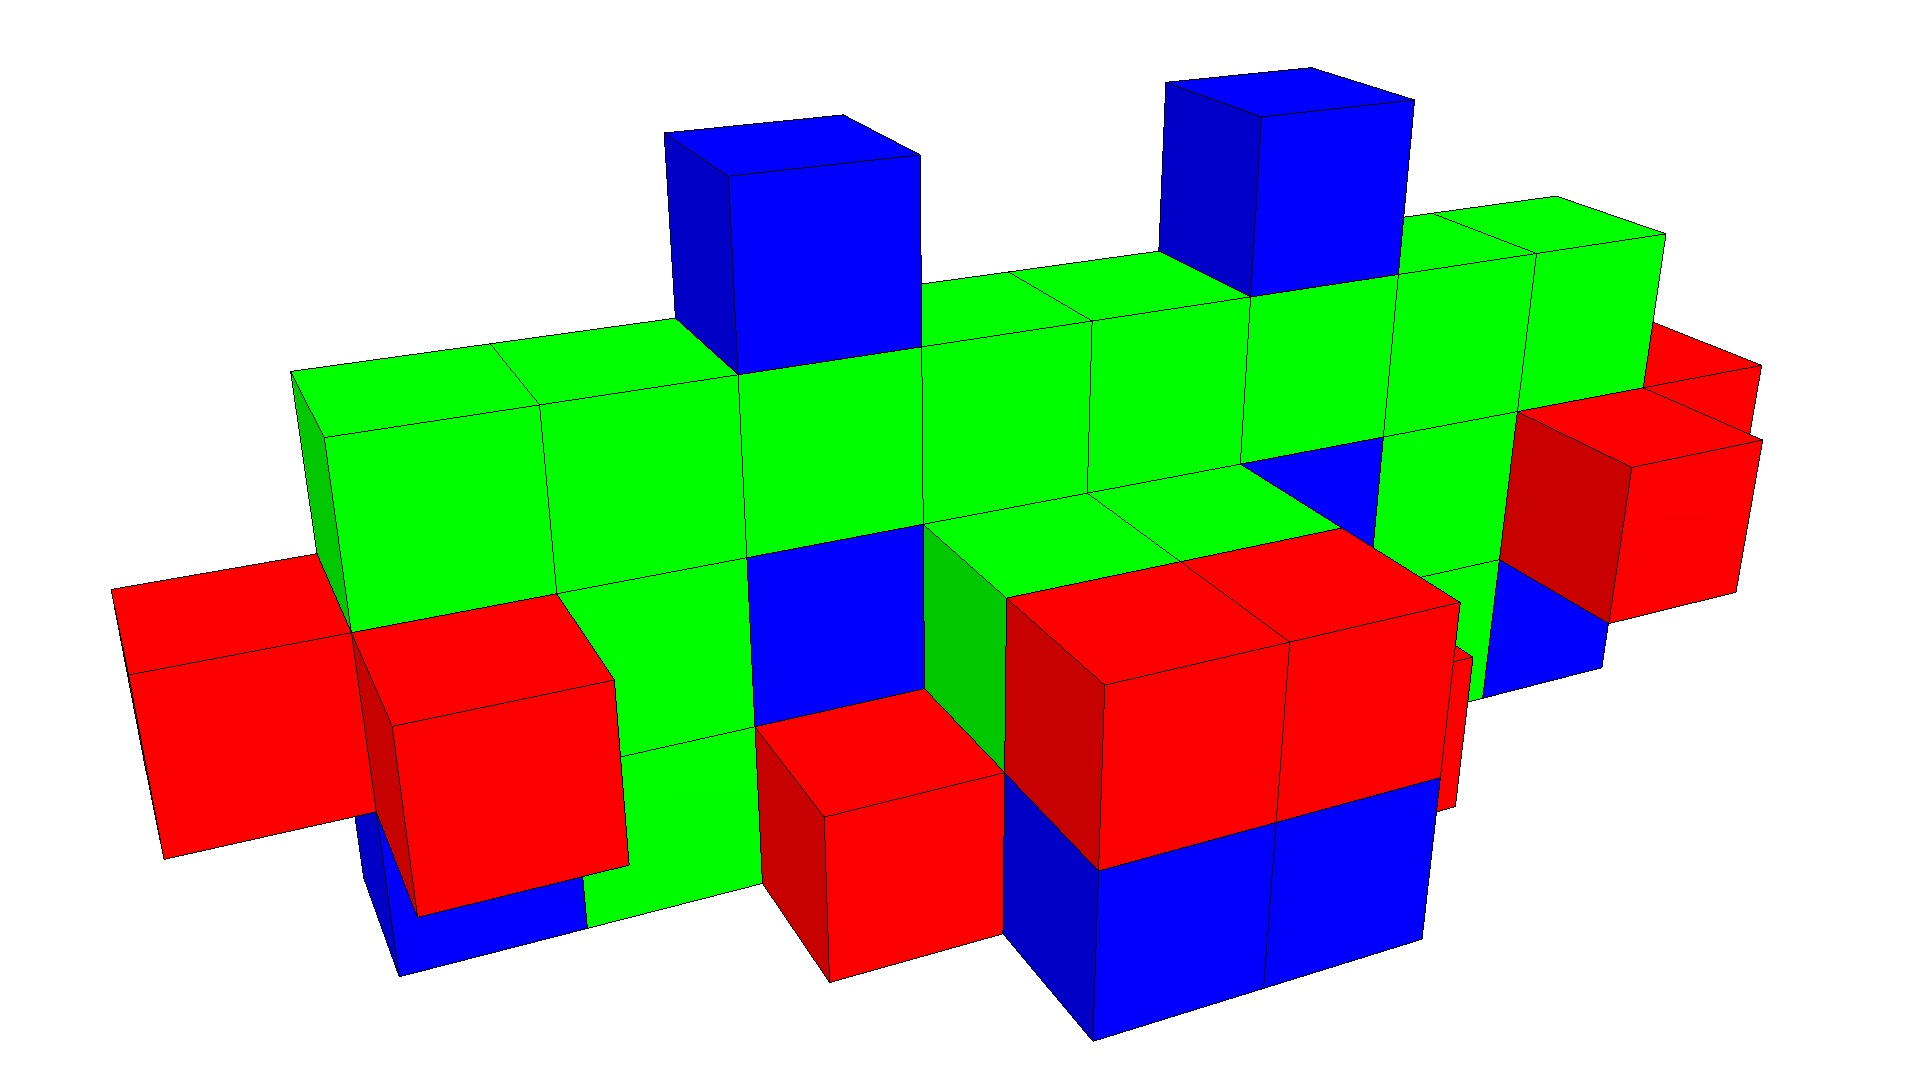
\includegraphics[height=0.15\textwidth]{../Figures/Robots/rg1.jpg}
\caption{Generative encoding creates more natural morphologies even in random schemes.}
\label{fig:randomResultsRobots}
\end{figure}


The indirect random morphology generation follows a different method of assigning materials to voxels. This methods holds two probabilities, the one refers to the probability of adding a new voxel in the already made structure, the next one denotes the probability of the new inserted material will be the same as its connection's material. First, a voxel of random material is inserted in a random coordinate into the lattice. If a new voxel is to be added a connection (voxel) is chosen from the already inserted ones. The side of the connection is chosen randomly as well, although the material itself is most of the times the same as it connected voxel's material. In this generative process there is also the possibility of creating structures in half of the lattice space, and then mirror the soft structures in both halves.

Considering these two methods, the difference between direct and indirect coding is becoming easier interpreted. In the direct process, a probability determines the presence and the material of every voxel in the lattice. On the other hand, in the generative method a set of rules and probabilities define the structure that is going to be produced into the available space.

Figure~\ref{fig:randomResultsRobots}, illustrates not only the actual performance (top-$1000$ soft-robots from $30000$ total runs for each method) of the previously described method but also one of the best performing robots of each method. Both generative methods outperform the direct one, mostly because there is no structure in the created creatures, another one reason is that since there are no rules in the construction of the random structures resulting in morphologies with huge number of voxels, something that makes them difficult to locomote. On the other hand, generative random methods create more compact structures which can move easier due to their size and some of their geometrical features. For the mirrored approach even though the average performance is slightly worse than the plain method it actually performs way better in some distinct cases. Inserting some geometrical properties like properties resulted in getting more successful locomotive structures. 

\section{Direct-Encoded Evolutionary Soft-Robots}

\begin{figure}
\centering
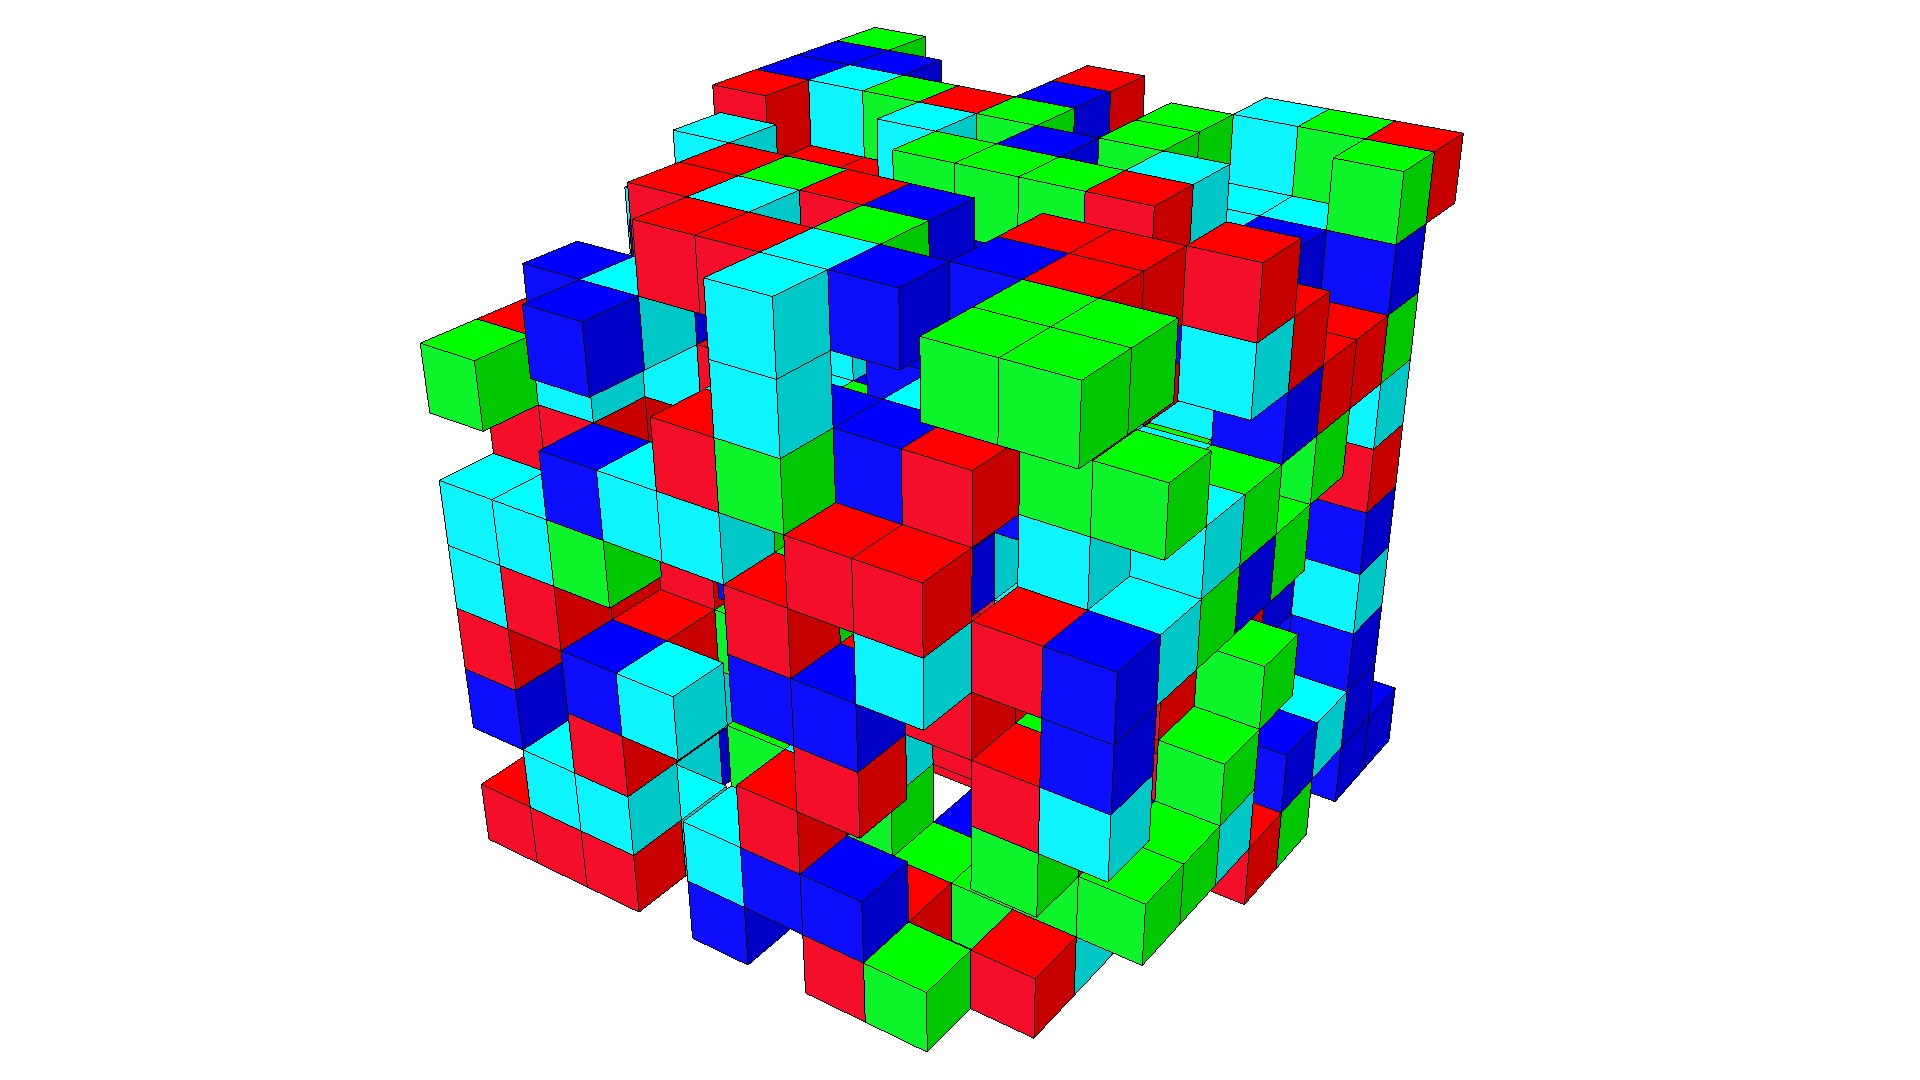
\includegraphics[height=0.2\textheight]{../Figures/Robots/direct.jpg}
\caption{Direct encoding cannot capture the geometrical properties of some problems.}
\label{fig:directRobot}
\end{figure}

In the previous section, indirect and direct random morphology methods were implemented and tested, failing to produce any decent locomotion gaits for the soft structures. Considering how vast is the solution space, random approaches are doomed to fail in a definite number of tries. 

Hence, a more sophisticated method is tested here. Direct encoding genomes coupled with a simple genetic algorithm is a successful approach in evolving robot controllers. As it was previously stated in ch.~\ref{Background}, mutations and crossovers of real value streams, search the space effectively succeeding in difficult optimization problems. GAlib C++ library \cite{wall1996galib}, used for the implementation of this method.

\paragraph*{Representation of the genotype}~\\
As in every direct encoding scheme, genotype can be represented by a stream of bits, which length is equal with the number of the dimensions of the problem. In this case, using 4 materials but also trying to encode the presence of each voxel in the lattice as another dimension of the problem. Analytically, its length can be represented by a stream of length equal with the number of voxels in the lattice times the materials used plus one denoting the presence, descibed by the following equation:
\begin{equation}
\label{lengthDirect}
| Genome | = (l_x \times l_y \times l_z ) \times (1 + |p|)
\end{equation}
, where $l_x, l_y, l_z$ are the dimensions of the lattice space, and $p$ is the palette of materials.
\begin{equation*}
Genome = \underbrace{01010\ldots011011}_\text{Presence}\ \    \underbrace{10101\ldots110011}_{Material_1} \   \ldots\  \underbrace{00011\ldots111110}_{Material_n}
\end{equation*}
The above stream of bit illustrates how a soft-structure in VoxCad environment can be represented. Each of the values of the stream is represented by a value between zero and one, which represented 
in the algorithm by a stream of bits. \emph{Alleles} are continuous numbers in that case, alleles is the definition of each value of the chromosome, which are not shown above due to visualization simplicity. The mapping from the genotype level to the phenotype is straightforward in this case, the first stream of values is used to determine the presence or not for a voxel, while in case of a presence the other $n$ streams are used and the maximum value in specific positions of the streams determine the material is going to be used.

Considering the representation of the genome, as well as the geometrical nature of the problem it self, it is valid to say that we do not expect that direct encoding will capture this major property of the problem (Fig.~\ref{fig:directRobot}).

\section{Generative-Encoded Evolutionary Soft-Robots}

Direct encoding schemes lack the regularity of their designs in the phenotype level leading in morphologies that cannot produce any coordinated locomotion behaviors. Generative-Indirect encoding (CPPN) as it previously explained in detail, serves this function. Producing regularities in the phenotype space, and capturing geometrical properties of the optimization problem, it is expected to produce fine locomotion strategies and morphologies of the soft structures~\cite{cheney2013unshackling}.

\begin{figure}
\centering
\includegraphics[height=0.2\textheight]{../Figures/Misc/cppnSoftBot2.eps}
\caption{Each genotype is queried for every coordinate inside the lattice, its outputs determine the presence of a voxel and the type of its material.}
\label{fig:cppnDiagram}
\end{figure}


Compositional pattern producing networks are built up by a set of canonical functions which force the outputs of the network to produce repetitive, symmetrical and geometrically interesting patterns. Since, CPPNs must queried for every coordinate of the lattice space, the input nodes of the CPPN were assigned to x,y,z normalized coordinates, following~\cite{cheney2013unshackling}. It should be pointed out here that more inputs could be added to the CPP-network, such as the the distance from the center point of the Cartesian space (simulation lattice) as described in~\cite{stanley2007compositional}, which naturally adds more bias towards symmetrical structures, than CPPNs already do. What is more, creating perfectly symmetrical structures is not much of an interest to show, since CPPNs during evolution, since as shown later in this thesis, it can evolve symmetrical shapes without this symmetrical information input node. Figure~\ref{fig:cppnDiagram}, illustrates the topology of a random CPPN network with the input and output nodes described above. Every connection node between input and output nodes is called the network's \emph{topology} which can be variant and be evolved alongside the weights of the connections in an evolutionary method like NEAT. The shaded part of the network is the part that it is actually the one that describes the genotype and how the phenotype will be structured, while differently colored nodes denote different functions used in them.
Once again, the presence or not of a voxel in a lattice coordinate is determined by a single output of the CPPN called $p$ and the selection of the material out of the palette is again determined by $n$ outputs, the node will the maximum value in the output will determine which of the $n$ materials will be used.


\subsection{How CPPNs can be evolved?}
The evolution of these indirect representations of the phenotypes can be evolved with any method able to evolve artificial neural networks, since they are identical with CPPNs. CPPN-NEAT (first described in Ch.~\ref{Background}), is a method of evolving CPPNs with NEAT evolutionary method, was chosen to evolve those networks as it has proven successful in previous work in the same setting~\cite{cheney2013unshackling}. HyperNEAT \texttt{v4.0 C++} by J. Gauci code (url: \url{https://github.com/MisterTea/HyperNEAT}) was used for the experiments. Algorithm~\ref{evolutionPseudocode}, presents the pseudocode for the evolution under CPPN-NEAT method. In addition, a brief explanation of each function used in the algorithm follows:


\begin{algorithm}[t!]
\caption{CPPN-NEAT evolution}
\label{evolutionPseudocode}
\begin{algorithmic}[1]
\STATE $\mathtt{population} = \varnothing$
\STATE $\mathtt{species} = \varnothing$
\STATE $\mathtt{generation}[0] = \mathbf{initial\_population}()$
\FOR{ $i = 0\   \text{to}\  \mathtt{max\_generation}$}
\STATE $\mathtt{species} = \mathtt{species} \cup \mathbf{speciation}(\mathtt{generation}[i])$
\STATE $\mathbf{evaluation}(\mathtt{generation}[i])$
\STATE $\mathbf{adjust\_fitness}(\mathtt{generation}[i], \mathtt{species})$
\STATE $\mathbf{selection}(\mathtt{generation}[i], \mathtt{species})$
\STATE $\mathtt{generation}[i+1] = \mathbf{reproduction}(\mathtt{generation}[i])$
\STATE $\mathtt{population} = \mathtt{population} \cup \mathtt{generation}[i+1]$
\ENDFOR
\end{algorithmic}
\end{algorithm}

\clearpage % to fit in a page
\begin{framed}
\begin{description}
\item[Initial population]{Before the evolution starts, an initial population must be produced, random genomes (CPPNs) fill up the population.}
\item[Speciation]{ ,takes place and split the population in different species or adds individuals to already existing species in respect to their network's topologies. However, all firstly introduced genomes belong to the same species, due to the identical topology of their CPPNs.}
\item[Evaluation] Once the population is filled with new individuals, these have to be evaluated. Simulation is take place for each of the individuals of the population, whereas each one of them is awarded with a fitness value.
\item[Fitness adjustment]{After all individual are evaluated, each species is assigned a value which is the sum of the fitness values of the individuals belonging to the species divided by the number of the individuals. The way it is been decided how many individuals each of the species will breed is directly determined by the average fitness of each species.}
\item[Selection]{As soon as the number of new individual each species is determined, only the top $20\%$ of the species population will reproduce, the rest population will ``die''.}
\item[Reproduction]{There are three ways, for the selected individual inside each species to reproduce. The first is called \emph{elitism}, meaning that the best of each species will copy itself in the next generation. The next two are \emph{mutation}, which changes the genome of one individual slightly and creates a new genome for the next generation, and \emph{crossover} which is the most natural operator and it uses mixes two parent individuals to create a new genome.}
\end{description}
\end{framed}






\subsection{Novelty search}
Novelty search as first presented in Ch.~\ref{Background}, requires small changes in an evolutionary algorithm. Fitness is replaced by a novelty metric which determines how different is a phenotype's behavior in respect to novel behaviors found before. Sparsity (eq.~\ref{sparsenessEquation}), is used to dermine this measure, whereas every individual is compared not only with the previous novel behaviors but also with the current generation individual behaviors. 



\begin{algorithm}[t!]
\caption{CPPN-NEAT with novelty search}
\label{noveltyPseudocode}
\begin{algorithmic}[1]
\STATE $\mathtt{population} = \varnothing$
\STATE $\mathtt{novel\_inds} = \varnothing$
\STATE $\mathtt{species} = \varnothing$
\STATE $\mathtt{generation}[0] = \mathbf{initial\_population}()$
\FOR{ $i = 0\   \text{to}\  \mathtt{max\_generation}$}
\STATE $\mathtt{species} = \mathtt{species} \cup \mathbf{speciation}(\mathtt{generation}[i])$
\STATE $\mathbf{evaluation}(\mathtt{generation}[i])$
\FORALL {$\mathtt{ind} \in \mathtt{generation}[i]$}
\STATE $\mathtt{novelty} = \mathbf{sparsity}(\mathtt{ind}, (\mathtt{generation}[i] - \mathtt{ind}) \cup \mathtt{novel\_inds})$
\IF {$(\mathtt{novelty} \geq \mathtt{novelty\_{threshold}}\ ||\ \mathtt{novel\_inds} == \varnothing)$}
\STATE $\mathtt{novel\_inds} = \mathtt{novel\_inds} \cup \mathtt{ind}$
\ENDIF
\ENDFOR
\STATE $\mathbf{adjust\_novelty}(\mathtt{generation}[i], \mathtt{species})$
\STATE $\mathbf{selection}(\mathtt{generation}[i], \mathtt{species})$
\STATE $\mathtt{generation}[i+1] = \mathbf{reproduction}(\mathtt{generation}[i])$
\STATE $\mathtt{population} = \mathtt{population} \cup \mathtt{generation}[i+1]$
\ENDFOR
\end{algorithmic}
\end{algorithm}


The algorithmic adjustments are presented in Algorithm~\ref{noveltyPseudocode}, where the pseudocode of novelty search is presented. Instead of just returning a fitness value, function \textbf{evaluation} has as an output the behavior of the individual evaluated, as well as its fitness for comparing purposes. Function \textbf{sparsity}, computes the sparseness of a specific individual's behavior in the behavioral space, calculating the mean distance from the $k$-closest behaviors. Following the evaluation of each individual and the returned point in the behavior space, if the novelty metric is larger than a threshold, this individual will enter the novelty individuals' set. The fitness adjustment of the previous code example is becoming novelty adjustment following the same functionality, selection and reproduction methods are working in the same fashion, whereas they are comparing the novelty of the individual in the place of their fitness.


\subsubsection{Behavior in novelty search}

\begin{table}
\centering
\caption{Behaviors used for novelty metric computation, to evolve morphologies for the soft-robots.}
\label{Behaviors}
    \begin{tabular}{lrcc p{4cm}}
    \toprule
    \textbf{Behavior} &
    \textbf{Sampling} &
    \textbf{DFT} &
    \textbf{Example} &
    \textbf{Description} \\
    \midrule
    \Vcentre{3D-trajectory}    &
    \Vcentre{1 KHz}     &                       &
    \Vcentre{\includegraphics[scale=0.19]{../Figures/Behaviors/3d.pdf}} &
    \vspace{-.85cm}Set of three dimensional sampled points of the robot's center of mass during simulation.  \\
    \Vcentre{2D-trajectory}   &
    \Vcentre{1 KHz}     &                     &
    \Vcentre{\includegraphics[scale=0.18]{../Figures/Behaviors/2d.pdf}} &
    \vspace{-.85cm}Set of two dimensional ground projection sampled points of the robot's center of mass during simulation.      \\
    \Vcentre{Pace}                 &
    \Vcentre{1 KHz}     &                     &
    \Vcentre{\includegraphics[scale=0.18]{../Figures/Behaviors/pace.pdf}} &
    \vspace{-.85cm}Set of robot's pace sampled values.    \\
    \Vcentre{DFT-Pace}             &
    \Vcentre{100 KHz}   &
    \Vcentre{\checkmark}                &
    \Vcentre{\includegraphics[scale=0.18]{../Figures/Behaviors/pacedft.pdf}} &
    \vspace{-.9cm}Set of the robot's pace sampled values transformed into the frequency space.    \\
    \Vcentre{VTG}                  &
    \Vcentre{1 KHz}     &                     &
    \Vcentre{\includegraphics[scale=0.18]{../Figures/Behaviors/vtg.pdf}} &
    \vspace{-.85cm}  Voxels touching the ground in each sampling time.  \\
    \Vcentre{DFT-VTG}              &
    \Vcentre{100 KHz}   &
    \Vcentre{\checkmark}              &
    \Vcentre{\includegraphics[scale=0.18]{../Figures/Behaviors/vtgdft.pdf}} &
    \vspace{-.85cm} Voxels touching the ground transformed into the frequency space.   \\
    \Vcentre{Pressure}             &
    \Vcentre{1 KHz}     &                     &
    \Vcentre{\includegraphics[scale=0.18]{../Figures/Behaviors/pr.pdf}} &
    \vspace{-.85cm}Maximum pressure among the connected voxels.  \\
    \Vcentre{DFT-Pressure}         &
    \Vcentre{100 KHz}   &
    \Vcentre{\checkmark}                &
    \Vcentre{\includegraphics[scale=0.18]{../Figures/Behaviors/prdft.pdf}} &
    \vspace{-.85cm}Maximum pressure among the connections transformed into the frequency space.    \\
    \Vcentre{KE}                   &
    \Vcentre{1 KHz}     &                     &
    \Vcentre{\includegraphics[scale=0.18]{../Figures/Behaviors/ke.pdf}} &
    \vspace{-.85cm}Maximum kinetic energy of voxels.    \\
    \Vcentre{DFT-KE}               &
    \Vcentre{100 KHz}   &
    \Vcentre{\checkmark}                &
    \Vcentre{\includegraphics[scale=0.18]{../Figures/Behaviors/kedft.pdf}}  &
    \vspace{-.85cm}Maximum kinetic energy of voxels transformed into the frequency space.    \\
    \bottomrule
    \end{tabular}
\end{table}

In the interest of novelty to be defined, behaviors should be defined that make sense in our problem setting. Trying to optimize locomotion strategies of soft-robots under variant environment in fitness-based methods, a good measure is the displacement under a limited time-span. On the contrary, novelty search is in a need of a behavior metric that encodes these fitness attributes inside. Novelty search forces the evolution to try new behaviors, if the objective cannot be encoded in the behavior, the search then novelty search will become random. As an example, the number of voxels a soft robot has is not a well-founded behavior metric, since the search will reward new structures with different number of voxels from previous ones, there will be no exploration in a metric that affects the actual target of the evolution which is to produce and evolve good locomotion strategies. Table~\ref{Behaviors}, presents all behaviors used for novelty metric computation, with the sampling rates of the recorded values during the simulation and a description. 

All these behaviors designed having in mind that enough information about the locomotion success must be encoded into the behavior's recorded signal. Trajectories (2D and 3D), incorporate all the needed information, such as speed, displacement, locomotion strategy. To avert from same trajectories in all possible directions, trajectories are normalized, meaning that their starting coordinate in both cases (2D and 3D) is always the start of the axes, and their all coordinates of the trajectory are rotated so their center of mass coordinate is normalized to meet a certain angle. Computing the difference of two trajectories, the Euclidean distances of all coordinates of the one trajectory are computer in respect to coordinates at the same sampling time.

Pace is also a very informative behavior metric as it directly measures the speed of the robot. Voxels touching the ground can also produce information about the locomotion strategy but not enough about the actual performance speed-wise. Hopping robots that move fast can have same behaviors with hopping robots with zero speed. Maximum pressure among the voxels' connection is one more behavior metric, pressure is expected to become higher as structures move faster and interactions with the ground eventually being harder. Finally, maximum kinetic energy is a different behavior that straightly determines the displacement of the voxels in the structure. For all behaviors but trajectories, the Fourier profile of their signal can also be used as a behavior signature of the individuals, which can also eliminate shifts of signals in time-axis. To compute the difference of over two signals a straightforward method is chosen. Subtracting the one signal from the other taking the absolute differences and sum them up to compute one signle value that describes how variant the two signals are. Furthermore, for the Fourier transformations of these signals, the first twenty coefficients are compared, the absolute sum difference again determines the difference.
% Chapter 5

\chapter{Results} % Main chapter title

\label{Results} % For referencing the chapter elsewhere, use \ref{Chapter1} 

\lhead{Chapter 5. \emph{Results}} % This is for the header on each page - perhaps a shortened title

Following the comprehensive analysis of the evolutionary methods used in the experiments in the previous chapter, in this chapter the performance of these methods is compared and analyzed. Pure novelty search is compared in respect to the fitness measure used in the simulations (displacement of soft-robots in body-lengths), against fitness search. Questions, as far as what happens in the average fitness and the champion fitness of each generation within novelty search, answered in the following sections. Additionally both search methods are compared in respect to the number of novel behavior they generate during an evolution experimental run. The effect the behavior metric selection has in novelty search is also considered, as well as, the number of closest behaviors in sparsity equation plays also an important role in the evolution towards diversity of behaviors. Selection techniques such as competition within species are also used in both search methods, to determine the effects they have in the performance towards the specific goal it has been set. A new method is proposed for incorporating fitness information into novelty search without unbalancing the search for novelty and its properties. Last, the performance of both methods are now investigated within variant gravity levels, in order to show that gravity conditions do not have an effect towards a specific search method, as well as to examine different evolved locomotion strategies under different gravity conditions.

As in~\cite{cheney2013unshackling} and for comparison purposes, the population of each generation used is $30$, and the number of generations of the evolution is $1000$. For more details about the evolutionary algorithm and simulation settings used, see appendix~\ref{AppendixA}. Due to computationally expensive simulations, lattice sizes less than $10^3$ have been used as well, more specifically experiments have been done under $5^3, 7^3, 10^3$ lattice space.

\begin{figure}[ht!]
\centering
\includegraphics[width=1.0\textwidth]{../Figures/Results/indRunnAvgSize7Fitness.pdf}
\caption{Best so far fitness, $10$ individual runs for fitness based search (settings~\ref{Settings3}).}
\label{fig:indRunsAvgSize10Fitness}
\end{figure}
~
\begin{figure}[ht!]
\centering
\includegraphics[width=1.0\textwidth]{../Figures/Results/indRunnAvgSize7Novelty.pdf}
\caption{Best so far fitness, $10$ individual runs for novelty search (settings~\ref{Settings3}).}
\label{fig:indRunnAvgSize10Novelty}
\end{figure}


\section{Into The Performance of Novelty Search}

Before compare novelty search to fitness based search, it is of interest to show how individually perform under the same simulation settings.

Figure~\ref{fig:indRunsAvgSize10Fitness} shows $10$ independent runs for fitness based search. Following the objective function's gradient fitness based evolution does small step towards better and more optimized individuals from generation to generation. What is more, fitness based evolution often sticks into specific morphologies which then tries to optimize leading the evolution to stop at that local maximum.

Figure~\ref{fig:indRunnAvgSize10Novelty} shows $10$ independent runs for novelty  search. In comparison with the same figure for fitness based search (fig.~\ref{fig:indRunsAvgSize10Fitness} we can see a clear difference. Evolving for novelty means that within the evolution only a novel behavior is rewarded instead of a good behavior or a behavior that leads to the optimization of the objective function. Big steps in the fitness value on all independent runs can be observed which can lead us to a conclusion that fit individuals in respect to the objective function for which novelty search has no information within the evolution process, are results of new novel behaviors. 

One more thing worth noticing, is that observing only big steps in the fitness, we can derive that there is no optimization of morphologies within novelty search. Initially, novel individuals are highly rewarded, these individuals can be very good in respect to the fitness or not, the algorithm does not consider the ``goodness'' of these individuals, and does not have any information regarding this either. On the next generation, mutations, crossovers, and copies of these novel individuals are not going to be highly variant in respect to their chromosome from their ancestors, resulting to similar behaviors, which are  not going to be remarkably rewarded in respect to their novelty value. Thus, highly novel individuals are producing less novel children, meaning that these children, even though their fitness is high and can be optimized further, will not have the chance to reproduce in the next generations and be improved eventually, as in fitness based evolution.

\begin{figure}[t!]
\centering
\includegraphics[width=1.0\textwidth]{../Figures/Results/FitNovRandomDirectSize5.pdf}
\caption{Comparison of simple genetic algorithm (direct encoding) against \emph{random} - \emph{fitness} - \emph{novelty} search with generative encoding. Best so far fitness averaged over $10$ runs (settings~\ref{Settings1}).}
\label{fig:FitNovRandomDirectSize5}
\end{figure}

\begin{figure}[t!]
\centering
\includegraphics[width=1.0\textwidth]{../Figures/Results/FitvsNovVsDirSize10.pdf}
\caption{Comparison of simple genetic algorithm (direct encoding) against \emph{fitness} - \emph{novelty} search with generative encoding. Best so far fitness averaged over $10$ runs (settings~\ref{Settings2}).}
\label{fig:FitvsNovVsDirSize10}
\end{figure}

To extensively compare the performance achieved by novelty search method the same experiment held under two different simulation settings (for sizes $5^3$ ,$10^3$), set side by side with fitness search, random search, and finally a simple genetic algorithm. Notice, that the first three methods are referring to a generative encoding (CPPNs) evolved by Hypercube NEAT evolutionary algorithm and using selection in respect to fitness, novelty and finally random selection, while the latter uses a direct encoding scheme driven by fitness. 

Novelty search to perform the novelty metric computation, makes use of the two dimensional trajectories, which are all normalized so that their centre of mass of the trajectories coordinates meet a specific angle, as well as their starting coordinate is always located in the beginning of both axes. Fitness-based search objective function is the displacement of the soft-robot's center of mass from its initial position in body-lengths. Random evolution with Hypercube NEAT achieved using random selected individuals to breed. For direct encoding, the method used is has been explained in Chapter~\ref{Method}. 

Figure~\ref{fig:FitNovRandomDirectSize5}, presents the results for the small sized structures ($5^3$). Notice, the difference between novelty search and fitness-based method, novelty evolves structures that are superior than any other method does in these settings. At this point, it should be mentioned that in such a small structures locomotion patterns cannot be evolved due to the stability issues of the simulator, and due to the fact that lightweight structures can be bouncy, leading to ball shaped structures capable of achieving large displacement from their initial positions. That being said, we still have to deal with an optimization problem, where local optima and global ones can be found as the number of the possible solutions in this setting, using 4 materials, is $\sim 2,3 \times 10^{87}$. Using the trajectories of the soft-robots, novelty search visits optimal solutions that none of the other methods does because of local optima (fitness-based search), due to encoding limitations (direct encoding), or random search which selects random individuals to reproduce without caring about their performance, and with no backtracking (there is no guarantee that random search will visit new behaviors). The simple genetic algorithm approach which uses a direct encoding to represent the structure of the soft-robots performs better than using random selection within an indirect encoding evolution pointing out that symmetry does not provide any merits to the evolution for these sizes soft-body robots.

Moving to a larger lattice space size we expect indirect encoding to prove its advantages over the direct encoding scheme~\cite{cheney2013unshackling,stanley2007compositional}. Furthermore, novelty search now has a more difficult task as the space of possible behaviors (2d-trajectories) becomes larger as more complicated morphologies can now be produced (morphology space for $10^3$ lattice space: $9.3 \times 10^{698}$). To try to solve all these research question the same experiment held under a lattice of size $10^3$. 

Figure~\ref{fig:FitvsNovVsDirSize10}, presents the results of the same four different methods in this setting. Results reassure that novelty search achieves higher fitness on average against fitness-based search. Nevertheless, there is no tremendous difference as in the previous experiment, discovering that at their individual runs they both achieve to evolve the soft-robot structure with the highest fitness found in all experiments ($\sim 14$ Body lengths). Novelty search seems more constant in evolving individuals with high fitness in all runs, on the other hand most of individual runs of fitness search trapped in a low fitness local optimum structure, trying to optimize the specific individual genotype without trying to explore more the fitness landscape like novelty did successfully. Once again, random evolution with Hypercube NEAT is producing decent structures for soft-robots but cannot climb the hill of fitness, going in every direction, at the same time making more and more complex network topologies for CPPNs. Earlier in this thesis, in chapter~\ref{Background}, generative encoding advantages over direct explained in detail, here their superiority can evidently be observed. Direct encoding performance when a larger lattice for the simulation used, was radically decreased, mostly because structure and morphology regularity is a necessity for the soft-robots in order to perform decently in these sizes, something that direct encoding cannot capture failing to produce anything useful.






\begin{figure}[t!]
\centering
\includegraphics[width=1.0\textwidth]{../Figures/Results/AvgGenerChampNoveltyFitnessSize7.pdf}
\caption{Fitness of the generation's champion (best individual) for \emph{fitness} - \emph{novelty} search averaged over $10$ runs (settings~\ref{Settings3}).}
\label{fig:AvgGenerChampNoveltyFitnessSize7}
\end{figure}

Another aspect of the evolution should be inspected is how the population of each generation is affected in respect to the best individual per generation, especially thinking about the these generation champions is the ones that result in the increased of novelty search when compared with fitness based search. In figure~\ref{fig:AvgGenerChampNoveltyFitnessSize7}, the champions' fitness (Best fitness found within each generation) of each generation is plotted averaged over $10$ runs. Recall, that novelty search does not have any information about fitness of individuals. In fitness based search there is a clear trend that champions of each generation are getting better through the evolution resulting to an approximately monotonically increasing function. On the other hand, generations' champions in novelty search apart from the early improvement which is mainly caused by the generative encoding, follow a random pattern. What it is interesting here to see is that even though that the solutions novelty search gives, in this settings (lattice size: $7^3$), are clearly better than the ones evolved by fitness based search, on average the champions during novelty search evolution are worse. Hence, individuals that resulting in the increased performance of novelty search clearly lie on the tail of the fitness distribution on each generation.


\begin{figure}[t!]
\centering
\includegraphics[width=1.0\textwidth]{../Figures/Results/ViolinPlotsAvgGenFitSize7.pdf}
\caption{Distributions of average population fitness per generation over 10 runs for \emph{fitness}(Blue) - \emph{novelty} (Green) search with generative encoding (settings~\ref{Settings3}).}
\label{fig:ViolinPlotsAvgGenFitSize7}
\end{figure}

In the same fashion, the average population fitness seems also affected by the different optimization methods. Figure~\ref{fig:ViolinPlotsAvgGenFitSize7} illustrates the distribution of population's average fitness over $10$ independent runs for \emph{novelty}-\emph{fitness} based search every $100$ generations. The resulted distributions which are shown in violin-like shapes clearly show that the average generation's fitness remains stable through the whole evolution ($1000$ generations) for both methods. What is more, the generation's average fitness is significantly lower for \emph{novelty} search, meaning that when the evolution is being carried towards novel behaviors there is no such guarantee that assumes novel new founds in the behavioral space will also be \emph{fit}. 

What we see in the last two figures, evidently shows that even though novelty search achieves in finding more ``fit'' solutions than fitness based search in the specific problem domain, the average fitness of both generation champions and population remain lower than in fitness based search.

\begin{figure}[t!]
\centering
\includegraphics[width=1.0\textwidth]{../Figures/Results/novelIndividualsFitNovComp.pdf}
\caption{Number of novel behaviors found up to generation number, averaged over 10 runs. The novelty measure is computed as the average distance from the $10$-nearest behaviors for \emph{fitness} - \emph{novelty} search with generative encoding (settings~\ref{Settings3}).}
\label{fig:novelIndividualsFitNovComp}
\end{figure}

Until this point, the performance of both fitness and novelty search methods have been compared in the same objective metric such as the displacement of the produced soft body robots. The former method method tries to optimize genomes in respect to the specific objective function, while the latter moves its interest into creating diversity of the population in the behavioral space. As shown before, the novelty search achieves to create novel individuals which are not only novel in respect to how different behaviors they have from the rest of the population they exist into, but also they achieve higher average fitness than those they are optimized towards that objective. Inverting the objective function now such as our goal is to generate a wide variety of behaviors, in this case, two dimensional trajectories, we expect that a much larger set of novel behaviors will be created by novelty search. Figure~\ref{fig:novelIndividualsFitNovComp}, presents the number of unique behaviors the two evolutionary methods found, averaged over $10$ runs. The resulted graph shows that comparing these two methods is pointless as \emph{novelty} search can force the evolution towards spaces in the behavioral space that have not visited, finding more novel individuals, which does not happen in the fitness search. Surprisingly, \emph{novelty} achieves better performance than \emph{fitness} search in both objectives set so far, creating fit, and at the same time diverse solutions.

\begin{figure}[t!]
\centering
\includegraphics[width=0.49\textwidth]{../Figures/Behaviors/behaviorsNovelty.pdf}\	
\includegraphics[width=0.49\textwidth]{../Figures/Behaviors/behaviorsFitness.pdf}
\caption{Novelty search creates a vast amount of behaviors achieving in this way to find fit individuals, and avoid local optima of the solution space. (settings~\ref{Settings3})}
\label{fig:behaviorSpaceDiversity}
\end{figure}

To visualize the difference in the behavior space of the two methods, figure~\ref{fig:behaviorSpaceDiversity}, illustrates all the stored found novel behaviors (two dimensional trajectories) found in one evolution run of novelty and fitness search using the same novel measure to determine the novelty of a behavior.

\subsection{How Behavior Selection Affects \emph{Novelty}-Search}

A good behavior metric should include information about the objective function. In case of locomotion gait of soft robots a trajectory can be highly informative as far as the displacement of the robot's body is concerned. Two robot bodies which travelled the same distance into an equal time horizon, should have the same fitness if displacement only is measured, nevertheless, the locomotion strategy, is something that can only affect the actual behavior metric and not the objective function. Forcing the evolution to seek for the different in the behavior space results in finding $>10 \times$ more novel behaviors than \emph{fitness} search (depending on the threshold and the behavior metric), which  indirectly implies that high fitness individuals will be found. How the behavior metric affects the performance of the evolution is discussed in detail in the next section.

\begin{figure}
\centering
\includegraphics[width=1.0\textwidth]{../Figures/Results/FitNovSize5Pen2.pdf}
\caption[]{Best so far fitness averaged over $10$ runs, penalizing actuated materials\footnotemark for \emph{fitness} - \emph{novelty} search with generative encoding (settings~\ref{Settings1}).}
\label{fig:FitNovSize5Pen2}
\end{figure}

\footnotetext{Actuated materials penalize fitness: \[f = (1 - (n_{actuated} / n_{total})^{1.5}) \times disp \], where $n_{actuated}$, is the number of actuated voxels, $n_{total}$ total number of voxels and $disp$ the displacement of the softbot's center of mass.}


The importance of selecting a good behavior metric is important in order for novelty search to explore the behavior space to a great extent. For example searching for fast robots while you exploring the behavior space of their trajectories is a wise decision considering that all information needed to determine the fitness (speed) is incorporated inside the behavior (trajectories) assuming static sampling rate of the trajectories. In this experiment to investigate what is the result of the novelty-search evolution when no information is provided by the behavior, the behavior selected has not enough information about the actual individual fitness. The two dimensional projection of the trajectories in $x,y$-axis are again selected, while instead of evaluating the fitness in displacement, this displacement is penalized by the number of actuated voxels are inside the structure of the soft robot. Figure~\ref{fig:FitNovSize5Pen2}, illustrates the best so far fitness for both novelty and fitness search averaged on $10$ independent runs. Comparing the results with figure~\ref{fig:FitNovRandomDirectSize5}, one can notice how novelty search performs poorly in this setting. Considering that the same method outperforms traditional fitness-search evolution when the whole information of the fitness function is contained in the behavior. Trying to find novel trajectories in the first case proved successful in respect to the final displacement of the individual, from the other hand trying to maximize the distance and in the same time use few actuated voxels proved crucial for the final outcome. If the number of actuated voxels had been included in some way into the behavior, novelty-search would have been more explorative towards this direction as well.


\begin{figure}
\centering
\includegraphics[width=1.0\textwidth]{../Figures/Results/KnnExperimentSize5.pdf}
\caption{Best so far fitness averaged over $10$ runs (settings~\ref{Settings1}), for different $k$ to sparsity computation of the behavior.}
\label{fig:KnnExperimentSize5}
\end{figure}

\begin{figure}
\centering
\includegraphics[width=1.0\textwidth]{../Figures/Results/BehaviorsPerformance.pdf}
\caption{Right, comparison of the evolution's best fitness result from $10$-runs under different behavioral metrics for \emph{novelty} search. \emph{Fitness} search is also evaluated under the same settings. (settings~\ref{Settings3}).}
\label{fig:BehaviorsPerformance}
\end{figure}

Sparsity (eq.~\ref{sparsenessEquation}) is the measure that defines if a newly found behavior is novel enough to enter the set of novel behaviors. Figure~\ref{fig:KnnExperimentSize5} presents the resulted best so far fitness given different values for $k \in \lbrace 1, 2, 5, 10, 20 \rbrace$. In principle $k$ can define how tolerate the algorithm can be with new behaviors. It is not certain that a specific value for $k$ should give the highest performance in fitness and it depends almost completely by the application. The only implication in choosing value for $k$ is that choosing large values should yield in a more detailed exploration in the behavior space, in the contrary using small values final set of behaviors will be denser in the behavior space. In the specific figure and experiment $k=10$ was the setting that led to the best performance.


Choosing the appropriate metric to describe a phenotype into the behavior space is crucial in the performance of novelty search. Figure~\ref{fig:BehaviorsPerformance} illustrates the experimental results under different behavior metrics, alongside the performance of pure \emph{fitness} based optimization. A set of $10$ different behavior types was used including the three dimensional trajectories of the soft robots (3D-Traj), the two dimensional projection on $x,y$-axes of the previous behavior (2D-Traj), the pace sampled every $0.001$ sec. (Pace), the discrete Fourier transformation of the same signal which was sampled every $0.00001$ sec. (DFT-Pace), the voxels touching the ground on each time-step (VTG, DFT-VTG), the maximum pressure per time-step (Pr, DFT-Pr), and the kinetic energy of the whole structure (KE, DFT-KE). What is shown here, is the fitness in body lengths of the champion individual during the whole evolution from $10$-independent runs of the experiment. Both trajectory behavior types achieve the best performance as far as fitness is concerned with a small difference in favor of the three dimensional one. Pressure is coming third achieving high performance close to the previous two trajectory behavior types, pace and kinetic energy of the structure are next in the performance ladder, and last one is the behavior signal the count how many voxels touch the ground on each time-step. The results of using $10$ different behavior types can be clustered into three performance categories. The first one which includes the two types of trajectories and achieves the best performance of all, the second one which includes raw values and the discrete Fourier transformation of pace, pressure and kinetic energy, the last and worst one with the number of voxels touching the ground. 

The performance of novelty search when trajectory of the soft bodies is used as a behavior metric is superior over all other behavior metrics. Trajectories are a very good selection for this kind of problem, since they can indirectly not only encode the objective function which is the displacement, but also the locomotion strategy and that is the reason why they explore better the landscape of behaviors resulting in such high difference in fitness against the fitness search. 

The rest of the behavior metrics apart from VTG and VTG-DFT, are close, as far as the final performance of the evolution is concerned. On reason that they fail to meet the trajectories performance is the fact that even though they keep track of features that can actually measure the performance of the robot, speed, they cannot encode the direction of the soft-body during the simulation. 

Counting the number of voxels in a structure that touch the ground in every timestep of the simulation, does not have any implication about how fast the robot is moving. A fast moving robot that is hopping can have the same behavior signature with a hopping robot that stays in the same coordinates after each jump, yet, using the trajectories these two soft-robots will have a huge difference in their behaviors.

Within the same figure and on the left side of it, \emph{fitness}-search is also evaluated under the same experimental settings. The performance of this objective optimization method is only comparable with the worst \emph{novelty}-search scenario when the VTG behavior is selected for novelty to be measured.

\subsection{Is Diversity of Individuals Increased in \emph{Novelty}-Search?}

Figure~\ref{fig:morphologyDiversity}, shows the champions every hundred generations of a experimental run for novelty search and fitness based search. While the fitness based search is stuck trying to optimize a specific morphology of a soft robots, novelty search is taking a walk in behavior space unveiling new morphologies. 

\begin{figure}
\centering
\begin{subfigure}[b]{1.0\textwidth}
\includegraphics[width=0.19\textwidth]{../Figures/Robots/f_4_g_100.jpg}
\includegraphics[width=0.19\textwidth]{../Figures/Robots/f_4_g_200.jpg}
\includegraphics[width=0.19\textwidth]{../Figures/Robots/f_4_g_300.jpg}
\includegraphics[width=0.19\textwidth]{../Figures/Robots/f_4_g_400.jpg}
\includegraphics[width=0.19\textwidth]{../Figures/Robots/f_4_g_500.jpg}\\
\includegraphics[width=0.19\textwidth]{../Figures/Robots/f_4_g_600.jpg}
\includegraphics[width=0.19\textwidth]{../Figures/Robots/f_4_g_700.jpg}
\includegraphics[width=0.19\textwidth]{../Figures/Robots/f_4_g_800.jpg}
\includegraphics[width=0.19\textwidth]{../Figures/Robots/f_4_g_900.jpg}
\includegraphics[width=0.19\textwidth]{../Figures/Robots/f_4_g_1000.jpg}
\caption{Fitness based search}
\end{subfigure}\\
\begin{subfigure}[b]{1.0\textwidth}
\includegraphics[width=0.19\textwidth]{../Figures/Robots/n_4_g_100.jpg}
\includegraphics[width=0.19\textwidth]{../Figures/Robots/n_4_g_200.jpg}
\includegraphics[width=0.19\textwidth]{../Figures/Robots/n_4_g_300.jpg}
\includegraphics[width=0.19\textwidth]{../Figures/Robots/n_4_g_400.jpg}
\includegraphics[width=0.19\textwidth]{../Figures/Robots/n_4_g_500.jpg}\\
\includegraphics[width=0.19\textwidth]{../Figures/Robots/n_4_g_600.jpg}
\includegraphics[width=0.19\textwidth]{../Figures/Robots/n_4_g_700.jpg}
\includegraphics[width=0.19\textwidth]{../Figures/Robots/n_4_g_800.jpg}
\includegraphics[width=0.19\textwidth]{../Figures/Robots/n_4_g_900.jpg}
\includegraphics[width=0.19\textwidth]{../Figures/Robots/n_4_g_1000.jpg}
\caption{Novelty search}
\end{subfigure}
\label{fig:morphologyDiversity}
\caption{Fitness based search trying to optimize a specific structure while the search for novelty results in a variety of shapes.}
\end{figure}


\section{How Selection Affects the Performance of Both Search Methods}

Discussed extensively in the previous section, selection is a process that picks individuals in order to breed, be mutated or copied into the next generation. It is the part of the evolutionary algorithm that is responsible for producing the new generation, based on the individuals which exist into the current one.


\subsubsection*{\emph{Fitness} Search}

\begin{figure}[t!]
\centering
\includegraphics[width=1.0\textwidth]{../Figures/Results/fitComp100_20percent.pdf}
\caption{Best so far fitness averaged over $10$ runs, with no competition, local competition in the complete population of each species for \emph{fitness} search (settings~\ref{Settings3}).}
\label{fig:fitComp100_20percent}
\end{figure}


Figure~\ref{fig:fitComp100_20percent}, presents the results for two different selection methods, random selection from the top $20\%$ (\textcolor{MidnightBlue}{Blue}) and competition within individuals from the complete current population (\textcolor{BrickRed}{Red}). As it was expected, competition, as well as, the fact that the whole population has the opportunity to breed, contribute to the diversity of the population. This can be easily seen in this figure, random selection within the top $20\%$ of the population does not allow solution to reproduce meaning that it does not explore weaker individuals, which can later after enough mutations become better than the potential of the rest of the population. The deviation of the first method gives a perfect clue about how narrow is the fitness landscape at the converged area of search when only the best of each generation are allowed to breed.

\subsubsection*{\emph{Novelty} Search}

Since the algorithmic framework is the same for both searches, competition can be applied in novelty search as well. Figure~\ref{fig:NoveltyCompetitionsSize5}, presents the results when competition is held among individual of the whole generation's population among species in respect to different metrics. Competition is held among individual regarding their novelty among the whole population of the evolution and the novelty value they obtain if they are only compared with their species population. In both cases the overall performance of the evolution averaged on $10$ runs is worse than the default setting in novelty search where individuals to breed are selected randomly from the top-$20\%$ of the population of each species. Both selection approaches are performing poorly set side by side with the default selection method. Selecting individuals with high novelty withing the species is crucial for the performance, since these individuals can have low novel value when compared with the global population, leading to steps backwards in the evolution towards highly novel individuals. On the other hand, when individuals are competing using their global novelty measure leads to a slightly better performance, still far from the default setting, meaning that highly novel individuals can actually produce more novel individuals when they are allowed to breed.


\begin{figure}[t!]
\centering
\includegraphics[width=1.0\textwidth]{../Figures/Results/NoveltyCompetitionsSize5.pdf}
\caption{Best so far fitness averaged over $10$ runs, for local competition held among the population of each species for \emph{novelty} search with generative encoding (settings~\ref{Settings1}).}
\label{fig:NoveltyCompetitionsSize5}
\end{figure}



\section{Incorporate \emph{fitness} Information into \emph{Novelty}-Search}

The reason that novelty search is considered such an revolutionary search method is because it finds solutions for deceptive problems, where the fitness landscape is not a straightforward function. What makes it so unique it is the fact that instead of looking for better solutions in respect to an objective function is looking for different solutions. In each generation of the novelty search there are some solutions that are very good regarding their objective function value, eventually these novel individuals will stop being selected for reproduction since their novelty metric value will be declined as more individuals with similar behaviors will be produced by mutations of the same novel individuals, and they won't be optimized as they could have been. Mutations and other genetic operations can optimize these fit individuals more, but this is something that happens in fitness-based search. These individuals (with high fitness values) can be seen as \emph{stepping~stones}~\cite{lehman2011abandoning} towards more optimized versions of them. Being blind to the objective function, novelty search will eventually stop producing new individuals out of them, which will lead to promising individuals being thrown out of the evolution process. 

Competition is a simple way of combining the two searches together, after each generation is produced competition is held over all the population within each specie, selecting individual, for reproduction, that have high value in the objective function. Figure~\ref{fig:NoveltyCompetitionsSize5}, illustrates the results of using the global fitness as a measure for selection among two generations. The results (\textcolor{ForestGreen}{Green} line), reveal that competition for fitness in a novelty search setting disturbs the balance of the evolution towards novelty, not allowing novelty search to expand the search in a greater extend, since it is not the case that selected fit individuals will lead in novel behaviors. 






\subsection*{Fitness Elitism in Novelty Search}

\begin{figure}[t!]
\centering
\includegraphics[width=1.0\textwidth]{../Figures/Results/CopyFitChampions10.pdf}
\caption{Best so far fitness averaged over $10$ runs, for \emph{novelty} search with and without copying \emph{fit} champions and \emph{fitness} search (settings~\ref{Settings2}).}
\label{fig:CopyFitChampions10}
\end{figure}

    It is been shown, how selecting individuals in respect to their fitness distracts the evolution in novelty search. Hence, a new method is proposed for incorporating fitness information into novelty search without perturbing with its pipeline. Elitism is the process of copying the best individual of each species into the next generation with a probability of mutating it first. In this way best individuals are preserved and can be optimized later, which considered to be a successful way of protecting the best of each species generation so they can contribute with their beneficial genes later in the evolution. Novelty search can include elitism in its selection process, and it does that by copying the most novel organisms of the current population of each species to the next. Since, there is no point of changing this function, elitism can be used also to copy fit individuals within novelty search method. 

The way these two elitism functions can be used depends on the population size, and the problem. Probabilistic methods can also be used combining both elitism functions. In the specific setting, both elitism function copy new individuals to the new generations. In this way the evolution towards novelty does not get disturbed, at the same time, highly fit individuals have the chance to be optimized further as long as they are the fittest within the species population.



\section{Evolving Soft-Robots for Outer Space}  
\todo{after last experiments will finish}
In this section, it is of interest to show how different environmental conditions can affect both the search and the type of locomotion produced by the evolved soft robots. Since, similar conditions of other planes into our solar system are difficult to be reproduced by the simulation environment is used, we only interested to replicate the previous experimental settings with variant gravity acceleration and temperature period levels. Fitness based and novelty search are used again within the CPPN-NEAT evolutionary algorithm to evolve the morphology and the locomotion strategies of these voxel structures. For the novelty search three dimensional trajectories of the soft bodies are chosen as the behavior metric to evaluate the novelty of each. Figure~\ref{fig:GravityExperiment1}, illustrates the performance of these two search methods, in eight different settings, for five independent runs, the best fitness achieved by an individual in each run are shown. Notice, that novelty search fails to evolve morphologies which achieve higher fitness values than those fitness evolves. The reason this happens, is that three dimensional trajectories fail to compactly describe the behavior of the evolved individuals resulting in huge search space in comparison with the two dimensional trajectories. In addition, this type of behavior metric only shows improvements over the projection in two dimensional space for smaller lattices (Fig.~\ref{fig:BehaviorsPerformance}), when the search space of morphologies is small enough to be searched within a limited number of generations ($1000$). Taking as granted that high velocities can only appear by mobile machines in higher gravity levels, the duration of the evaluation also plays an important role in the failure of novelty search. It is expected that a more compact representation of the behavior will result in an improvement for novelty search.


\begin{figure}[ht!]
\centering
\includegraphics[width=1.0\textwidth]{../Figures/Results/GravityExperiment1.pdf}
\caption{\textcolor{ForestGreen}{Novelty} compared with \textcolor{MidnightBlue}{Fitness} search for different frequency and gravity levels. Higher frequencies do not achieve higher performance in locomotion speed in low gravity conditions. (settings~\ref{Settings2})}
\label{fig:GravityExperiment1}
\end{figure}



% Chapter 6

% Chapter 7

\chapter{Conclusion} % Main chapter title

\label{Conclusion} % For referencing the chapter elsewhere, use \ref{Chapter1} 

\lhead{Chapter 6. \emph{Discussion}} % This is for the header on each page - perhaps a shortened title

In this chapter the contributions of this thesis are discussed. The simultaneous evolution of morphology and locomotion strategy of soft robots by novelty search has been investigated in depth. 

Neuroevolution of augmented topologies evolutionary algorithm used to evolve compositional pattern-producing networks, as the chromosome representation. CPPNs can be queried for the lattice dimension of VoxCad simulation software and output not only the morphology but also the distribution of materials in the structure of a soft robot, determining the locomotion strategy that will be generated. The merits of using a generative encoding scheme like CPPNs were shown, where regular patterns in the output of these artificial networks exploited the properties of the problem task. This generative encoding showed its advantages in the case that random selection used in the evolution, whereas random generated soft robots and direct-encoded soft robots could not produce any decent locomotion strategy. 

For the first time in evolutionary soft robotics a diversity based method such as novelty search was used, resulting in an unexpected and valuable scientific result. Novelty search method outperformed traditional fitness based search in evolving soft robots morphologies that can move fast in a virtual environment.
Both techniques used under the same objective function which was the displacement of soft robots within a fixed time-span. All the experiments presented throughout this thesis proved that the search towards the above evaluation metric mentioned was not as successful as deploying novelty search at the exact same settings, driving the search towards diversity in the behavior level. The resulted performance of novelty search method in this setting, showed that seeking for diversity in the behavior space can result in an improved performance in the fitness metric traditional methods optimize their population for. The affect that behavior selection has in the evolution of the morphology and the effectiveness of locomotion strategy of soft body structures was investigated in detail. Several behavior metrics designed and deployed in novelty search, showing the performance difference when each one was used to define the behavior space. Moreover, it has been shown that a good behavior metric must contain information about the objective function which is subject to the optimization of the problem task. Previous work in evolving virtual creatures by novelty search~\citep{lehman2011evolving} used the resulted morphology of the robots created to determine the novelty of an individual. The resulted performance for pure novelty search method was worse than the fitness based. Here, we verified that novelty search cannot perform equally good or better to fitness based search when the objective function is not well defined. On the contrary, well defined behavior metrics can lead novelty search to outperform traditional fitness based search in this settings. The obtained diversity in the phenotype level, and the role of sparsity were also investigated. Novelty search not only improved the performance and the diversity in the behavior space, but also contributed to the larger variety of virtual creatures evolved. Additionally, different selection techniques used in both novelty and fitness based search, followed by a discussion on how this intermediate step in an evolutionary process can influence both search methods. 

The performance of fitness based search was improved when competition was chosen as an intermediate step between generations. Competing individual in regards to their fitness value allowed the evolution to exploit the fitness landscape better than in the pure fitness method. In addition, competition was used in novelty search method, where competition in respect to global and local novelty between each species disturbed the properties of the novelty search method, resulting in worse performance than the pure novelty search. Competition within novelty search was applied in regards to the fitness of the individual solutions. Once again, this method was not as good as the pure method. Another method of incorporating fitness information in novelty search was also introduced, resulting in a significant performance gain over pure novelty search method. This was achieved via fitness elitism. Most fit individuals are passed through generations, carrying their valuable genes and giving the chance to the evolution to benefit from the mutations or the crossovers with these fit solutions. 

Finally, both techniques were used to evolve soft robots in four variant gravity levels, showing interesting results and the possibility of influencing future robotic designs for planetary exploration. Experiments under these gravity levels verified that novelty search is indeed performing better than fitness based search in the evolution towards high-velocity soft robots. In addition some interesting characteristics of evolved locomotion strategies under variant gravity condition were also observed, adding knowledge and more possibilities when the gait of a soft robot under low or high gravity is considered. With the progress three-dimensional printing is showing, future space missions can benefit from low cost soft robot explorers evolved to produce efficient locomotion. Passive locomotion can add more value to these soft body structures, where environmental variable conditions can actuate certain material types to produce locomotion.

\section{Future Work} % Main chapter title

This section discusses possible future research that can be done in the topics approached and the contributions of this thesis. Designing soft body structures in a simulated environment is a heavy task for designers~\citep{cheney2013unshackling}, evolutionary algorithms~\citep{stanley2002evolving} and generative encoding~\citep{stanley2007compositional} combined, succeeded in the evolution of these designs, as well as the coordination (distribution of materials) of the structures evolved. What follows in this chapter is points worth further investigation in the science of evolutionary soft robotics, still in a simulated environment.

\subsection*{Evolution of materials}
The scope of this thesis included the evolution of soft robots morphologies given a set of predefined materials with specific properties. The reason behind this, is the fact that it is was only of interest to investigate ways of designing soft robots having specific materials as building blocks. Another aspect in the evolution of the morphology of soft robot bodies is the evolution of the materials alongside the structure. The possibility of a dynamic palette of materials will enable more complex gaits for the soft robots evolved. Using the same generative encoding, material properties can be added as output nodes in the genotype representation (CPPN), resulting in a palette of materials which size is the same as the voxels presented in the evolved structure. Another possible way of evolving these properties could be that two genotypes can represent the same individual, following two different encoding schemes. Direct encoding can be used for the material properties, whereas, mutations and crossovers will then only held among genotype of the same type.

\subsection*{Novelty search}
Incorporating fitness information into novelty search proved to be profitable for this diversity rewarding search, adopting somehow some of fitness based search advantages. Fit individuals can be selected at the selection process resulting to their ability to survive throughout the generations and be able to optimize their chromosome further. Although, a method  that achieved in a significant gain over pure novelty search method was proposed, more ways of using genetic selection techniques can be used to achieve similar results.

As far as behaviors are concerned, a limited behavior space can benefit the search for novel individuals that their behavior belong only to this space, rewarding only those for their novelty. In this thesis, the space of behaviors was only normalized for trajectories of the robot bodies, whereas the orientation of their displacement played no role to the novelty search. A limited trajectory space could only take into consideration straight trajectories, treating all others as invalid behaviors and thus, not rewarding the individuals from which the trajectories were observed. It is expected that this type of novelty search will result in better solutions~\citep{lehman2011abandoning} as the diversity of locomotion patterns will only appeal to the strategy and not the direction. This technique used in~\citep{lehman2011abandoning}, called \emph{Minimal Criteria Novelty Search}, is a way of making the behavior space more compact so only ``good'' behavior will be rewarded for their novelty. Doing so, novelty search incorporates indirectly further fitness information. It would be very interesting to see how minimal criteria novelty search could perform in this setting. As an example of a minimal behavior space could be the set of straight trajectories.

\subsection*{Objective function in the evolution of soft robot locomotion}

The objective function defined by previous work~\citep{cheney2013unshackling} and used throughout this thesis was the displacement of the soft robot bodies within a limited time-span. Optimizing morphologies achieve the highest displacement possible is resulting to emerged morphologies that are able to move fast but are not stable enough to be considered valid. An objective function that could contain information about the stability of the virtual soft robots would have been crucial to the evolution towards more stable gaits.




%----------------------------------------------------------------------------------------
%	THESIS CONTENT - APPENDICES
%----------------------------------------------------------------------------------------


\begin{appendices}
% Appendix A
\chapter{Simulation Settings} % Main appendix title
\label{SimulationSettings} % For referencing this appendix elsewhere, use \ref{AppendixA}

\lhead{Appendix A. \emph{Simulation Settings}} % This is for the header on each page - perhaps a shortened title


\section{Environment}
Settings used in the VoxCad simulation environment are given in table~\ref{VoxelyzeSimulationSettings}.

\begin{table}[ht!]
\centering
\caption{Voxelyze simulation settings}
\label{VoxelyzeSimulationSettings}
    \begin{tabular}{l r p{9cm}}
    \toprule
    \textbf{Property} & \textbf{Value} & \textbf{Description}\\
    \midrule
    \emph{DtFrac} & 0.9 & The timestep of the simulation, currently $0.9 \times dt$, where $dt$ is the optimal timestep.\\
    \emph{ColSystem}        & 3 & Hierarchical collision detection between all voxels. Updates potential collision list only when aggregated motion requires it\footnote.\\
    \emph{StopConditionValue} & 0.4 & Time in seconds simulation is stopped.\\
    \emph{TempBase} & 25.0 & Base temperature of the environment.\\
    \emph{TempAmp} & 39.0 & Temperature's amplitude of the environment.\\
    \emph{TempPeriod} & 0.025 & Period of the temperature cycle.\\
    \emph{VoxelDim} & 0.001 & Voxel dimensions, each voxel has length, height, and depth of $1$mm.\\
    \bottomrule
    \end{tabular}
\end{table}

\footnotetext{From VoxCad's documentation~\citep{hiller2012dynamic}.}



\section{Materials}

\begin{table}[ht!]
\centering
\caption{Universal material properties}
\label{UniversalMaterialProperties}
    \begin{tabular}{l r p{7cm}}
    \toprule
    \textbf{Property} & \textbf{Value} & \textbf{Description}\\
    \midrule
    Poisson's ratio & 0.35 &  It is the ratio of expansion over two other axes following the compression in one.\\
    Density & $1\times10^{6}\   Kg/m^3$ & Density of material.\\
    Temp phase & 0 & Phase of material to temperature period.\\
    Static friction coef. & 1 & Static friction coefficient.\\
    Dynamic friction coef. & 0.5 & Dynamic friction coefficient.\\
    \bottomrule
    \end{tabular}
\end{table}

In this section all materials' properties used during the simulations will be given. All materials used in the simulations have a set of shared properties which are shown in table~\ref{UniversalMaterialProperties}. Furthermore, unique characteristics of the materials are presented in table~\ref{UniqueMaterialProperties}.

\begin{table}[ht!]
\centering
\caption{Unique per material properties}
\label{UniqueMaterialProperties}
    \begin{tabular}{llrr}
    \toprule
    \textbf{Name}                & \textbf{Color} & \textbf{Elastic Modulus} (MPa) & \textbf{CTE} ($1/deg\ C$) \\
    \midrule
    \emph{Active positive} (+) & Red   & 10                    & +0.01\\
    \emph{Active negative} (-) & Green & 10                   & -0.01 \\
    \emph{Passive soft}       & Cyan  & 10                   & 0.00 \\
    \emph{Passive hard}        & Blue  & 50                   & 0.00\\
    \bottomrule
    \end{tabular}
\end{table}















\chapter{Experimental Settings} % Main appendix title
\label{ExperimentalSettings} % For referencing this appendix elsewhere, use \ref{AppendixA}

\lhead{Appendix B. \emph{Experimental Settings}} % This is for the header on each page - perhaps a shortened title

In this section the settings used for each experiment will be presented. For all the following experimental constants the simulation and material settings used are the ones described above, in case of other settings used, the new settings will be mentioned.
\section{Lattice dimension $5^3$}
\label{Settings-size5}
\begin{small}
\begin{description}
\item[Objective function]{Displacement in body lengths (displacement divided by size of soft robot) of soft robot's center of mass.}
\item[Gravity acceleration]{$-27.6\ m/s^2$}
\item[Voxel dimensions]{$1mm \times 1mm \times 1mm$}
\item[Lattice dimensions]{$5mm \times 5mm \times 5mm$}
\end{description}
\end{small}

\section{Lattice dimension $7^3$}
\label{Settings-size7}
\begin{small}
\begin{description}
\item[Objective function]{Displacement in body lengths (displacement divided by size of soft robot) of soft robot's center of mass.}
\item[Gravity acceleration]{$-27.6\ m/s^2$}
\item[Voxel dimensions]{$1mm \times 1mm \times 1mm$}
\item[Lattice dimensions]{$7mm \times 7mm \times 7mm$}
\end{description}
\end{small}

\section{Lattice dimension $10^3$}
\label{Settings-size10}
\begin{small}
\begin{description}
\item[Objective function]{Displacement in body lengths (displacement divided by size of soft robot) of soft robot's center of mass.}
\item[Gravity acceleration]{$-27.6\ m/s^2$}
\item[Voxel dimensions]{$1mm \times 1mm \times 1mm$}
\item[Lattice dimensions]{$10mm \times 10mm \times 10mm$}
\end{description}
\end{small}

\section{Lattice dimension $10^3$-Lunar}
\label{Settings-size10-moon}
\begin{small}
\begin{description}
\item[Objective function]{Displacement in body lengths (displacement divided by size of soft robot) of soft robot's center of mass.}
\item[Gravity acceleration]{$-1.622\ m/s^2$}
\item[Voxel dimensions]{$1mm \times 1mm \times 1mm$}
\item[Lattice dimensions]{$10mm \times 10mm \times 10mm$}
\end{description}
\end{small}

\section{Lattice dimension $10^3$-Mars}
\label{Settings-size10-mars}
\begin{small}
\begin{description}
\item[Objective function]{Displacement in body lengths (displacement divided by size of soft robot) of soft robot's center of mass.}
\item[Gravity acceleration]{$-3.711\ m/s^2$}
\item[Voxel dimensions]{$1mm \times 1mm \times 1mm$}
\item[Lattice dimensions]{$10mm \times 10mm \times 10mm$}
\end{description}
\end{small}

\section{Lattice dimension $10^3$-Earth}
\label{Settings-size10-earth}
\begin{small}
\begin{description}
\item[Objective function]{Displacement in body lengths (displacement divided by size of soft robot) of soft robot's center of mass.}
\item[Gravity acceleration]{$-9.780\ m/s^2$}
\item[Voxel dimensions]{$1mm \times 1mm \times 1mm$}
\item[Lattice dimensions]{$10mm \times 10mm \times 10mm$}
\end{description}
\end{small}

\section{Lattice dimension $10^3$-Jupiter}
\label{Settings-size10-jupiter}
\begin{small}
\begin{description}
\item[Objective function]{Displacement in body lengths (displacement divided by size of soft robot) of soft robot's center of mass.}
\item[Gravity acceleration]{$-24.790\ m/s^2$}
\item[Voxel dimensions]{$1mm \times 1mm \times 1mm$}
\item[Lattice dimensions]{$10mm \times 10mm \times 10mm$}
\end{description}
\end{small}

\section{Gravity Experiments}
\label{gravitySettings}
\begin{small}
\begin{description}
\item[Objective function]{Displacement in body lengths (displacement divided by size of soft robot) of soft robot's center of mass.}
\end{description}
\end{small}
\begin{table}[ht!]
\centering
\caption{Unique per material properties}
\label{UniqueGravitySettings}
    \begin{tabular}{lrrrr}
    \toprule
    \textbf{Planet} & \textbf{Dim.} & \textbf{Grav.} ($m/s^2$) & \textbf{Sim. Time} (Secs.) & \textbf{Temp. Period} (secs.) \\
    \midrule
    Lunar & $7^3$ & -1.622 & 1.0 & 0.050 \\
    Mars & $7^3$ & -3.711 & 1.0 & 0.050 \\
    Earth & $7^3$ & -9.780 & 0.4 & 0.025 \\
    Jupiter & $7^3$ & -24.790 & 0.4 & 0.025\\
    \bottomrule
    \end{tabular}
\end{table}















\chapter{Evolution Settings} % Main appendix title
\label{EvolutionSettings} % For referencing this appendix elsewhere, use \ref{AppendixA}

\lhead{Appendix C. \emph{Evolution Settings}} % This is for the header on each page - perhaps a shortened title

Table~\ref{EvolutionSettingsTable}, presents the settings used in the evolutionary algorithm (CPPN-NEAT), the size of the population and the maximum number of generations are selected to match~\citep{cheney2013unshackling} for comparison purposes. The size of the competition used in the some experiment is $4$. For novelty search, the nearest neighbor sparsity equation was used for the $10$-closest neighbor behaviors, at the same time the threshold in all novelty search experiments used was tuned so $\sim 0.8$ behaviors per generation are generated.

\begin{table}[ht!]
\centering
\caption{CPPN-NEAT settings}
\label{EvolutionSettingsTable}
    \begin{tabular}{lrrrr}
    \toprule
    \textbf{Property} &  \textbf{Value}\\
    \midrule
    PopulationSize & 30.0\\
    MaxGenerations & 1000.0\\
    DisjointCoefficient & 2.0 \\
    ExcessCoefficient & 2.0 \\
    WeightDifferenceCoefficient & 1.0 \\
    CompatibilityThreshold & 6.0 \\
    CompatibilityModifier & 0.3 \\
    SpeciesSizeTarget & 8.0 \\
    DropoffAge & 15.0 \\
    AgeSignificance &	1.0 \\
    SurvivalThreshold & 0.2 \\
    MutateAddNodeProbability & 0.03 \\
    MutateAddLinkProbability & 0.05 \\
    MutateLinkWeightsProbability & 0.8 \\
    MutateOnlyProbability & 0.25 \\
    MutateLinkProbability & 0.1 \\
    SmallestSpeciesSizeWithElitism & 5.0 \\
    MutationPower & 2.5 \\
    AdultLinkAge & 18.0 \\
    ForceCopyGenerationChampion & 1.0 \\
    GenerationDumpModulo & 1.0 \\
    ExtraActivationFunctions & 1.0 \\
    SignedActivation & 1.0 \\
    ExtraActivationUpdates & 9.0 \\
    \bottomrule
    \end{tabular}
\end{table}


\chapter{Additional Experiments} % Main appendix title
\label{AdditionalExperiments} % For referencing this appendix elsewhere, use \ref{AppendixA}


\section{Sparsity in \emph{Novelty}-Search}


\begin{figure}[b!]
\centering
\includegraphics[width=1.0\textwidth]{../Figures/Results/KnnExperimentSize5.pdf}
\caption{Best fitness so far averaged over $10$ runs, for different $k$ to sparsity computation of the behavior. (Settings~\ref{Settings-size5})}
\label{fig:KnnExperimentSize5}
\end{figure}


Sparsity (see Eq.~\ref{sparsenessEquation}) is a metric that evaluates how sparse is the space of a newly generated-observed behavior. In this equation $k$ defines how many of the closest neighboring behaviors are going to be used for the computation of the average distance. Figure~\ref{fig:KnnExperimentSize5} presents the resulted best fitness so far given different values for $k \in \lbrace 1, 2, 5, 10, 20 \rbrace$. In principle $k$ can define how tolerate the algorithm can be with new behaviors. It is not certain that a specific value for $k$ should give the highest performance in fitness and it depends almost completely by the application. The only implication in choosing value for $k$ is that choosing large values should yield in a more detailed exploration in the behavior space. In the contrary, using small values the final set of behaviors will be denser in the behavior space. In the specific figure using $k=10$ was the number of closest neighbors that led to the best performance.








\end{appendices}


%\addtocontents{toc}{\vspace{2em}} % Add a gap in the Contents, for aesthetics

%\appendix % Cue to tell LaTeX that the following 'chapters' are Appendices

% Include the appendices of the thesis as separate files from the Appendices folder
% Uncomment the lines as you write the Appendices



%\addtocontents{toc}{\vspace{2em}} % Add a gap in the Contents, for aesthetics

\backmatter

%----------------------------------------------------------------------------------------
%	BIBLIOGRAPHY
%----------------------------------------------------------------------------------------

\label{Bibliography}

\lhead{\emph{Bibliography}} % Change the page header to say "Bibliography"

\bibliographystyle{unsrtnat} % Use the "unsrtnat" BibTeX style for formatting the Bibliography

\bibliography{Bibliography}

\cleardoublepage

\end{document}